% !TeX spellcheck = cs_CZ
% !TeX program = xelatex
\documentclass[12pt, a4paper, twoside]{article}
\usepackage[table]{xcolor}
\definecolor{tableHeadingBackground}{HTML}{f0f0f0}
\definecolor{alternatingRow}{HTML}{f7f7f7}
\definecolor{identifierColor}{HTML}{AE67AA}
%\usepackage[a-2u]{pdfx}
\usepackage[czech]{babel}
\usepackage[T1]{fontenc}
\usepackage[left=4cm,top=2.5cm,right=2.5cm,bottom=2.5cm]{geometry}
\usepackage{afterpage}
\usepackage{fontspec}
\usepackage{xevlna}
%enable section specific figure numbering
%\usepackage{chngcntr}
%\counterwithin{figure}{section}
%\counterwithin{table}{section}
%\AtBeginDocument{\counterwithin{codefigure}{section}}
\usepackage{libertine}
\usepackage{float}
\usepackage{multirow}
\usepackage{cite}
\usepackage[subrefformat=simple, labelformat=simple]{subcaption}
\renewcommand{\thesubfigure}{(\alph{subfigure})}
\usepackage{caption}
\usepackage{longtable}
\newcommand{\rulesep}{\unskip\ \vrule\ }
\usepackage[autostyle]{csquotes}
\MakeOuterQuote{"}
\usepackage{titletoc}
\usepackage{lipsum}
%\usepackage{pdfpages}
\usepackage[export]{adjustbox}
\usepackage{setspace}
\usepackage{enumitem}
\usepackage{changepage}
\usepackage{newfloat}
\DeclareFloatingEnvironment[name={Ukázka kódu}]{codefigure}
\ForEachFloatingEnvironment{\renewcommand\baselinestretch{1.2}}
\renewcommand{\listcodefigurename}{Seznam ukázek kódu}
\renewcommand{\thesubcodefigure}{(\alph{subcodefigure})}
%\addto\captionsczech{\renewcommand{\figurename}{O}}
%\addto\captionsczech{\renewcommand{\tablename}{T}}
%\makeatletter
%\def\fnum@figure{\figurename\thefigure}
%\makeatother
\usepackage{tikz}
\usetikzlibrary{tikzmark,calc}
\usepackage{etoolbox}
\AtBeginEnvironment{table}{\renewcommand\arraystretch{1.5}}{}{}
\AtBeginEnvironment{longtable}{\renewcommand\arraystretch{1.2}}{}{}
\AtBeginEnvironment{figure}{\renewcommand\baselinestretch{1.2}}{}{}
\AtBeginEnvironment{codefigure}{\renewcommand\baselinestretch{1.2}}{}{}
\newcommand{\codefigureSpacing}{1.2}
\AtBeginEnvironment{subfigure}{\renewcommand\baselinestretch{1.2}}{}{}

\usepackage{graphicx}
\graphicspath{ {./figures/} }
\usepackage{appendix}
\usepackage{rotating}

%repair twoside option
\raggedbottom

%force left page
\newcommand*\cleartoleftpage{%
	\clearpage
	\ifodd\value{page}\hbox{}\newpage\fi
}

%repair cline - czech babel
\usepackage{booktabs}
\makeatletter
\begingroup
\toks0=\expandafter{\@cline{#1}-{#2}\@nil}
\@ifpackageloaded{booktabs}{%
	\toks2=\expandafter{\@@@cmidrule[{#1}-{#2}]{#3}{#4}}%
}{}
\catcode`-=\active
\edef\x{\gdef\unexpanded{\@cline#1-#2\@nil}{\the\toks0}}\x
\@ifpackageloaded{booktabs}{%
	\edef\x{\gdef\unexpanded{\@@@cmidrule[#1-#2]#3#4}{\the\toks2}}\x
}{}
\endgroup
\makeatother

\usepackage{zref-savepos}
\newcounter{NoTableEntry}
\renewcommand*{\theNoTableEntry}{NTE-\the\value{NoTableEntry}}

\newcommand*{\strike}[2]{%
	\multicolumn{1}{#1}{%
		\stepcounter{NoTableEntry}%
		\vadjust pre{\zsavepos{\theNoTableEntry t}}% top
		\vadjust{\zsavepos{\theNoTableEntry b}}% bottom
		\zsavepos{\theNoTableEntry l}% left
		\hspace{0pt plus 1filll}%
		#2% content
		\hspace{0pt plus 1filll}%
		\zsavepos{\theNoTableEntry r}% right
		\tikz[overlay]{%
			\draw
			let
			\n{llx}={\zposx{\theNoTableEntry l}sp-\zposx{\theNoTableEntry r}sp-\tabcolsep},
			\n{urx}={\tabcolsep},
			\n{lly}={\zposy{\theNoTableEntry b}sp-\zposy{\theNoTableEntry r}sp},
			\n{ury}={\zposy{\theNoTableEntry t}sp-\zposy{\theNoTableEntry r}sp}
			in
			(\n{llx}, \n{lly}) -- (\n{urx}, \n{ury})
			(\n{llx}, \n{ury}) -- (\n{urx}, \n{lly})
			;
		}% 
	}%
}
\usepackage{listings}
\usepackage{pifont}
\newcommand{\cmark}{\ding{51}}
\newcommand{\xmark}{\ding{55}}


%4th section
\makeatletter
\newcommand\subsubsubsection{\@startsection{paragraph}{4}{\z@}{-2.5ex\@plus -1ex \@minus -.25ex}{1.25ex \@plus .25ex}{\normalfont\normalsize\bfseries}}
\newcommand\subsubsubsubsection{\@startsection{subparagraph}{5}{\z@}{-2.5ex\@plus -1ex \@minus -.25ex}{1.25ex \@plus .25ex}{\normalfont\normalsize\bfseries}}
\makeatother

\setcounter{secnumdepth}{4}
\setcounter{tocdepth}{4}


\begingroup
\catcode0=12 %
\makeatletter
\g@addto@macro\lst@DefEC{%
	\lst@CCECUse\lst@ProcessLetter
	řžěš% *** add Unicode characters ***
	^^00% end marker
}%
\endgroup

\lstset{
	columns=flexible,
	keywordstyle=\color{blue}\bfseries,
	ndkeywordstyle=\color{darkgray}\bfseries,
	identifierstyle=\color{black},
	sensitive=true,
	basicstyle=\footnotesize\ttfamily,
	commentstyle=\color{purple}\ttfamily,
	stringstyle=\color{red}\ttfamily,
	escapeinside={(*@}{@*)}
}
\lstdefinelanguage{JavaScript}{
    keywords={async, await, break, case, const, catch, continue, debugger, default, delete, do, else, finally, for, function, if, in, let, import, instanceof, new, return, switch, this, throw, try, typeof, var, void, while, with},
	keywordstyle=\color{blue}\bfseries,
	ndkeywords={class, export, boolean, throw, implements, import, this},
	ndkeywordstyle=\color{darkgray}\bfseries,
	identifierstyle=\color{black},
	sensitive=true,
	comment=[l]{//},
	morecomment=[s]{/*}{*/},
	commentstyle=\color{purple}\ttfamily,
	stringstyle=\color{red}\ttfamily,
	morestring=[b]',
	morestring=[b]",
}

\lstdefinelanguage{XML_SYNTAX}{%
	alsoletter=-,
	morestring=[b]",stringstyle=\color[rgb]{0,0,1},
	moredelim=*[s][{\color[rgb]{0.75,0,0}}]{<}{>},
	moredelim=[s][{\color[rgb]{0,0,0}}]{<!--}{-->},
	moredelim=[s][{\color[rgb]{0,0.75,0}}]{\ }{=},
	moredelim=[s][{\color[rgb]{0,0.75,0}}]{\    }{=} % here there is \tab
}

\lstdefinestyle{MyJavaScript} {
	language=JavaScript,
	backgroundcolor=\color{alternatingRow},
	extendedchars=true,
	basicstyle=\footnotesize\ttfamily,
	showstringspaces=false,
	showspaces=false,
	numbers=left,
	numberstyle=\footnotesize,
	numbersep=9pt,
	tabsize=3,
	breaklines=true,
	showtabs=false,
	captionpos=b,
	morestring=[b]`
}

\lstdefinestyle{JSProgrammersDocs} {
	language=JavaScript,
%	backgroundcolor=\color{alternatingRow},
	extendedchars=true,
	basicstyle=\footnotesize\ttfamily,
	showstringspaces=false,
	showspaces=false,
%	numbers=left,
%	numberstyle=\footnotesize,
%	numbersep=9pt,
	tabsize=3,
	breaklines=true,
	showtabs=false,
	captionpos=b,
	morestring=[b]`
}

\lstdefinestyle{MyCSharp} {
	language=[Sharp]C,
	backgroundcolor=\color{alternatingRow},
	extendedchars=true,
	basicstyle=\footnotesize\ttfamily,
	showstringspaces=false,
	showspaces=false,
	numbers=left,
	numberstyle=\footnotesize,
	numbersep=9pt,
	tabsize=3,
	breaklines=true,
	showtabs=false,
	captionpos=b,
}

\lstdefinestyle{MyCSharpDocs} {
	language=[Sharp]C,
	extendedchars=true,
	basicstyle=\footnotesize\ttfamily,
	showstringspaces=false,
	showspaces=false,
	tabsize=3,
	breaklines=true,
	showtabs=false,
	captionpos=b,
}

\lstdefinestyle{MyHTML} {
    language=HTML,
	backgroundcolor=\color{alternatingRow},
	extendedchars=true,
	showstringspaces=false,
	showspaces=false,
	numbers=left,
	numberstyle=\footnotesize,
	numbersep=9pt,
	tabsize=3,
	breaklines=true,
	showtabs=false,
	morestring=[b]"
}

\lstdefinestyle{MyXPath} {
	language=XML,
	backgroundcolor=\color{alternatingRow},
	extendedchars=true,
	basicstyle=\footnotesize\ttfamily,
	showstringspaces=false,
	showspaces=false,
	numbers=left,
	numberstyle=\footnotesize,
	numbersep=9pt,
	tabsize=3,
	breaklines=true,
	showtabs=false,
	captionpos=b,
}

\usepackage{array}
\newcommand{\PreserveBackslash}[1]{\let\temp=\\#1\let\\=\temp}
\newcolumntype{C}[1]{>{\PreserveBackslash\centering}p{#1}}
\newcolumntype{R}[1]{>{\PreserveBackslash\raggedleft}p{#1}}
\newcolumntype{L}[1]{>{\PreserveBackslash\raggedright}p{#1}}

\usepackage{sectsty}
\sectionfont{\clearpage}

\usepackage[bottom, perpage]{footmisc}
\makeatletter
\interfootnotelinepenalty=\@M
\makeatother
\usepackage[hyphens]{url}
\usepackage{hyperref}
\hypersetup{
	colorlinks,
	citecolor=black,
	filecolor=black,
	linkcolor=black,
	urlcolor=black,
	hypertexnames=false,
	linktoc=all,
	unicode=true,
	breaklinks=true
}
\usepackage[acronym, automake=immediate, toc]{glossaries} 
\usepackage{glossary-superragged} 
\usepackage{footnotebackref}
\usepackage[capitalise]{cleveref}
\crefformat{table}{#2tab.~#1#3}
\crefformat{figure}{#2obr.~#1#3}
\Crefformat{figure}{#2Obr.~#1#3}
\crefformat{subfigure}{#2obr.~#1#3}
\crefformat{codefigure}{#2uk.~k.~#1#3}
\crefformat{subcodefigure}{#2uk.~k.~#1#3}

\crefformat{subsubsubsection}{#2#1#3}
\crefrangeformat{subsubsubsection}{#3#1#4, #5#2#6}

\crefrangeformat{enumi}{#3#1#4--#5#2#6}
%\hspace*{0.5em}\titlerule*[0.75em]{.}\hspace*{1em}

\newcommand{\crefAddedText}[3]{\hyperref[#1]{#2\cref{#1}#3}}
\newcommand{\refAddedText}[3]{\hyperref[#1]{#2\ref{#1}#3}}
\newcommand{\lineref}[2]{\refAddedText{#1}{}{.~#2}}
\newcommand{\linerefR}[2]{#2 \refAddedText{#1}{}{}}

\newcommand{\namerefAddedText}[3]{\hyperref[{#1}]{#2\nameref{#1}#3}}

\newcommand{\refFullAddedText}[3]{\hyperref[#1]{#2\ref{#1}~\nameref{#1}#3}}

\newcommand*{\fullNameref}[1]{\hyperref[{#1}]{\ref{#1}~\nameref{#1}}}

\newcommand*{\fullref}[2]{\hyperref[{#1}]{\ref{#2}~\nameref{#2} na~straně \pageref{#1}}}
\newcommand*{\partialref}[2]{\hyperref[{#1}]{\ref{#2}~na~straně \pageref{#1}}}

%environment for method description
\newenvironment{methods}{
	\parindent0pt
	\parskip1em
	\vspace{-0.8em}
}{}

\makeatletter
\renewcommand\paragraph{%
	\@startsection{subparagraph}{5}{0mm}%
	{-\baselineskip}%
	{.1\baselineskip}%
	{\normalfont\normalsize\bfseries}}
\makeatother


\renewcommand*\glspostdescription{\hfill}
\makeglossaries

\newglossaryentry{checkly}{
	name={Headless Recorder (dříve Puppeteer Recorder)},
	description={Nahrávač pro Puppeteer implementovaný s~využitím Extension API~\cite{checkly}.}}

\newglossaryentry{devtools}{
	name={DevTools (Developer Tools)},
	description={Sada nástrojů vestavěná ve Chromu umožňující de\-bu\-ggo\-vá\-ní a~diagnostiku stránek~\cite{devtools}.}}

\newglossaryentry{latex}{name={},description={}}

\newglossaryentry{extensionAPI}{
	name={Extension API (Extension Application Programming Interface)},
	description={Rozhraní pro programování rozšíření do Chromu~\cite{extensionAPI1, extensionAPI2}.}}

\newglossaryentry{headless}{
	name={Headless},
	description={Režim spuštění prohlížeče bez grafického uživatelského rozhraní~\cite{headless}.}}

\newglossaryentry{katalon}{
	name={Katalon Recorder},
	description={Konkurenční řešení pro nahrávání a~přehrávání akcí. Fork Selenia IDE~\cite{katalon}.}}

\newglossaryentry{nodejs}{
	name={Node.js},
	description={Běhové prostředí JavaScriptu běžící vně prohlížeče~\cite{nodejs}.}}
\newglossaryentry{player}{name={
		Přehrávač (player)},
	description={Nástroj pro přehrávání.}}
\newglossaryentry{playwright}{
	name={Playwright},
	description={Fork Puppeteeru spravovaná firmou Microsoft~\cite{playwrightMainPage}.}}

\newglossaryentry{puppeteer}{
	name={Puppeteer},
	description={Knihovna pro Node.js, která poskytuje API pro ovládání Chromu využitím CDP. Ve výchozí konfiguraci spouští prohlížeč v~headless režimu~\cite{puppeteerMainPage}.}}

\newglossaryentry{recorder}{
	name={Nahrávač (recorder)},
	description={Nástroj pro nahrávání.}}

\newglossaryentry{selenium}{
	name={Selenium},
	description={Konkurenční sada technologií pro ovládání prohlížečů~\cite{seleniumAbout}.}}

\newglossaryentry{selenium-ide}{
	name={Selenium IDE},
	description={Konkurenční nahrávač a~přehrávač pro Selenium~\cite{selenium-ide}.}}

\newglossaryentry{viewport}{
	name={Viewport},
	description={Viditelná část stránky prohlížeče~\cite{viewport}.}}

\newglossaryentry{recording}{
	name={Nahrávání (recording)},
	description={Proces zaznamenávání běžných uživatelských akcí prováděných s~prohlížečem. }}

\newglossaryentry{playing}{
	name={Přehrávání (playing)},
	description={Proces automatického vykonávání nahraných akcí v~prohlížeči.}}

\newglossaryentry{devtoolsProtocol}{
	name={Chrome DevTools Protocol},
	description={Protokol umožňující externím nástrojům ovládát a~debuggovat Chrome~\cite{devtoolsProtocol}.}}

\newglossaryentry{firefoxRemoteProtocol}{
	name={Firefox Remote Protocol},
	description={Protokol využívaný ve Firefoxu kompatibilní s~CDP. Implementována je pouze podmnožina CDP~\cite{firefoxRemoteProtocol, firefoxRemoteProtocol2}.}}

\newglossaryentry{navigation}{
	name={Navigace},
	description={Načtení jiné stránky s~odlišnou URL~\cite{puppeteerMainPage}.}}

\newglossaryentry{browsingContext}{
	name={Kontext prohlížeče},
	description={Prostředí jedné i~více stránek prohlížeče. Obvykle se sdíleným nastavením, např. neukládat historii~\cite{browsingContextMozillaDevs, browsingContextW3C}.}}

\newglossaryentry{browserAutomatization}{
	name={Automatizace prohlížeče},
	description={Proces bezobslužného ovládání prohlížeče.}
}

\newglossaryentry{phantomJS}{
	name={PhantomJS},
	description={Headless prohlížeč speciálně navržený tak, aby byl skriptovatelný~\cite{phantomJsMainPage}.}}

\newglossaryentry{locator}{
	name={Lokátor},
	description={Rozšířený identifikátor, umožňující lépe identifikovat elementy, zejména textovým popiskem elementu. Platí, že lokátory $\supset$ selektory~\cite{seleniumDocs}.}}

\newglossaryentry{electron}{
	name={Electron},
	description={Framework pro vytváření nativních aplikací pro OS Windows/macOS/Linux pomocí JavaScriptu, HTML, CSS a~dalších webových technologií~\cite{electron}. }}

\newglossaryentry{ranorex}{
	name={Ranorex Recorder},
	description={Komerční řešení pro automatizaci GUI aplikací a~prohlížečů~\cite{ranorexAbout}.}}

\newglossaryentry{typescript}{
	name={TypeScript},
	description={Rozšíření JavaScriptu o~typy a~jejich statickou kontrolu. TypeScript je vyvinutý a~spravovaný firmou Microsoft~\cite{typeScript}.}}

\newglossaryentry{mono}{
	name={Mono},
	description={Implementace .NET Framework s~otevřeným zdrojovým kódem podporující platformy: Linux, macOS, BSD a~Windows.}
}

\newglossaryentry{messageBroker}{
	name={Message Broker},
	description={Samostatný program zpracovávající zprávy od odesílatele, které předá adresátovi. Často využívaný pokud obě strany nepoužívají stejný poštovní protokol~\cite{messageBroker}.}
}

\newglossaryentry{identifier}{
	name={Identifikátor elementu},
	description={Libovolný způsob (selektor, lokátor, XPath, ...) určení elementu na stránce.}}

\newacronym{page}{Stránka}{Webová stránka}
\newacronym{browser}{Prohlížeč}{Webový prohlížeč}
\newacronym{language}{Jazyk}{Programovací jazyk}
%\newacronym{os}{OS}{Operační systém}
\newacronym{chrome}{Chrome}{Chromium/Google Chrome/Microsoft Edge}
\newacronym{cdp}{CDP}{Chrome DevTools Protocol}
\newacronym{frp}{FRP}{Firefox Remote Protocol}
\newacronym{selector}{Selektor}{CSS Selektor}

\makeatletter
\patchcmd{\@verbatim}
{\verbatim@font}
{\verbatim@font\footnotesize}
{}{}
\makeatother

%disable hyphenation
%\tolerance=1
%\emergencystretch=\maxdimen
%\hyphenpenalty=10000
%\hbadness=10000

%adjust hyphenation
\pretolerance=5000
\tolerance=9000
\emergencystretch=0pt
\righthyphenmin=4
\lefthyphenmin=4

%adjust hyphenation 2
%\tolerance=9999
%\emergencystretch=10pt
%\hyphenpenalty=10000
%\exhyphenpenalty=100


\setromanfont{Times New Roman}
\setsansfont{Arial}
\setmonofont{Courier New}

\setlength\parindent{20pt}

% Název práce v jazyce práce (přesně podle zadání)
\def\NazevPrace{Využití Puppeteeru pro automatizaci akcí webového prohlížeče}

% Název práce v angličtině
\def\NazevPraceEN{Usage of Puppeteer for automation of web browser actions}

% Jméno autora
\def\AutorPrace{Jakub Levý}

% Rok odevzdání
\def\RokOdevzdani{2021}

% Název katedry nebo ústavu, kde byla práce oficiálně zadána
% (dle Organizační struktury MFF UK, případně plný název pracoviště mimo MFF)
\def\Katedra{Katedra softwarového inženýrství}
\def\KatedraEN{Department of Software Engineering}

% Jedná se o katedru (department) nebo o ústav (institute)?
\def\TypPracoviste{Katedra}
\def\TypPracovisteEN{Department}

% Vedoucí práce: Jméno a příjmení s~tituly
\def\Vedouci{RNDr. Jakub Klímek, Ph.D.}

% Pracoviště vedoucího (opět dle Organizační struktury MFF)
\def\KatedraVedouciho{Katedra softwarového inženýrství}
\def\KatedraVedoucihoEN{Department of Software Engineering}

% Studijní program a obor
\def\StudijniProgram{Informatika}
\def\StudijniObor{Obecná informatika}

% Nepovinné poděkování (vedoucímu práce, konzultantovi, tomu, kdo
% zapůjčil software, literaturu apod.)
\def\Podekovani{%
	Poděkování.
	%TODO: podekovani
		
%	Dále bych rád poděkoval všem, kteří vylepšili tuto práci, zejména tím, že nalezli faktické chyby nebo nevhodné formulace, díky nim je tato práce lepší než by byla!
}

% Abstrakt (doporučený rozsah cca 80-200 slov; nejedná se o zadání práce)
\def\Abstrakt{%
	Abstrakt.
	%TODO: abstrakt
}
\def\AbstraktEN{%
	Abstract.
}

% 3 až 5 klíčových slov (doporučeno), každé uzavřeno ve složených závorkách
\def\KlicovaSlova{%
	{Puppeteer,} {automatizace prohlížeče} 
	%{nahrávání,} {přehrávání}
}
\def\KlicovaSlovaEN{%
	{Puppeteer,} {web browser automation} 
	%{recording,} {replaying}
}
	
\begin{document}
	
\makeatletter


	% Counter `lstlisting' is not defined before `\begin{document}'
	\newcounter{llabel}[lstlisting]%
	\renewcommand*{\thellabel}{%
		\ifnum\value{llabel}<0 %
		\@ctrerr
		\else
		\ifnum\value{llabel}>10 %
		\@ctrerr
		\else
		\protect\ding{\the\numexpr\value{llabel}+201\relax}%
		\fi
		\fi
	}%

\newlength{\llabelsep}
\setlength{\llabelsep}{5pt}

\newcommand*{\llabel}[1]{%
	\begingroup
	\refstepcounter{llabel}%
	\label{#1}%
	\llap{%
		\thellabel\kern\llabelsep
		\hphantom{\lst@numberstyle\the\lst@lineno}%
		\kern\lst@numbersep
	}%
	\endgroup
}
\makeatother
	
	
	
	%
\includepdf[pages=-]{desky.pdf}
	\setstretch{1.2}
	%%% Titulní strana práce a další povinné informační strany

%%% Titulní strana práce

\pagestyle{empty}
\hypersetup{pageanchor=false}

\begin{center}

\centerline{\mbox{
\includegraphics[width=166mm]{logo.pdf}}}

\vspace{-8mm}
\vfill

{\bf\Large BAKALÁŘSKÁ PRÁCE}

\vfill

{\LARGE\AutorPrace}

\vspace{15mm}

{
	\begin{spacing}{1.0}
		\LARGE\bfseries\NazevPrace
	\end{spacing}
}

\vfill

\Katedra

\vfill

{
\centerline{\vbox{\halign{\hbox to 0.45\hsize{\hfil #}&\hskip 0.5em\parbox[t]{0.45\hsize}{\raggedright #}\cr
Vedoucí bakalářské práce:&\Vedouci \cr
\noalign{\vspace{2mm}}
Studijní program:&\StudijniProgram \cr
\noalign{\vspace{2mm}}
Studijní obor:&\StudijniObor \cr
}}}}

\vfill

% Zde doplňte rok
Praha \RokOdevzdani
\end{center}
\newpage

%%% Následuje vevázaný list -- kopie podepsaného "Zadání bakalářské práce".
%%% Toto zadání NENÍ součástí elektronické verze práce, nescanovat.

%%% Strana s čestným prohlášením k bakalářské práci

\hypersetup{pageanchor=true}
\pagestyle{plain}
\pagenumbering{roman}
\vglue 0pt plus 1fill

\noindent
Prohlašuji, že jsem tuto bakalářskou práci vypracoval samostatně a~výhradně
s~použitím citovaných pramenů, literatury a~dalších odborných zdrojů.
Tato práce nebyla využita k~získání jiného nebo stejného titulu.

\medskip\noindent
Beru na~vědomí, že se na moji práci vztahují práva a~povinnosti vyplývající
ze zákona č. 121/2000 Sb., autorského zákona v~platném znění, zejména skutečnost,
že Univerzita Karlova má právo na~uzavření licenční smlouvy o~užití této
práce jako školního díla podle §60 odst. 1 autorského zákona.

\vspace{10mm}

%\hbox{\hbox to 0.5\hsize{%
%V~\hbox to 6em{\hrulefill} dne \hbox to 6em{\hrulefill}
%\hss} \hbox to 0.5\hsize{\hrulefill\quad}}
%\smallskip
%\hbox{\hbox to 0.5\hsize{}\hbox to 0.5\hsize{\hfil Podpis autora\hfil}}

\noindent
\parbox{\textwidth}{
	\parbox[t]{.7\textwidth}{
		V \rule{4cm}{0.5pt} dne \rule{4cm}{0.5pt}
	}
	\hfill
	\parbox[t]{.27\textwidth}{
		\centering
		\hrulefill \\ Podpis autora
	}
}

\vspace{20mm}
\newpage

%%% Poděkování


\noindent
\Podekovani

\newpage

%%% Povinná informační strana bakalářské práce

\vbox to 0.5\vsize{
\setlength\parindent{0mm}
\setlength\parskip{5mm}

Název práce:
\NazevPrace

Autor:
\AutorPrace

\TypPracoviste:
\Katedra

Vedoucí bakalářské práce:
\Vedouci%, \KatedraVedouciho

Abstrakt:
\Abstrakt

Klíčová slova:
\KlicovaSlova

\vss}\nobreak\vbox to 0.49\vsize{
\setlength\parindent{0mm}
\setlength\parskip{5mm}

\vfill

Title:
\NazevPraceEN

Author:
\AutorPrace

\TypPracovisteEN:
\KatedraEN

Supervisor:
\Vedouci%, \KatedraVedoucihoEN

Abstract:
\AbstraktEN

Keywords:
\KlicovaSlovaEN

\vss}

\newpage
\pagestyle{plain}
\pagenumbering{arabic}
\setcounter{page}{1}

	
	\newgeometry{left=2.5cm,top=2.5cm,right=4cm,bottom=2.5cm}
	\afterpage{\aftergroup\restoregeometry}
	\tableofcontents
	\onehalfspacing
	\newpage
	\printglossary[title=Seznam nestandardních a~méně známých zkratek, toctitle=Seznam nestandardních a~méně známých zkratek, type=\acronymtype]
	\newpage
	\section{Úvod}
	V~dnešní době se potýkáme s~trendem přesunu vývoje. Místo klasických aplikací se vyvíjí aplikace webové, jejichž hlavní výhoda je kompatibilita -- fungují na všech platformách, kde je k~dispozici webový prohlížeč. Tento trend přispívá k~rychlejšímu vývoji, protože ubyla potřeba vyvíjet a~udržovat více různých verzí stejné aplikace pro různé platformy. 
	
	Problém se však objevil v~samotném automatickém testování aplikace, které není možné provést rychle a~spolehlivě automaticky kvůli povaze webu, bez patřičných odborných znalostí je to téměř nemožné. Pro tyto účely existuje mnoho produktů, z~nichž většina je postavena nad Seleniem (\ref{sec:selenium}). 
	
	V~nedávné době se ale začaly objevovat další konkurenční knihovny a~technologie: Pupppeteer (\ref{sub_sec:Puppeteer}) a~Playwright (\ref{sub_sec:Playwright}), které zatím nejsou rozšířené a~neexistují pro ně nástroje na automatizaci webu.
	
	Předtím než se čtenář přesune dále, dovolíme si upozornit na \hyperref[glossary]{Slovníček vybraných pojmů}, který se nachází na konci této práce. Uvedeny v~něm jsou pouze pojmy, které jsou významné pro tuto práci a~považujeme je za méně známé až nestandardní.
	\begin{itemize}
		\item[--] API (Application Programming Interface) považujeme za známý pojem, ve~slovníčku není uveden
		\item[--] CDP (Chrome Devtools Procotol) považujeme za neznámý pojem, ale v~textu je několikrát zmíněn, ve slovníčku je uveden
	\end{itemize}
	\subsection{Cíle práce}
	Cílem práce je analyzovat, navrhnout, implementovat a~zdokumentovat software pro automatizaci akcí prováděných ve webovém prohlížeči Chrome pomocí existující knihovny Puppeteer~\cite{puppeteerApi}.
	Tato moderní knihovna pro JavaScript s~běhovým prostředním Node.js disponuje vysokoúrovňovým API implementující podmnožinu funkcí CDP~\cite{devtoolsProtocol}.
	Řešitel se seznámí s~dalšími knihovnami a~technologiemi pro ovládání webových prohlížečů a~srovná je s~možnostmi Puppeteeru.
	Součástí práce bude rešerše alternativních řešení umožňujících automatizaci a~jejich porovnání oproti vlastnímu navrženému řešení.
	%Cílem této práce je analyzovat technologie pro automatizaci běžných úkonů s~prohlížeči, prozkoumat jednotlivá existující řešení pro nahrávání a~přehrávání akcí, následně zjistit možnosti Puppeteeru, zejména jeho využitelnost pro nahrávání akcí a~navrhnout vlastní řešení využívající k~nahrávání a~přehrávání akcí Puppeteer.
	%Za běžné úkony prováděné s prohlížečem považujeme kliknutí, vyplnění textového pole, zaškrtnutí políčka apod. 
	\subsection{Struktura textu}
	%TODO: co se kde v textu nachazi
	\subsection{Využitý software a~technologie}
	Vzhledem k~tomu, že v~této práci se zabýváme různými existujícími softwary a~technologiemi, uvádíme zde jejich seznam, včetně konkrétně využitých verzí.
	\begin{table}[H]
	\centering
	\rowcolors{2}{alternatingRow}{white}
	\begin{tabular}{ l|l } 
		\rowcolor{tableHeadingBackground}
		\multicolumn{1}{l}{\textbf{Název}} & \multicolumn{1}{l}{\textbf{Verze}} \\
		Headless Recorder & 0.8.1 \\ 
		Katalon Recorder & 5.3.22 \\ 
		Node.js & 15.5.0\\
		PhantomJS & 2.1.1 \\
		Playwright & 1.3.0  \\
		Puppeteer & 5.0.0 \\
		Ranorex Recorder & 9.3.4 \\
		Selenium IDE & 3.17.0 \\
	\end{tabular}
	\caption{Využitý software a~technologie včetně verzí}
\end{table}
	%headless recorder, katalon recorder, phantomjs, playwright, puppeteer, ranorex recorder, selenium ide
	\section{Seznámení s~technologiemi k~automatizaci prohlížečů}
	\label{section:introToBrowserAut}
	V~této části popíšeme a~částečně porovnáme vybrané technologie pro automatické ovládání prohlížečů. Význam této kapitoly je ryze informativní, čtenářům znalích těch technologií je doporučeno přečtení alespoň \refAddedText{sub_sec:Puppeteer}{podsekce~}{}, která popisuje knihovnu Puppeteer -- zásadní stavební blok této práce.
	\subsection{Selenium}
	\label{sec:selenium}
	Selenium je sada nástrojů pro automatizaci prohlížečů. Jeho historie sahá až do roku 2004, kdy Jason Huggins vytvořil "JavascriptTestRunner" pro testování webových aplikací v~Pythonu. Během dalšího vývoje byl "JavascriptTestRunner" přejmenován na~Selenium (česky selen), který snižuje toxicitu rtuti. Nové jméno mělo zesměšnit tehdejší konkurenční společnost Mercury (česky rtuť). Později vznikl celý ekosystém Selenia, který zahrnuje browser drivers, selenium drivers, language bindings a~testing frameworks~\cite{seleniumAbout, seleniumWiki}.

	\paragraph{Browser driver} Je program vytvořený pro konkrétní prohlížeč, jehož specifické API je využíváno pro automatické ovládání. Driver dostává požadavky od uživatelské aplikace komunikující s~driverem~\cite{seleniumDocs, seleniumEcosystem}.
	
	\paragraph{Selenium driver}
	Jedná se o~knihovnu pro určitý jazyk, která umožňuje komunikovat s~browser driverem nativně pomocí selenium API přes JSON Wire protokol.~\cite{seleniumDocs, seleniumEcosystem}.
	\paragraph{Language bindings}
	Jde se o~specifický, tzv.~slepovací kód, který umožňuje využívat selenium API i~z~jazyka, který není nativně podporován a~neexistuje pro něj selenium driver~\cite{seleniumDocs, seleniumEcosystem}.
	\begin{figure}[H]
		\centering
		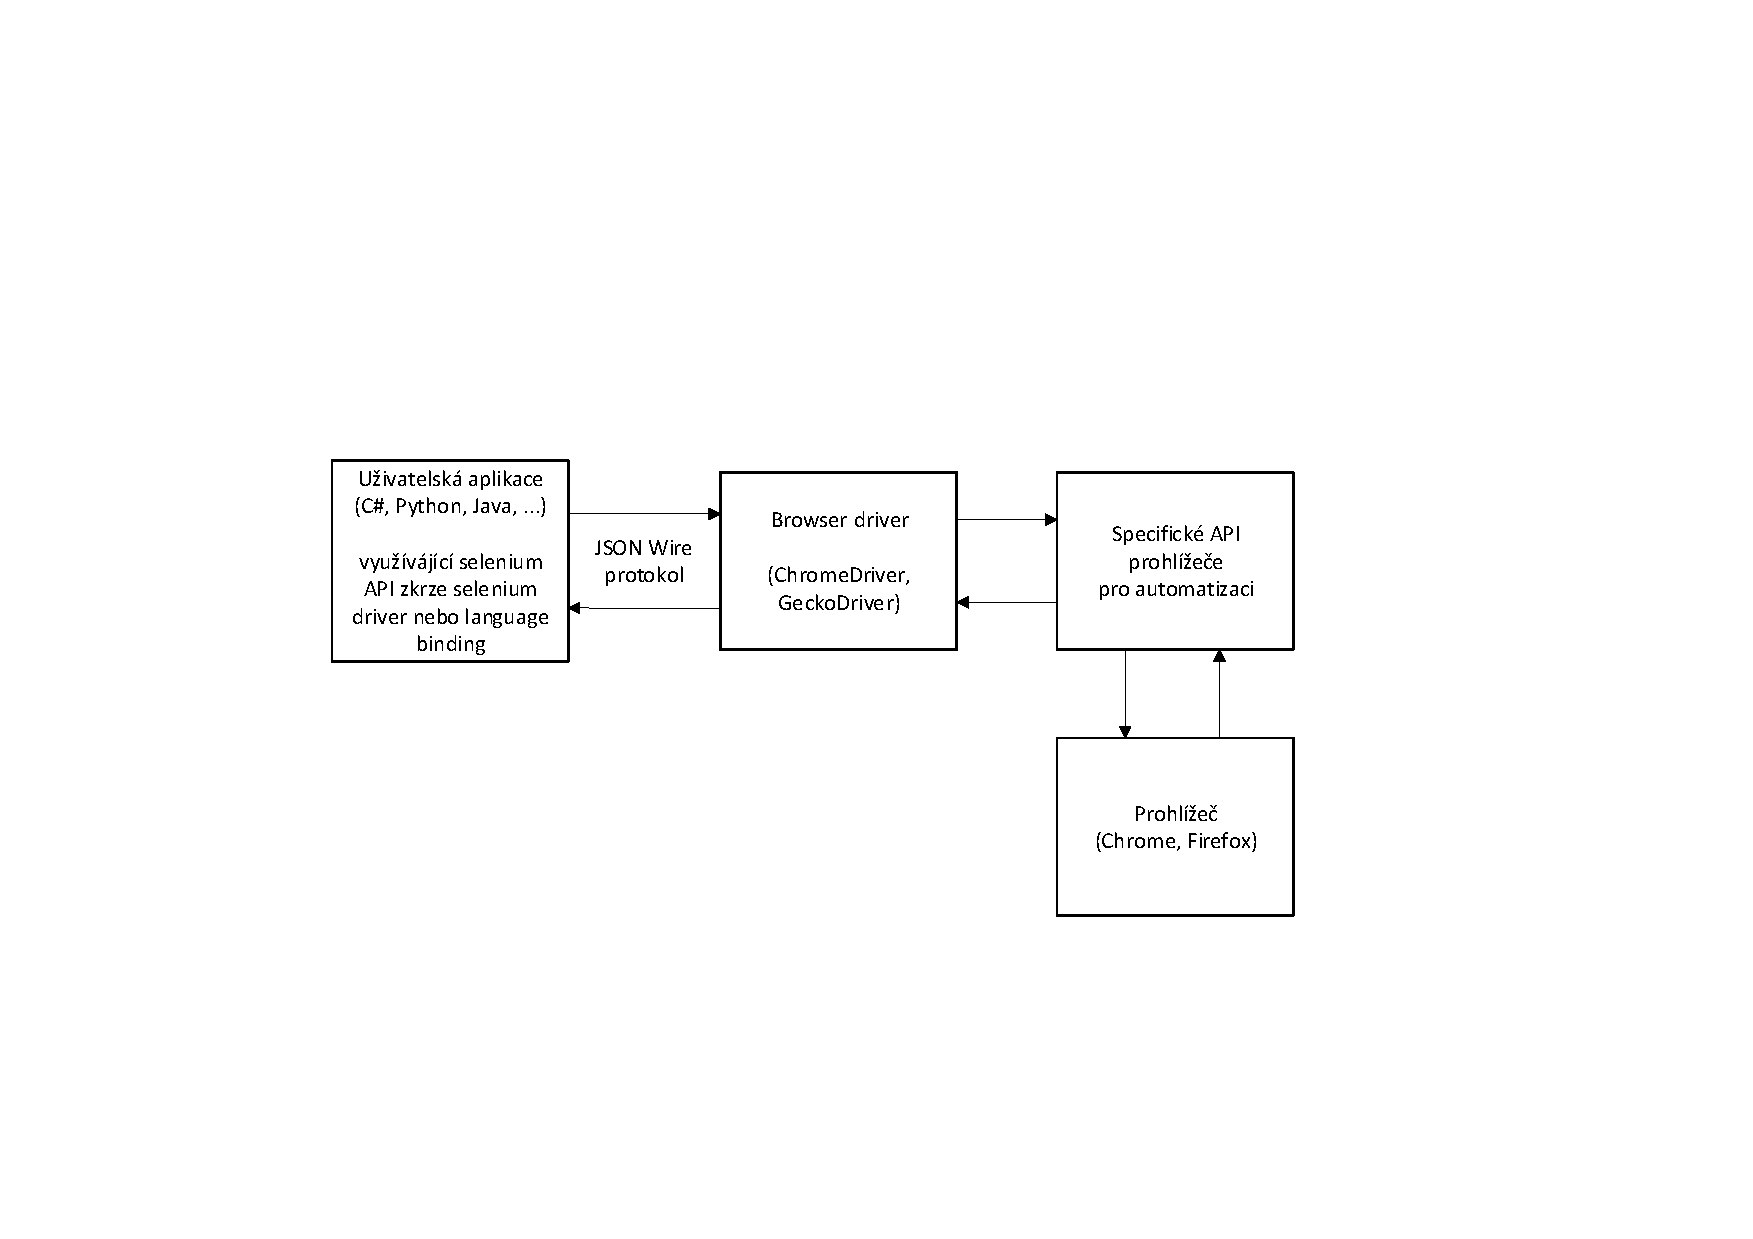
\includegraphics[width=1.0\textwidth]{seleniumCom.pdf}
		\caption{Komunikace Selenia s~prohlížečem}
	\end{figure}

	\noindent Přesuneme se ke~způsobu identifikace elementů na stránce. Dnes jsou v~selektorech verze 3 definovány rozmanitější selektory jako např. E\textasciitilde F, který vybere element F, kterému předchází element E~\cite{selectors3W3c}. Stále však není možné napsat selektor podle vlastnosti \texttt{textContent} elementu~\cite{selectors4W3c}. Může se to sice zdát zprvu nedůležité, avšak často se jedná o~dobrou identifikaci tlačítka, která je jednoznačná a~uživatelsky přívětivá.
	\begin{codefigure}[H]
		\renewcommand\baselinestretch{\codefigureSpacing}
		\begin{lstlisting}[style=MyHTML]
<button class="h51n1h-0" type="submit">Přihlásit se</button>
		\end{lstlisting}
		\caption{HTML kod tlačítka pro přihlášení}
		\label{codefig:loginButton}
	\end{codefigure}
	Předpokládejme, že tlačíko obsahuje jednoznačný text uvnitř tagů, pak bychom ho mohli identifikovat textem "Přihlásit se", namísto třídy, která může být generována na~session.
	
	\newpage
	Problém identifikace elementů byl v~Seleniu vyřešen pomocí rozšíření selektorů na tzv.~lokátory~\cite{seleniumDocs}.
	{
	\begin{table}[H]
		\centering
	\rowcolors{2}{alternatingRow}{white}  
%	\begin{longtable}{ l|l } 
	\begin{tabular}{ l|l }
	\rowcolor{tableHeadingBackground} \multicolumn{1}{l}{\textbf{Lokátor}} & \multicolumn{1}{l}{\textbf{Identifikuje element}} \\
	class name &  jehož třída obsahuje hledanou hodnotu.\\ 
	css selector & odpovídající hledanému selektoru. \\ 
	id & jehož atribut id odpovídá hledané hodnotě. \\
	name & jehož atribut name odpovídající hledané hodnotě. \\
	link text & jehož viditelný text odpovídající hledané hodnotě. \\
	partial link text & jehož viditelný text obsahuje hledanou hodnotu.  \\
	tag name & jehož název tagu odpovídá hledané hodnotě. \\
	xpath & odpovídající XPath dotazu. \\
%	\end{longtable}
	\end{tabular}
	\caption{Seznam lokátorů podporovaných Seleniem~\cite{seleniumDocs}}
	\label{tab:locatorsList}
	\end{table}
	}
	Tlačítko z~\cref{codefig:loginButton} bychom lokátory identifikovali jako \texttt{link text="Přihlásit se"}. Jediným však nezbytným lokátorem je XPath, s~jehož pouhým využitím je možné přepsat všechny ostatní lokátory.

	Mezi výhody Selenia patří podpora mnoha jazyků mezi kterými nechybí i~specifičtější jazyky jako např. Dart, Haskell a~R. Další výhodou je dobrá podpora napříč spektrem prohlížečů, obvykle včetně podpory všech OS, na kterých daný jazyk a~prohlížeč běží~\cite{seleniumDocs, seleniumEcosystem}.
	
	\begin{table}[H]
		\centering
		\rowcolors{2}{alternatingRow}{white}
		\begin{tabular}{ l|l|l } 
			\rowcolor{tableHeadingBackground}
			\multicolumn{1}{l}{\textbf{Prohlížeč}} & \multicolumn{1}{l}{\textbf{Podporované OS}} & \multicolumn{1}{l}{\textbf{Spravuje}}  \\
			Chromium/Chrome & Windows/macOS/Linux & Google \\ 
			Firefox & Windows/macOS/Linux & Mozilla \\ 
			Edge & Windows 10 & Microsoft \\
			Internet Explorer & Windows & Selenium Project \\
			Safari & macOS El Capitan a~novejší & Apple \\
			Opera & Windows/macOS/Linux & Opera
		\end{tabular}
		\caption{Podporované prohlížeče Seleniem~\cite{seleniumDocs}}
	\end{table}
	
	Hlavní nevýhodou, částečně vyplývající z~již zmíněných výhod, je omezená funkcionalita selenia API, podporující pouze to, co umí všechny prohlížeče, potažmo všechny browser drivery.
	\subsection{Puppeteer}
	\label{sub_sec:Puppeteer}
	Puppeteer je moderní Node.js knihovna, její počátky sahají pouze do roku 2017, kdy byla vydána první verze~\cite{puppeteerFirstRelease}. Puppeteer poskytuje API pro ovládání Chromu\footnote{Aktuálně již existují nightly verze Firefoxu s~FRP, jehož implementace je založená na~CDP. Platí, že FRP $\subset$ CDP. Je možné použít Puppeteer s~Firefoxem, ačkoliv se zatím jedná pouze o~experimentální podporu~\cite{firefoxRemoteProtocol, firefoxRemoteProtocol2}.}, narozdíl od Selenia se s~prohlížečem komunikuje pomocí Chrome DevTools Protocol (CDP). To hned nabízí jednu výhodu a~nevýhodu. Onou výhodou je podpora specifických a~proprietárních funkcí Chromu. Nevýhodou je právě však podpora pouze Chromu~\cite{puppeteerMainPage}.
	\begin{figure}[H]
		\centering	
		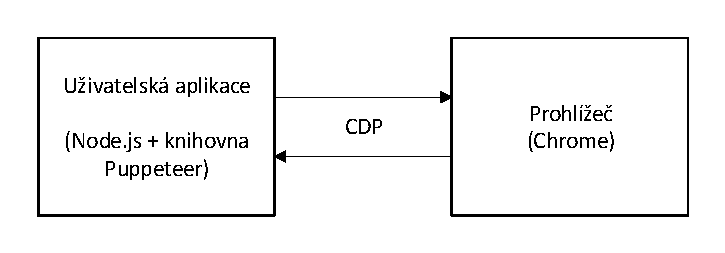
\includegraphics[width=1.0\textwidth]{puppeteerCom.pdf}
		\caption{Komunikace Puppeteeru s~Chromem}
	\end{figure}

	Puppeteer nelze zcela považovat za~konkurenci Selenia. Selenium se zaměřuje na~ automatizaci nezávisle na~prohlížeči. Jeho hodnotou je standardní API, které funguje ve všech hlavních prohlížečích. Puppeteer se narozdíl od toho zaměřuje na~Chrome. Hodnotou Puppeteeru je bohatší funkcionalita a~jednodušší API~\cite{puppeteerMainPage}. 
	
	Pro každou verzi Puppeteeru existuje právě jedna verze Chromu, se kterou je garantována funkčnost. 
	\begin{table}[H]
		\centering
		\rowcolors{2}{alternatingRow}{white}
		\begin{tabular}{ l|l } 
			\rowcolor{tableHeadingBackground}
			\multicolumn{1}{l}{\textbf{Verze Chromu}} & \multicolumn{1}{l}{\textbf{Verze Puppeteeru}} \\
			86.0.4240.0 & 5.3.0 \\ 
			85.0.4182.0 & 5.2.1 \\
			84.0.4147.0 & 5.1.0 \\
			83.0.4103.0 & 3.1.0
		\end{tabular}
		\caption{Několik odpovídajících verzí Chromu a~Puppeteeru~\cite{puppeteerApi}}
	\end{table}

	Z~tohoto důvodu existují dva balíčky. Prvním je balíček "puppeteer", který obsahuje kromě knihovny i~vestavěný Chrome odpovídající verze. Druhý balíček "puppeteer-core" obsahuje pouze knihovnu. "puppeteer-core", která se může hodit, pokud si chceme Chrome spravovat sami nebo se Puppeteerem chceme připojit na~vzdálený Chrome na~jiném počítači a~vestavěný by nám tak zabíral zbytečně místo~\cite{puppeteerMainPage}.
	
	Podíváme se na~několik ukázek porovnání Node.js kódu Puppeteeru a~Selenia. První ukázkou bude vytvoření screenshotu stránky \href{https://seznam.cz}{\nolinkurl{seznam.cz}}.
	 \begin{codefigure}[H]
		\begin{subfigure}[t]{\textwidth}
			\begin{lstlisting}[style=MyJavaScript]
const fs = require('fs')
const {Builder} = require('selenium-webdriver')
const chrome = require('selenium-webdriver/chrome');
	
(async () => {
	let driver = await new Builder().forBrowser('chrome')
	.setChromeOptions(new chrome.Options().headless())
	.build()

	await driver.get('http://seznam.cz')
	const imageData = await driver.takeScreenshot()
	fs.writeFileSync('C:\\scrnshot.png', imageData, 'base64')
	await driver.quit()
})() 
			\end{lstlisting}
			\caption{Node.js Selenium}
			\label{subfig:seleniumScreenshot}
		\end{subfigure}   
	\end{codefigure}
	\begin{codefigure}[H]\ContinuedFloat
		\begin{subfigure}[t]{\textwidth}
			\begin{lstlisting}[style=MyJavaScript]
const puppeteer = require('puppeteer');

(async () => {
	const browser = await puppeteer.launch()
	const page = (await browser.pages())[0]
	await page.goto('http://seznam.cz')
	await page.screenshot({path: 'C:\\scrnshot.png', fullPage: true})
	await browser.close()
})()
			\end{lstlisting}
			\caption{Puppeteer}
			\label{subfig:puppeteerScreenshot}
		\end{subfigure}
		\caption{Screenshot v~Node.js kódu}
	\end{codefigure}

	Kód \subref{subfig:seleniumScreenshot} i~\subref{subfig:puppeteerScreenshot} spustí Chrome v~headless režimu, načtou \href{https://seznam.cz}{\nolinkurl{seznam.cz}} a~uloží screenshot do souboru \path{C:\scrnshot.png}. Jediný rozdíl je ten, že kód \subref{subfig:puppeteerScreenshot} provede screenshot celé stránky, jak je nastaveno argumentem \texttt{fullPage: true}. Selenium API narozdíl od Puppeteeru neumožnuje provést screenshot celé stránky~\cite{seleniumNodeJsDocs} \label{text:seleniumFullPageScreenshot}.
	
	Druhá ukázka nechá vyhodnotit JavaScript uvnitř stránky prohlížeče a~výsledek vypíše na~výstup. Pro ušetření místa vynecháme v~této a~v~následující ukázkách této podsekce nedůležitý kód, zejména kód inicializující a~uklízející.
	\newpage
		 \begin{codefigure}[H]
		\begin{subfigure}[t]{\textwidth}
			\begin{lstlisting}[style=MyJavaScript]
const name = await driver.executeScript('return navigator.appName')
console.log(name)
			\end{lstlisting}
			\caption{Node.js Selenium}
		\end{subfigure}   
	\end{codefigure}
	\begin{codefigure}[H]\ContinuedFloat
		\begin{subfigure}[t]{\textwidth}
			\begin{lstlisting}[style=MyJavaScript]
const name = await page.evaluate(() => navigator.appName)
console.log(name)
			\end{lstlisting}
			\caption{Puppeteer}
		\end{subfigure}
		\caption{Node.js kód pro vyhodnocení JavaScriptu prohlížeče}
	\end{codefigure}

	V~tomto případě si můžeme všimnout, že se kód pro Selenium a~Puppeteer příliš neliší. Oba fragmenty kódu vypíší textový řetězec "Netscape", protože hodnota \texttt{navigator.appName} je takto definována~\cite{navigator.appName}.
	
	Existují však i~situace, kdy je jednodušší napsat kód pro Selenium, než pro Puppeteer, viz následující ukázka.
\begin{codefigure}[H]
	\begin{subfigure}[t]{\textwidth}
		\begin{lstlisting}[style=MyJavaScript]
await driver.findElement(By.linkText('About')).then(e => e.click())
await driver.findElement(By.name('options')).then(e => e.click())
		\end{lstlisting}
		\caption{Node.js Selenium}
	\end{subfigure}   
\end{codefigure}
\begin{codefigure}[H]\ContinuedFloat
	\begin{subfigure}[t]{\textwidth}
		\begin{lstlisting}[style=MyJavaScript]
await page.$x("//*[text() = 'Grading']").then(es => es[0].click())
await page.$x("//*[@name = 'options']").then(es => es[0].click())
		\end{lstlisting}
		\caption{Puppeteer}
	\end{subfigure}
	\caption{Node.js kód pro kliknutí na~element}
\end{codefigure}

První řádek i~druhý řádek vždy obsahují kód, který nalezne a~stiskne element. V~případě prvního řádku se stiskne element s~textovým popiskem "About". Na~druhém řádku se stiskne element obsahující atribut \texttt{name} s~hodnotou "options". Puppeteer narozdíl od Selenia nemá lokátory, elementy můžeme hledat pouze pomocí selektoru a~naštěstí i~XPathu\label{text:puppeteerLocatorSupport}~\cite{puppeteerApi}.

	\newpage
	\subsection{Playwright}
	\label{sub_sec:Playwright}
	Playwright je ryze moderní záležitostí vyvíjenou společností Microsoft vydanou teprve v~druhém měsici roku 2020~\cite{playwrightFirstRelease}. Původně jde pouze o~fork knihovny Puppeteer. Playwright však dává důraz na jiné aspekty funkcionality~\cite{playwrightGithub}.
	
	\paragraph{Rozdíly proti Puppeteeru}
	Playwright nabízí jednotné API pro automatizaci Chromu, Firefoxu a~prohlížečů postavených na jádře WebKit~\cite{playwrightMainPage}. Aktuálně však je bez úprav podporovaný pouze Chrome. Ostatní prohlížeče musí být speciálně upraveny pomocí patchů, aby bylo možné jejich použití s~Playwrightem. Pro Playwright by bylo ideální sloučení těchto patchů se zdrojovými kódy prohlížečů, v~budoucnu by k~tomu mohlo dojít. Některé patche již byly přijaty.~\cite{playwrightBrowserPatches}.
	
	Další změnou je automatické čekání na elementy, před provedením akce s~nimi~\cite{playwrightMainPage}. První ukázku kódu pro Playwright uvedeme korektně včetně inicializace a~uklízení. Všechny další ukázky této podsekce budou obsahovat pouze nezbytný kód.
	\begin{codefigure}[H]
		\begin{subfigure}[t]{\textwidth}
			\begin{lstlisting}[style=MyJavaScript]
const { chromium } = require('playwright');

(async () => {
	const browser = await chromium.launch({headless: false})
	const page = await browser.newPage()
	await page.goto('https://webik.ms.mff.cuni.cz')
	await page.click('#navlink_tab_grading') (*@\label{line:playwrightClickSelector}@*) 
	await browser.close()
})()
			\end{lstlisting}
			\caption{Korektní kód pro Playwright}
			\label{subfig:playwrightCorrectClick}
		\end{subfigure}   
	\end{codefigure}
	\begin{codefigure}[H]\ContinuedFloat
		\begin{subfigure}[t]{\textwidth}
			\begin{lstlisting}[style=MyJavaScript]
await page.goto('https://webik.ms.mff.cuni.cz')
await page.click('#navlink_tab_grading')
			\end{lstlisting}
		\begin{tikzpicture}[remember picture,overlay]
			\draw[color=black, line width=0.25mm](0,0) -- (14.5,2);
			\draw[color=black, line width=0.25mm](0,2) -- (14.5, 0);
		\end{tikzpicture}
		\caption{Nekorentní kód pro Puppeteer}
		\label{subfig:puppeteerIncorrectClick}
		\end{subfigure}
	\end{codefigure}
	\begin{codefigure}[H]\ContinuedFloat
	\begin{subfigure}[t]{\textwidth}
		\begin{lstlisting}[style=MyJavaScript]
await page.goto('https://webik.ms.mff.cuni.cz')(*@\label{line:puppeteerNavigation}@*)
await page.waitForSelector('#navlink_tab_grading')(*@\label{line:puppeteerWaitForSelector}@*) 
await page.click('#navlink_tab_grading')
		\end{lstlisting}
		\caption{Korektní kód pro Puppeteer}
		\label{subfig:puppeteerCorrectClick}
	\end{subfigure}
	\captionsetup{justification=centering}
	\caption{Porovnání kódu Playwrightu a~Puppeteeru pro stisk elementu po~navigaci}
	\end{codefigure}
	Kód \subref{subfig:playwrightCorrectClick} na~\lineref{line:playwrightClickSelector}{řádku} před klikem počká až element bude dostupný na stránce~\cite{playwrightApi}. Naproti tomu \subref{subfig:puppeteerIncorrectClick} na element nečeká a~pokud se nevyskytuje na stránce, tak vyhodí okamžitě výjimku~\cite{puppeteerApi}. Vzhledem k~povaze dnešního webu je žádoucí si zkontrolovat a~případně počkat na dynamické načtení elementů pomocí JavaScriptu. V~Puppeteeru to můžeme zajistit viz \lineref{line:puppeteerWaitForSelector}{řádek} \subref{subfig:puppeteerCorrectClick}~\cite{puppeteerApi}. Povšimněme si, že speciálně kód na~\lineref{line:puppeteerNavigation}{řádku} \subref{subfig:puppeteerCorrectClick} nevyžaduje obdobné volání, které by počkalo na dokončení navigace. Puppeteer totiž automaticky čeká na volání "load" události~\cite{loadEvent} uvnitř stránky~\cite{puppeteerApi}.
	
	Chování Playwrightu a~Puppeteeru při navigaci a~libovolné akci s~elementem nám shrnuje následující tabulka.
	\begin{table}[H]
		\centering
%		\rowcolors{2}{alternatingRow}{white}
		\begin{tabular}{l|m{0.23\linewidth}|m{0.18\linewidth}| p{0.25\linewidth} } 
			\rowcolor{tableHeadingBackground}
			\multicolumn{1}{l}{\textbf{Knihovna}} & \multicolumn{1}{l}{\textbf{Akce s~elementem}} & \multicolumn{1}{l}{\textbf{Navigace}} &
			\multicolumn{1}{l}{\textbf{Vynutit čekání}}  \\
			Playwright & Čeká 30s, pokud se neobjeví, tak výjimka. & \multirow{2}{3cm}{Čeká max 30s na~zavolání "load" události, jinak výjimka.} & \strike{l}{} \\ \cline{2-2}
			Puppeteer & Pokud neexistuje, tak výjimka. & & Voláním odpovídající "waitFor..." metody.
		\end{tabular}
		\caption{Porovnání čekání Playwrightu a~Puppeteeru~\cite{playwrightApi, puppeteerApi}}
	\end{table}

	Jak již bylo zmíněno v~\partialref{text:puppeteerLocatorSupport}{sub_sec:Puppeteer} v~Puppeteeru je možné identifikovat element pouze pomocí selektoru a~XPath, což sice nesnižuje sílu pro identifikaci, ale nutí nás psát si vlastní nestandardní rozšíření, nebo stále dokola psát XPath dotazy. Mezi další funkce Playwrightu patří, obdobně jako lokátory v~Seleniu, sofistikovanější prostředky pro identifikaci elementů~\cite{playwrightApi}. 
	\begin{codefigure}[H]
		\renewcommand\baselinestretch{\codefigureSpacing}
		\begin{lstlisting}[style=MyJavaScript]
await page.click('text="banán"')(*@\label{line:bananaClick}@*)
await page.type('[data-purpose="amount"]', '42')(*@\label{line:amountType}@*)
await page.check((*@\label{line:check1}@*)
	'css=form[method = "POST"] >> css=input[type = "checkbox"]')(*@\label{line:check2}@*)
		\end{lstlisting}
		\caption{Akce se specificky identifikovanými elementy}
	\end{codefigure}
	Na \ref{line:bananaClick}. řádku se provede stisknutí elementu s~textovým popiskem "banán". Další řádek "napíše" hodnotu 42 do~elementu s~atributem \foreignlanguage{english}{\texttt{data-purpose = "amount"}}. Poslední nejdelší řádek obsahuje speciální binární, zleva asociativní operátor \texttt{>>}. Pravý operand se vyhodnotí vzhledem k~elementům splňující levý operand~\cite{playwrightApi}. V~tomto případě se hledá checkbox pro zaškrtnutí pouze uvnitř formuláře odesílaného POST metodou. Ekvivalentně bychom mohli použít XPath:
	\begin{codefigure}[H]
		\renewcommand\baselinestretch{\codefigureSpacing}
		\begin{lstlisting}[style=MyXPath]
//form[@method="POST"]//input[@type="checkbox"]
		\end{lstlisting}
	\caption{XPath ekvivalentní identikátoru elementu na~\lineref{line:check2}{řádku}}
	\end{codefigure}
	
	Unikátní a~zajímavá funkce, kterou disponuje pouze Playwright je API pro stahování souborů. Použití je následující~\cite{playwrightApi}: 
	\begin{enumerate}
		\item Stránka, potažmo kontext\footnote{Prostředí jedné i~více stránek prohlížeče. Obvykle se sdíleným nastavením, např. neukládat historii. Při používání Chromu můžeme vytvořit nový kontext otevřením prvního okna anonymního režimu, zkratka CTRL+Shift+N. Pokud takto otevřeme další okna, nevytvoří se nový anonymní kontext, pouze se nová stránka přidá do již existujícího anonymního kontextu.} prohlížeče, ve kterém stránka běží, musí mít nastavený parametr \texttt{acceptDownloads: true}.
		\item Při provedení akce, která způsobí stažení souboru musíme počkat na~událost "download" a~zachytit zachytit objekt \texttt{Download}. 
		\item Nyní již libovolně můžeme využít API objektu \texttt{Download} a~stažený soubor např. uložit do libovolného adresáře. 
	\end{enumerate}

	Uvedeme jednoduchý příklad, který stáhne instalátor Firefoxu a~uloží ho na~disk C s~původním názvem.
	\begin{codefigure}[H]
	\renewcommand\baselinestretch{\codefigureSpacing}
	\begin{lstlisting}[style=MyJavaScript]
const page = await browser.newPage({acceptDownloads: true})
await page.goto('https://www.mozilla.org/cs/firefox')

const [download] = await Promise.all([
	page.waitForEvent('download'),
	page.click('[data-download-os="Desktop"]')
])

await download.saveAs('C:\\' + download.suggestedFilename())
	\end{lstlisting}
	\caption{Stažení instalátoru Firefoxu}
\end{codefigure}
	\newpage
	\subsection{PhantomJS}
	Podíváme se ještě krátce na~značně odlišnou záležitost, která již není od března roku 2018 aktivně vyvíjena~\cite{phantomJsArchiving}. Zatím jsme v~\refAddedText{section:introToBrowserAut}{kapitole }{} rozebírali jednotlivé technologie pro automatizaci existujících standardních prohlížečů. PhantomJS je však kompletní prohlížeč navržený tak, aby byl skriptovatelný. Jednou z~jeho přednosti ve své době patřilo headless spouštění~\cite{phantomJsMainPage}, které se ve~Chromu objevilo až s~verzí 59 pro macOS a~Linux, podpora Windowsu pak byla přidána ve~verzi 60~\cite{headlessChromeGettingStarted}. Firefox jednotně podporoval headless režim na macOS/Linuxu/Windowsu od verze 56~\cite{headlessFirefox}.
	
	\begin{table}[H]
		\centering
		\rowcolors{2}{alternatingRow}{white}
		\begin{tabular}{ l|l } 
			\rowcolor{tableHeadingBackground}
			\multicolumn{1}{l}{\textbf{Prohlížeče}} & \multicolumn{1}{l}{\textbf{Datum vydání}} \\
			Chrome 59 & červen 2017 \\ 
			Chrome 60 & červenec 2017 \\
			Firefox 56 & listopad 2017 \\
			PhantomJS 1.0.0 & leden 2011
		\end{tabular}
		\captionsetup{justification=centering}
		\caption{Porovnání datumu vydání prvních verzí prohlížečů podporujících \mbox{head\-less} režim~\cite{googleChromeReleases, firefoxReleaseCalendar, phantomJsFirstRelease}}
	\end{table}
	Z~tabulky je patrné, že PhantomJS si držel konkurenční výhodu dlouhých 6~let. Po její ztrátě již netrvalo dlouho a~projekt byl archivován.
	
	Na závěr si ukážeme fragment kódu využívající Node.js binding pro Phan\-tomJS. Provedeme screenshot celé stránky \href{https://www.mff.cuni.cz}{\nolinkurl{mff.cuni.cz}} a~uložíme ho jako \mbox{\path{C:\scrnshot.pdf}}.
	\begin{codefigure}[H]
		\renewcommand\baselinestretch{\codefigureSpacing}
		\begin{lstlisting}[style=MyJavaScript]
const phantom = require('phantom');

(async () => {
	const browser = await phantom.create()
	const page = await browser.createPage()
	await page.open('https://mff.cuni.cz')
	await page.render('C:\\scrnshot.pdf')
	await browser.exit()
})()
	\end{lstlisting}
		\caption{Uložení screenshotu celé stránky do PDF s~využítím PhantomJS}
	\end{codefigure}
	
	Obdobně jednoduchým způsobem je možné vytvořit screenshot s~uložením do PDF i~s~použitím Puppeteeru nebo Playwrightu. V~případě použití Selenia je nutné se omezit pouze výstup v~obrázkovém formátu\cite{seleniumDocs} a~na~screenshot viewportu, jak již bylo zmíněno v~\fullref{text:seleniumFullPageScreenshot}{sub_sec:Puppeteer}.
	\section{Nahrávání a~přehrávání akcí}
	V~této kapitole se podíváme na řešení sloužící k~zaznamenávání uživatelských akcí v~prohlížeči s~možností následného opětovného vykonání, dále pouze uváděno jako řešení pro nahrávání a~přehrávání akcí nebo pouze řešení.
	
	Nejprve se podíváme na vybraná existující konkurenční řešení. Podsekce \fullNameref{sub_sec:existingSolutions} slouží k~představení běžných zástupců řešení k~automatizaci prohlížeče, zde jsou uvedeni zástupci s~open-source i~proprietárními licencemi. Hlavním významem této podsekce je ukázání existence/neexistence funkcí představených řešení. Tyto řešení jsou pak porovnány s~vlastním řešení v~\ref{sub_sec:functionalityComparison}. 
	
	Později v~\ref{sub_sec:PuppeteerUsageForAutomation} se zaměříme výhradně na Puppeteer, zde provdeneme detailní rozbor možností Puppeteeru pro nahrávání a~přehrávání akcí včetně ukázek kódu demonstrující využití.
	\subsection{Konkurenční řešení}
	\label{sub_sec:existingSolutions}
	V~této části se výhradně zaměříme na konkurenční řešení. Podíváme se na jejich funkcionalitu, popíšeme výhody a~nevýhody. %výhody, nevýhody a~porovnáme je mezi sebou.
	
	Přikládáme ještě tabulku primárně určenou pro rychlou orientaci v~této sekci a~jednoduché porovnání.
{
	\rowcolors{2}{alternatingRow}{white}  
	\begin{longtable}{ l|l|l|c|c } 
		\rowcolor{tableHeadingBackground} \multicolumn{1}{l}{\textbf{Název}} & \multicolumn{1}{l}{\textbf{Využívá}} & \multicolumn{1}{l}{\textbf{Licence}} & \multicolumn{1}{l}{\textbf{Nahrávání}} & \multicolumn{1}{l}{\textbf{Přehrávání}} \\
		Selenium IDE & Selenium & Apache License 2.0 & \cmark & \cmark \\
		Katalon Recorder & Selenium & Apache License 2.0 & \cmark & \cmark \\
		Ranorex Recorder & \multicolumn{2}{c}{Proprietární} & \cmark & \cmark \\
		Headless Recorder & Puppeteer & Apache License 2.0 & \cmark & \xmark \\
		\caption{Orientační porovnání existujících řešení}
	\end{longtable}
}
	\subsubsection{Selenium IDE}
	Selenium IDE je nástroj postavený nad Seleniem viz \ref{sec:selenium} fungující jako rozšíření Chromu a~Firefoxu. Původně ho navrhl Shinya Kasatani, který umožnil v~roce 2006 jeho vstup mezi oficiální nástroje Selenia~\cite{seleniumHistory, seleniumIdeGithub}.
	
	V~roce 2017, kdy byla aktuální v2 Selenia IDE, se projekt dostal do problémů, kód v~té době fungoval pouze s~Firefoxem a~byl závislý na specifickém API Firefoxu pro add-ony~\cite{seleniumWhyUse}. Těmto add-onům se dnes říká "legacy extensions", ve Firefoxu byla jejich podpora úplně odstraněna s~verzí 57~\cite{firefoxLegacyExtensions}, která vyšla ve stejném roce~\cite{firefoxReleaseCalendar}. Projekt se však díky práci vývojářů podařilo udržet naživu.
	
	Aktuálně existují dvě vyvíjené větve, první je v3, ve které se stále ještě přepisují některé části kódu starého Selenia IDE v2. Cílem v3 je podpora moderních aktuálních verzí prohlížečů Chrome a~Firefox včetně všech funkcí původního Selenia IDE v2~\cite{seleniumIdeGithub}.
	
	Druhou větví je master, ve které se pracuje na přechodu z~rozšíření Chromu a~Firefoxu na Electron. V~současné době však zatím nebyla vydána žádná verze fungující s~Electronem. Zájemci o~vyzkoušení mají možnost si zdrojový kód zkompilovat sami~\cite{seleniumIdeGithub}.
	
	Léta vývoje se projevují na funkcionalitě, pojďme se na některé zajímavé funkce Selenia IDE v3.17.0, současně nejnovější verze dostupné~\cite{seleniumIdeReleses}, podívat.
	
	\paragraph{Výběr z~lokátorů}
	Pro každý element se nalezne sada lokátorů, uživatel si může vybrat ten nejvhodnější.
	\begin{figure}[H]
		\centering
		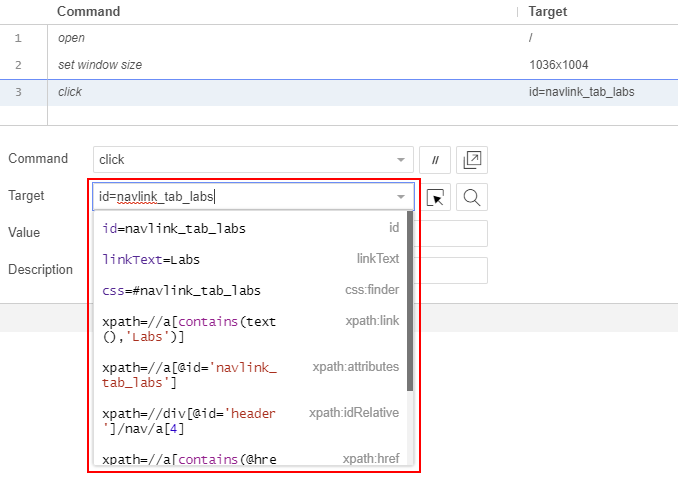
\includegraphics[width=1.0\textwidth]{locatorsSelect.png}
		\caption{Výběr z~lokátorů identifikujících element}
	\end{figure}
	\newpage
	\paragraph{Změna elementu klikem myši}
	Pro změnu elementu na němž se má akce provést, aniž bychom museli ručně přepisovat lokátor, existuje tlačítko umožňující znovu zachytit element.
	\nopagebreak
	\begin{figure}[H]
		\centering
		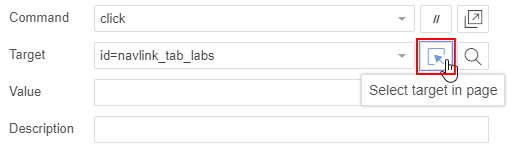
\includegraphics[width=0.92\textwidth]{changeElement.png}
	\end{figure}
	\vspace{-0.7cm}
	\begin{figure}[H]
		\centering
		\begin{minipage}{0.5\textwidth}
			\textdownarrow	
		\end{minipage}
	\end{figure}
	\vspace{-0.7cm}
	\begin{figure}[H]
		\centering
		\begin{subfigure}{0.47\textwidth}
			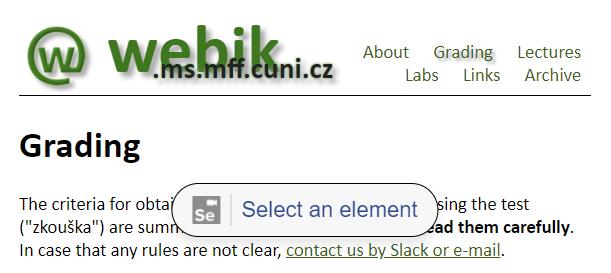
\includegraphics[width=1\textwidth]{changeElement2.png}
		\end{subfigure}
		\textrightarrow
		\begin{subfigure}{0.47\textwidth}
			
\includegraphics[width=1\textwidth]{changeElement3.png}
		\end{subfigure}
		\caption{Změna elementu bez ručního přepisování lokátoru}
	\end{figure}
	\paragraph{Zobrazení nalezeného elementu}
	Pokud chceme zpětně zjistit jaký element je lokátorem identifikován, stačí kliknout na~tlačítko s~obrázkem lupy, identifikovaný element se uvnitř stránky zvýrazní.
	\begin{figure}[H]
		\centering
		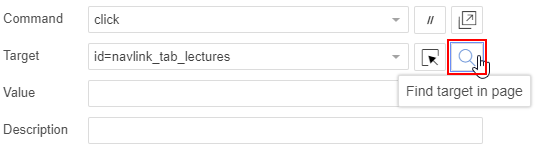
\includegraphics[width=0.97\textwidth]{findElement.png}
	\end{figure}
	\vspace{-0.7cm}
	\begin{figure}[H]
		\centering
		\textdownarrow
	\end{figure}
	\vspace{-0.7cm}
	\begin{figure}[H]
		\centering
		
\includegraphics[width=0.8\textwidth]{findElement2.png}
		\caption{Zpětné zobrazení identifikovaného elementu}
	\end{figure}
	\paragraph{Mouseover}
	Mnoho elementů na stránce je často skryto, dokud nepřejedeme myší přes nabídkový element, jehož JavaScript způsobí odkrytí elementů. 
	\nopagebreak
	\begin{figure}[H]
		\centering
		\begin{subfigure}{0.49\textwidth}
			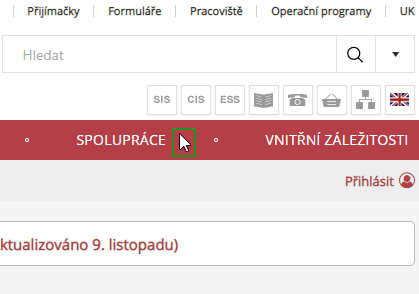
\includegraphics[width=0.97\textwidth]{mouseover.png}
			\caption{Kurzor mimo nabídku}
		\end{subfigure} \hfill
		\begin{subfigure}{0.49\textwidth}
			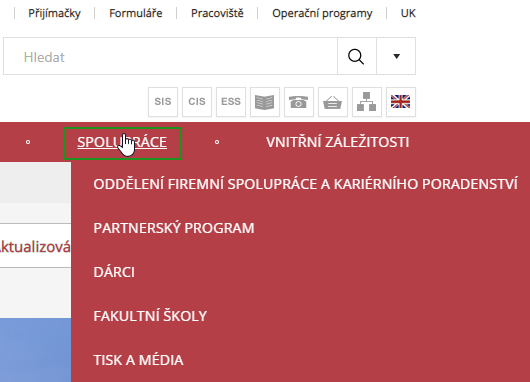
\includegraphics[width=0.95\textwidth, center]{mouseover2.png}
			\caption{Kurzor přejíždějící přes nabídku}
		\end{subfigure}
		\caption{Stránky MFF UK s~nabídkovým elementem}
	\end{figure}
	Není vhodné zaznamenávat veškeré pohyby kurzoru přes elementy. Většina z~nich nezpůsobuje žádný efekt na stránce, pouze nám zahlcují nahrávač přebytečnými událostmi a~snižují přehlednost. Jak však nahrát nezbytná přejetí kurzoru přes element? Ukážeme si jak je tento problém vyřešen v~Seleniu IDE.
	
	Implicitně se nezaznamenávájí žádné "mouseover" události. Zaznamenání si však můžeme explicitně vyžádat.
	\begin{figure}[H]
		\centering
		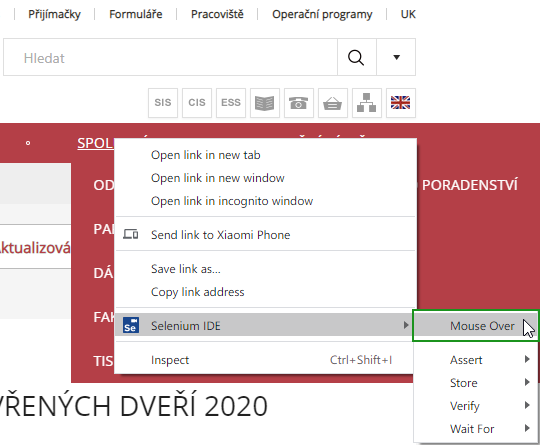
\includegraphics[width=0.8\textwidth]{mouseover3.png}
		\caption{Explicitní zaznamenání "mouseover" akce}
	\end{figure}
	\paragraph{Debugger}
	Selenium IDE se tak nejmenuje náhodně. Jeho součástí je plnohodnotný debugger, včetně breakpointů, krokování, tak jak ho můžeme znát z~IDE. 
	\nopagebreak
	\begin{figure}[H]
		\centering
		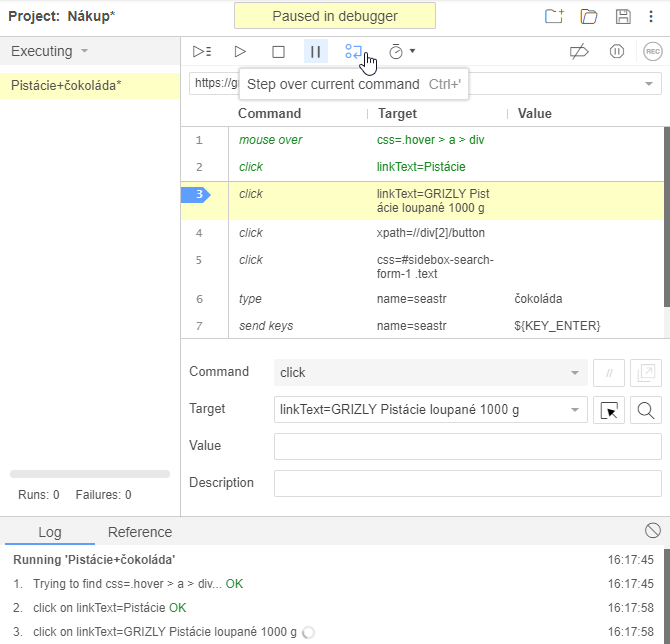
\includegraphics[width=1.0\textwidth]{seleniumIdeDebugger.png}
		\caption{Přehrávání s~breakpointem na 3. akci}
	\end{figure}
	
	\noindent Obraťme pohled na nevýhody, mezi větší nevýhodu aktuálního Selenia IDE v3, než by se na první pohled mohlo zdát, patří jeho návrh závislý na API prohlížečů pro extensiony. Dnes v3 je extension pro Chrome i~Firefox, oproti v2, která byla závislá na~specifickém API Firefoxu, fungující pouze s~Firefoxem. Nicméně úplné osvobození od API prohlížečů přijde až s~vydáním verze postavené na Electronu.
	
	Kritickou záležitostí aktuálního Selenia IDE v3 je, že může komunikovat pouze s~instancí prohlížeče, která ho spustila, tzn. že nemůže komunikovat s~prohlížečem bez nainstalovaného extensionu, připadně s~prohlížečem běžícím na~vzdáleném počítači.
	\subsubsection{Katalon Recorder}
	Katalon Recorder je produkt společnosti Katalon LLC. Původně jde o~fork Selenia IDE, již od vydání první veřejné verze v~roce 2016 Katalon Recorder fungoval s~Chromem a~Firefoxem~\cite{katalonRecorderMainPage, katalonRecorderWikipedia}. Zejména v~roce 2017, kdy Selenium IDE fungovalo pouze s~Firefoxem a~využívalo jeho historické, odstraněné API, byl Katalon Recorder velmi silný významný konkurent. Vzhledem k~tomu, že se dnes Selenium IDE ze svých problémů dostalo, se jedná o~dvě velmi podobná a~srovnatelná řešení.
	\begin{figure}[H]
		\begin{subfigure}{0.49\textwidth}
			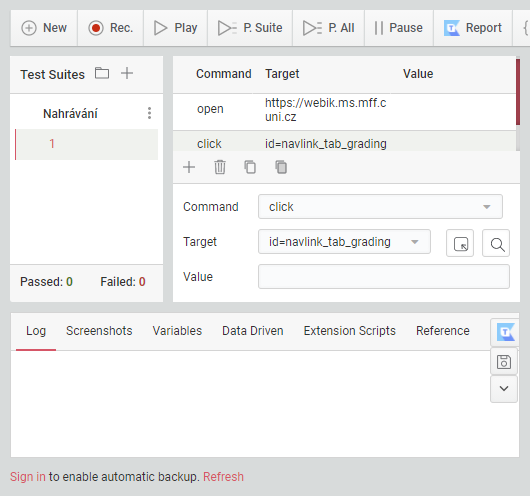
\includegraphics[width=0.97\textwidth]{katalonRecorderUi.png}
			\caption{Katalon Recorder}
		\end{subfigure} \hfill
		\begin{subfigure}{0.49\textwidth}
			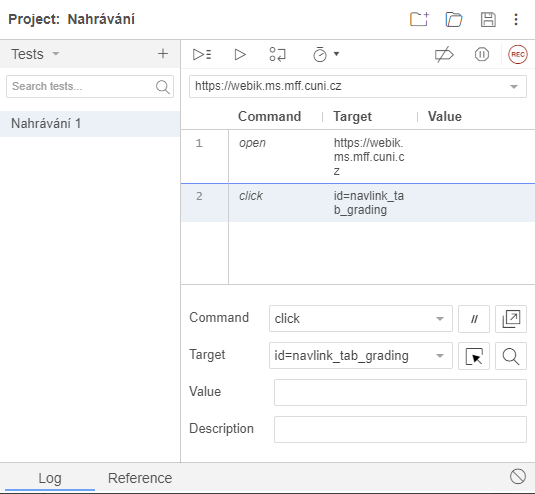
\includegraphics[width=0.97\textwidth, center]{seleniumIdeUi.png}
			\caption{Selenium IDE}
		\end{subfigure}
		\caption{Porovnání GUI Katalon Recorderu a~Selenia IDE}
	\end{figure}
	
	Hlavním důvodem pro upřednostnění Katalon Recorderu při výběru mezi různými existujícími řešeními je jeho placená varianta Katalon Studio Enterprise, ve které je zahrnuta podpora produktu, ale i~rozšířené funkce. Jednou takovou funkcí je "self-healing execution", tj.~využití nalezených náhradních lokátorů, pokud vybraný selže~\cite{katalonPricing}. Existují ale i~další méně patrné funkce Katalon Recorderu zahrnuté i~ve volně dostupné verzi, které Selenium IDE nemá.
	\begin{figure}[H]
		\begin{subfigure}[t]{0.6\textwidth}
			%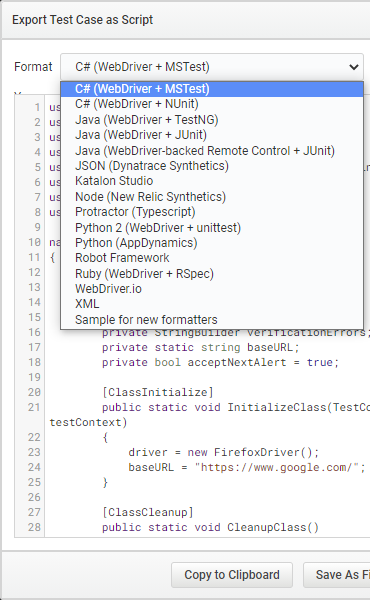
\includegraphics[scale=0.4]{katalonRecorderExport.png}
			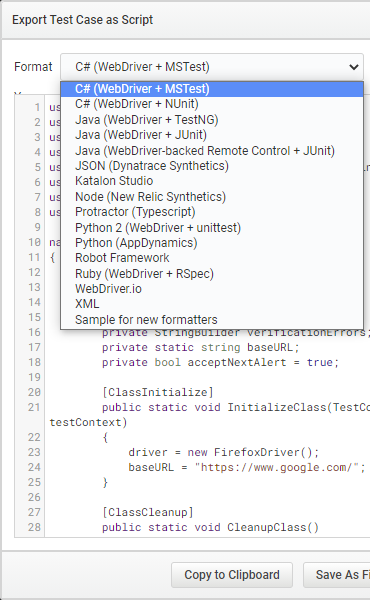
\includegraphics[width=1.0\textwidth]{katalonRecorderExport.png}
			\caption{Katalon Recorder}
		\end{subfigure} \hfill
		\begin{subfigure}[t]{0.37\textwidth}
			%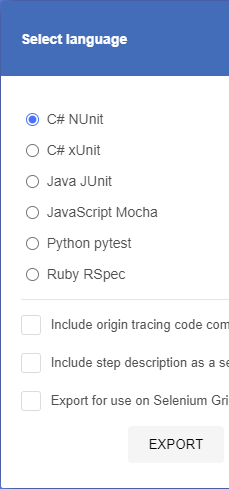
\includegraphics[scale=0.656, center]{seleniumIdeExport.png}
			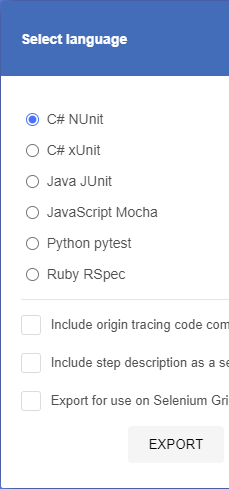
\includegraphics[width=1.0\textwidth, center]{seleniumIdeExport.png}
			\caption{Selenium IDE}
		\end{subfigure}
		\caption{Porovnání podporovaných jazyků pro export}
		\label{fig:katalonExportComparison}
	\end{figure}
	Jak \cref{fig:katalonExportComparison} výše ukazuje, Katalon Recorder dokáže exportovat nahrané akce do většího počtu různých technologií, narozdíl od Selenia IDE.
	
	Na druhou stranu v~Katalon Recorderu jsou dostupné pouze tři lokátory a~těmi jsou id, name a~xpath~\cite{katalonRecorderVsStudio} (seznam lokátorů viz \crefAddedText{tab:locatorsList}{}{ na~straně \pageref{tab:locatorsList}}). Ostatní jsou zpřístupněny až v~Katalon Studiu Enterprise a~Katalon Studiu~\cite{katalonRecorderVsStudio}, což je bezplatná varianta Katalon Studia Enterprise postrádající mimo jiné podporu. Ani tuto variantu není možné stáhnout bez vytvoření Katalon účtu vyžadujícího jméno, email, heslo a~zodpovězení dvou otázek~\cite{katalonPricing}.
	\newpage
    \subsubsection{Ranorex Recorder}
    Velmi krátce zmíníme jedno proprietární komerční řešení, tím je Ranorex Recorder, který je součástí balíčku Ranorex Studio sloužící pro automatizaci GUI a~prohlížečů. Původně byl tento produkt vytvořen v~Rakousku v~roce 2007 jakožto volně dostupná aplikace. Následná popularita aplikace vedla k~vývoji komerční verze s~podporou, která byla v~roce 2017 odkoupena americkou společností IDERA, Inc~\cite{ranorexAbout}.
    
    Pomineme GUI a~zaměříme se pouze na automatizaci prohlížečů, její funkčnost je zajištěna na~bází komunikace externí aplikace Ranorex Recorderu a~prohlížeče resp. jeho rozšíření Ranorex Automation. Mezi prohlížeče, pro které existuje rozšíření Ranorex Automation a~jsou proto podporovány, patří Internet Explorer, Firefox a~Chrome.
	\subsubsection{Headless Recorder (dříve Puppeteer Recorder)}
	Jediným řešením postaveným na Puppeteeru, o~kterém se zmíníme je Headless Recorder od společnosti Checkly, Inc. Řešení je postavené nad Puppeteerem, a~proto je kompatibilní pouze s~Chromem. Celá implementace je provedena jako rozšíření prohlížeče, nejedná se o~úplné řešení umožňující nahrávání a~přehrávání akcí. Podporované je pouze zaznamenávání několika málo akcí a~vygenerování Puppeteer kódu~\cite{checkly}.
	\newpage
	\begin{figure}[H]
		\centering
		\begin{subfigure}{0.47\textwidth}
			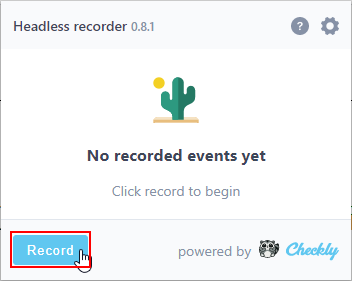
\includegraphics[width=1\textwidth]{headlessRecorder1.png}
		\end{subfigure}
		\textrightarrow
		\begin{subfigure}{0.47\textwidth}
			\begin{adjustwidth}{0.2cm}{0cm}
				Zaznamenáme akce, jejichž kód chceme vygenerovat.
			\end{adjustwidth}
		\end{subfigure}
	\end{figure}
	\hfill
	\begin{minipage}{0.5\textwidth}
		\centering
		\vspace{-4.0cm}
		\textdownarrow	
	\end{minipage}
	\begin{figure}[H]\ContinuedFloat
		\centering
		\begin{subfigure}{0.47\textwidth}
			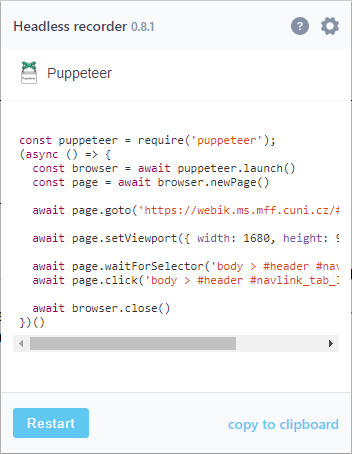
\includegraphics[width=1\textwidth]{headlessRecorder4.png}
		\end{subfigure}
		\textleftarrow
		\begin{subfigure}{0.47\textwidth}
			\vspace{-3.0cm}
			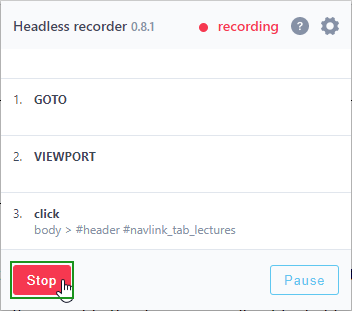
\includegraphics[width=0.97\textwidth, right]{headlessRecorder3.png}
		\end{subfigure}
		\caption{Použití Headless Recorderu}
	\end{figure}
	
	\newpage
	\paragraph{Funkcionalita}
	Mezi zaznamenávané akce patří základní události jako stisk klávesy a~myši. Podpora "mouseover" události v~jakékoliv podobě chybí stejně jako podpora lokátorů či případných jiných rozšířeních selektorů.
	
	V~nastavení je k~dispozici, jak ukazuje následující obrázek, pouze několik položek, jejichž význam je zřejmý.
    \begin{figure}[H]
		\centering
		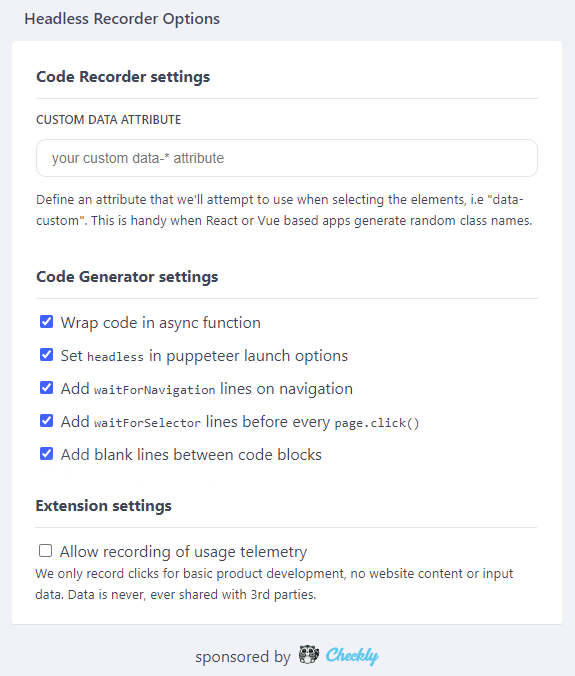
\includegraphics[width=1.0\textwidth]{headlessRecorderSettings.png}
		\caption{Nastavení Headless Recorderu}
	\end{figure}
	
	\noindent Právě jedním ze zásadních důvodů pro vytvoření této práce byly chybějící pokročilé funkce jako např. nemožnost přehrát zaznamenané akce.
	\subsection{Využití Puppeteeru}
	\label{sub_sec:PuppeteerUsageForAutomation}
	Uvědomme si, že Puppeteer je určen pro automatizaci prohlížeče. Naším cílem je využít ho pro nahrávání a~přehrávání akcí s~možností zobrazení vygenerovaného kódu pro Puppeteer. Z~důvodů tohoto neobvyklého použití se objevilo několik problémů, které ukážeme spolu s~popisem využití Puppeteeru pro tento účel.
	
	Podíváme se na jednotlivé akce s~Chromem, rozdělíme si akce na dvě skupiny. První bude zahrnovat akce s~oknem prohlížeče, např. otevření tabu, zavření tabu, přepnutí aktivního tabu apod. Tyto akce nazveme "WindowEvents". Druhou skupinou zvanou "ViewportEvents" budeme rozumět akce odehrávájící uvnitř viewportu prohlížeče, např. kliknutí na element, rolování stránky, odeslání formuláře apod.
	
	V~dalších částech budeme demonstrovat způsoby zachycení a~kód k~vygenerování pro opětovné přehrávání akcí. Ukázky kódu budou postrádat nezajímavé rušivé části jako inicializace apod. Pokud by byl kód příliš dlouhý nebo ho nepovažujeme za nezbytný, budeme odkazovat do \refAddedText{appx:puppeteerCode}{appendixu }{}, kde jsou všechny takové ukázky umístěny.
	\subsubsection{WindowEvents}
	Začneme s~přímočarými událostmi, pro které je v~Puppeteeru připraveno dobře fungujicí API. Poté se přesuneme k~akcím, které se nedají zachytit triviálním způsobem nebo mají složitý kód pro opětovné přehrávání.
	\paragraph{Otevření nového tabu}
	\begin{codefigure}[H]
		\renewcommand\baselinestretch{\codefigureSpacing}
		\begin{lstlisting}[style=MyJavaScript]
browser.on('targetcreated', target => {
	if (target.type() === 'page')(*@\label{line:pageCondition}@*)
		console.log('Vytvořen nový tab s~url: ' + target.url())
})
		\end{lstlisting}
	\caption{Zachycení otevření nového tabu}
	\label{codefig:openNewTab}
	\end{codefigure}
	Vzhledem k~tomu, že typ proměnné \texttt{target} nemusí být vždy "page", jež odpovídá otevření nového tabu, je podmínka na \lineref{line:pageCondition}{řádku} potřebná.
	
	Obdobně jednoduchý je i~kód pro přehrávání. Malým nedostatkem je, že API Puppeteeru neumožňuje otevřít nový tab s~konkrétní adresou URL, proto musíme hned po otevření adresu změnit.
	\begin{codefigure}[H]
		\renewcommand\baselinestretch{\codefigureSpacing}
		\begin{lstlisting}[style=MyJavaScript]
const newPage = await browser.newPage()
await newPage.goto(url)
		\end{lstlisting}
	\caption{Otevření nového tabu}
	\end{codefigure}
	\newpage
	\paragraph{Uzavření existujícího tabu}
	\begin{codefigure}[H]
		\renewcommand\baselinestretch{\codefigureSpacing}
		\begin{lstlisting}[style=MyJavaScript]
browser.on('targetdestroyed', target => {
	if (target.type() === 'page')
		console.log('Uzavřen existující tab s~url: ' + target.url())
})
	\end{lstlisting}
	\caption{Zachycení uzavření existujícího tabu}
	\end{codefigure}	
	\begin{codefigure}[H]
		\renewcommand\baselinestretch{\codefigureSpacing}
	\begin{lstlisting}[style=MyJavaScript]
await page.close()
	\end{lstlisting}
	\caption{Uzavření existujícího tabu}
	\label{codefig:closeTab}
	\end{codefigure}	
	Kód \cref{codefig:closeTab} výše uzavře objekt \texttt{page}, kterému odpovídá nějaký tab. Abychom věděli, který tab máme uzavřít, potřebujeme jeho jednoznačnou identifikaci. API Puppeteeru žádnou takovou identifikací nedisponuje. Jedinou naší možností je vytvoření vlastního unikátního identifikátoru. Abychom měli jistotu, že každý tab obsahuje identifikátor, nejlepší je přidělit mu ho hned po vytvoření tabu, např. v~události \texttt{targetcreated}.
	\paragraph{Změna adresy URL}
	\begin{codefigure}[H]
		\renewcommand\baselinestretch{\codefigureSpacing}
		\begin{lstlisting}[style=MyJavaScript]
browser.on('targetchanged', async target => {
	if(target.type() === 'page') {
		const oldUrl = (await target.page()).url()
		const newUrl = target.url()
		console.log('Změna URL z~' + oldUrl + ' na ' + newUrl)
	}
})
		\end{lstlisting}
		\caption{Zachycení změny adresy URL tabu}
	\end{codefigure}
	Provedení změny adresy URL jsme už viděli v~\cref{codefig:openNewTab}. Pro připomenutí: stačí zavolat členskou metodu \texttt{goto} objektu \texttt{page} a~jako jediný parametr předat adresu URL.
	\paragraph{Změna aktivního tabu}
	Pro zachycení změny aktivního tabu bohužel neexistuje žádné API v~Puppeteeru. Dokonce není ani možné zjistit, který tab je momentálně aktivní. Puppeteer nám však umožňuje vykonat vlastní JavaScript uvnitř stránky s~vrácením výsledku. Toho můžeme využít a~na všech otevřených stránkách zavolat \texttt{document.visibilityState === 'visible'}, aktivní stránka by nám měla vrátit \texttt{true}. Problémem však zůstává, jak se o~změně aktivního tabu dozvědět v~momentě, kdy se změnil aktivní tab. To s~pouhým využitím Puppeteeru nejde a~musíme se spokojit s~následujícím:
	\begin{itemize}
		\item[--] Po otevření nového tabu je nově otevřený tab aktivním tabem.
		\item[--] Při zachycení události ohlašující změnu adresy URL je nezbytné ověřit, zda se nezměnil aktivní tab.
		\item[--] Při zachycení události ze skupiny "ViewportEvents" je nutné zkontrolovat zda před ní nedošlo ke změně aktivního tabu.
	\end{itemize}
	Dodržením předchozích bodů se spolu se zachycenou událostí dozvíme o~již provedené změně aktivního tabu. 
	
	\ref{sub_sec:getActivePage} obsahuje kód, který nám vrátí momentálně aktivní tab, myšlenka kódu byla inspirována diskuzí na GitHubu~\cite{getActivePagePupppeteer}.
	
	Situace je zcela odlišná, pokud chceme nastavit určitý tab jako aktivní. Pro tento úkon existuje v~API Puppeteeru metoda.
\begin{codefigure}[H]
	\renewcommand\baselinestretch{\codefigureSpacing}
	\begin{lstlisting}[style=MyJavaScript]
await page.bringToFront()
	\end{lstlisting}
	\caption{Nastavení tabu jako aktivního}
\end{codefigure}
	\subsubsection{ViewportEvents}
	Jak již víme, API Pupppeteeru nám umožňuje vykonat JavaScript uvnitř Chromu. Navíc, a~to je pro zachycení událostí z~viewportu nepostradatelné, můžeme "zveřejnit" libovolnou metodu našeho kódu do \texttt{window} objektu Chromu. To znamená, že uvnitř okna prohlížeče můžeme nechat vykonat kód, který zavolá  zpátky metodu (i~včetně předání parametrů) v~našem kódu pracujícím s~Puppeteerem.
	
	Případné zájemce o~kód odkážeme do appendixu -- \ref{sub_sec:captureViewportEvents} obsahuje společnou kostru pro zachycení všech akcí. Součástí \ref{sub_sec:captureViewportEvents} je i~popis částí kostry. Upozorňujeme však, že kód postrádá zejména algoritmy pro získání identifikátorů elementů jakými jsou selektory nebo lokátory.
	
	Přesuneme se ke způsobům přehrávání získaných akcí, jak již množné číslo naznačuje, způsoby se budou lišit, a~to nejen podle druhu akce. API Puppeteeru umí pracovat pouze se selektory, pokud chceme pracovat s~lokátory, musíme si vytvořit vlastní metody, které je převádějí na XPath. Nemožnost využití jednotného API nezávisle na způsobu identifikace elementu vyžaduje neustále dodávat vlastní rozšíření ke standardní verzi Puppeteeru, nebo využívat nestandardní vlastní verzi Puppeteeru opatřenou již o~tato rozšíření. Ani jedna z~těchto variant není ideální, s~využitím první varianty alespoň nepříjdeme o~kompatibilitu, z~tohoto důvodu se domníváme, že první varianta je lepší volbou.

	Nyní ukážeme konkrétní způsoby přehrávání akcí, pro jednoduchost se omezíme pouze na identifikaci pomocí selektorů. Metody převádějící vybrané lokátory na XPath s~návratovou hodnotu odpovídajících elementů jsou k~nahlédnutí v~\ref{sub_sec:locators2xpath}.
	\paragraph{Kliknutí}
	API Puppeteeru obsahuje metodu pro provedení kliknutí.
	\nopagebreak
	\begin{codefigure}[H]
		\renewcommand\baselinestretch{\codefigureSpacing}
	\begin{lstlisting}[style=MyJavaScript]
await page.click(selector)
	\end{lstlisting}
	\caption{Kliknutí na element odpovídající selektoru}
	\end{codefigure}
	\paragraph{Přejetí myší}
	Situace je zde obdobná jako pro kliknutí.
	\nopagebreak
	\begin{codefigure}[H]
		\renewcommand\baselinestretch{\codefigureSpacing}
	\begin{lstlisting}[style=MyJavaScript]
await page.hover(selector)
	\end{lstlisting}
	\caption{Přejetí myší na element odpovídající selektoru}
	\end{codefigure}	
	\paragraph{Odeslání formuláře}
	Pro odeslání formuláře neexistuje API Puppeteeru. Víme, že je možné nechat vykonat JavaScript uvnitř prohlížeče, což se nám hodí, protože Web API disponuje jednoduchou metodou \texttt{submit} pro odeslání formuláře~\cite{formSubmit}. 
	\begin{codefigure}[H]
		\renewcommand\baselinestretch{\codefigureSpacing}
	\begin{lstlisting}[style=MyJavaScript]
await page.$eval(selector, form => form.submit())
	\end{lstlisting}
	\caption{Odeslání formuláře pomocí Web API}
	\label{codefig:webapiFormSend}
	\end{codefigure}
	Dle API Puppeteeru, v~\cref{codefig:webapiFormSend} odpovídá proměnná \texttt{form} návratové hodnotě \texttt{document.querySelector(selector)}.
	\paragraph{Rolování}
	Nápodobně jako u~odesílání formuláře i~rolování je možné provést pomocí Web API. \texttt{window} objekt pro rolování stránky zahrnuje hned několik funkcí k~tomuto účelu: \texttt{scrollTo}, \texttt{scrollBy}, \texttt{scrollByLines} a~\texttt{scrollByPages}~\cite{windowObject}. První funkce z~tohoto seznamu roluje stránku absolutně vůči levému hornímu rohu, ostatní fungují relativně vůči aktuálnímu stavu.
	\begin{codefigure}[H]
		\renewcommand\baselinestretch{\codefigureSpacing}
	\begin{lstlisting}[style=MyJavaScript]
await page.evaluate(() => window.scrollTo(x, y))
	\end{lstlisting}
	\caption{Rolování stránky}
	\end{codefigure}	
	Pokud bychom potřebovali rolovat nikoliv celou stránku ale element, máme k~dispozici funkce \texttt{scrollTo} a~\texttt{scrollBy}~\cite{elementObject}, které fungují stejně jako varianty pro \texttt{window} objekt.
	\paragraph{Dvojité kliknutí}
	Zde opět nemáme podporu API Puppeteeru a~tak musíme využít Web API. Připomeňme si nejprve obyčejné kliknutí, to je možné provést voláním členské funkce \texttt{click} objektu \texttt{HTMLElement}~\cite{htmlElementObject}. Takto se kliknutí provede, i~když využije jeho podporu v~API Puppeteeru.
	
	Pro dvojité kliknutí bychom očekávali existenci metody \texttt{dblclick}, ať už ve Web API nebo v~API Puppeteeru. Taková metoda neexistuje a~proto musíme:
	\begin{enumerate}
		\item Vytvořit událost reprezentující dvojité kliknutí.
		\item Získat element, na který událost aplikujeme.
		\item Spustit vytvořenou událost se získaným elementem.
	\end{enumerate}
	\begin{codefigure}[H]
		\renewcommand\baselinestretch{\codefigureSpacing}
	\begin{lstlisting}[style=MyJavaScript]
await page.evaluate(() => { 
	let evt = new Event('dblclick')
	let el = document.querySelector(selector)
	el.dispatchEvent(evt) 
})
	\end{lstlisting}
	\caption{Dvojité kliknutí na element odpovídající selektoru}
\end{codefigure}	
	\paragraph{Označení textu}
	Označením textu rozumíme událost "select", která je dostupná pouze pro elementy \foreignlanguage{english}{\texttt{<input type="text">}} a~\texttt{<textarea>}. Touto událostí se zaobíráme, protože chceme získat možnost zaznamenat a~opětovně simulovat výběr textu, který se může měnit. Navíc po výběru textu často následuje událost kopírování (zápis textu do schránky). Kopírovat pak můžeme aktuální výběr namísto staticky uloženého textu.
	\begin{codefigure}[H]
		\renewcommand\baselinestretch{\codefigureSpacing}
	\begin{lstlisting}[style=MyJavaScript]
await page0.$eval(selector, el => { 
	el.setSelectionRange(event.selectionStart, 
	                            event.selectionEnd, 
	                            event.selectionDirection) 
})
	\end{lstlisting}
	\caption{Výběr textu}
	\label{codefig:textSelect}
	\end{codefigure}
V~\cref{codefig:textSelect} předpokládáme, že proměnná \texttt{event} obsahuje informace o~události "select". Konkrétně \texttt{selectionStart} i~\texttt{selectionEnd} jsou indexy textu. V~\texttt{selectionStart} výběr textu započal, znak na indexu \texttt{selectionEnd} již do výběru nepatří. \texttt{selectionDirection} udává směr, kterým byl výběr proveden.
	\paragraph{Událost "change"}
	Problémem této události je, že zahrnuje změny hodnot v~různých typech elementů.
	\nopagebreak
	\begin{figure}[H]
		\centering
		\begin{minipage}{0.3\textwidth}
		\begin{subfigure}{1.0\textwidth}
			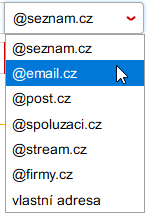
\includegraphics[width=1\textwidth]{selectChange.png}
			%\captionsetup{justification=justified, singlelinecheck=false}
			\caption{\texttt{<select>}}
			\label{subfig:selectChange}
		\end{subfigure}	
		\end{minipage}
	\hfill
	\begin{minipage}{0.45\textwidth}
		\begin{subfigure}[t]{1.0\textwidth}
			
\includegraphics[width=1\textwidth]{passwordChange.png}
			%	\captionsetup{justification=justified, singlelinecheck=false}
			\caption{\foreignlanguage{english}{\texttt{<input type="password">}}}
			\vspace{0.3cm}
			\label{subfig:passwordChange}
		\end{subfigure}	
	\vspace{0.3cm}
	\begin{subfigure}{1.0\textwidth}
		
\includegraphics[width=1\textwidth]{checkboxChange.png}
		\caption{\foreignlanguage{english}{\texttt{<input type="checkbox">}}}
		\label{subfig:checkboxChange}
	\end{subfigure}	
	\begin{subfigure}{1.0\textwidth}
		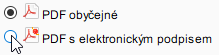
\includegraphics[width=1\textwidth]{radioChange.png}
		\caption{\foreignlanguage{english}{\texttt{<input type="radio">}}}
		\label{subfig:radioChange}
	\end{subfigure}
	\end{minipage}
	\caption{Několik elementů, jejichž změna hodnoty vyvolá událost "change"}
	\end{figure}
	Puppeteer nám dává k~dispozici metodu \texttt{select}, která umí vybrat hodnotu v~případě \subref{subfig:selectChange}. Pro přehrání vyťukání hesla v~\subref{subfig:passwordChange} existuje metoda \texttt{type} které můžeme nastavit i~volitelné zpoždění mezi jednotlivými údery.
	\begin{codefigure}[H]
	\begin{subfigure}[t]{\textwidth}
	\begin{lstlisting}[style=MyJavaScript]
page.select(selector, ...values)
	\end{lstlisting}
	\caption{}
	\end{subfigure}	
	\end{codefigure}
	\begin{codefigure}[H] \ContinuedFloat
		\begin{subfigure}[t]{\textwidth}
			\begin{lstlisting}[style=MyJavaScript]
page.type(selector, text, {delay: durationMs})
			\end{lstlisting}
			\caption{}
		\end{subfigure}
	\caption{Přehrávání události "change"}
	\end{codefigure}
	Pro poslední dva elementy \cref{subfig:checkboxChange} a~\ref{subfig:radioChange} je možné použít kliknutím, které je možné provést nám již známou metodou \texttt{click}. 
	\paragraph{Zápis/čtení textu do/ze schránky (události "copy" a~"paste")}
	Předtím, než se začneme zabývat kopírováním a~vkládáním, bychom rádi uvedli čtenáře do aktuálního stavu udělování oprávnění pomocí CDP, ať už nepřímo použítím Puppeteeru nebo nativně s~pouhým využítím CDP.
	
	Dle Puppeteer API by mělo být možné udělit oprávnění "push", nicméně při pokusu o~získání tohoto oprávnění je program ukončen s~výjimkou "Error: Unknown permission: push". Pro ověření tohoto tvrzení je možné spustit kód v~\ref{sub_sec:pushException}.
	
	S~oprávněními Pupppeteeru "clipboard-read" a~"clipboard-write" pro práci se schránkou je situace nápodobná jako u~oprávnění "push". Zřejmě bychom očekávali, že bez oprávnění "clipboard-read" ("clipboard-write") není možné číst (měnit) obsah schránky. Tak tomu ale není.
	
	Experimentálním ověřením s~nahlédnutím do zdrojového kódu Pupppeteeru a~online dokumentace CDP~\cite{devtoolsProtocol} jsme zjistili, že:
	\begin{itemize}[leftmargin=*]
		\item[--] Při neudělení žádného oprávnění je možné zapisovat do schránky, při pokusu o~čtení se zobrazí se zobrazí výzva pro udělení/neudělení oprávnění pro čtení. Připravený kód, kterým je možné toto ověřit se nachází v~\ref{sub_sec:accessClipboardWithoutPermission}.
		\item[--] Puppeteer nabízí oprávnění "clipboard-read" a~"clipboard-write", CDP definuje oprávnění "clipboardReadWrite" a~"clipboardSanitizedWrite". Při pokusu o~získání oprávnění "clipboard-read" nebo "clipboard-write" Puppeteer vždy zavolá CDP funkci \texttt{Browser.grantPermissions} s~parametrem \texttt{permissions} obsahující pouze "clipboardReadWrite".
		
		Volání této funkce, ať už přímo nativně nebo nepřímo s~použitím Puppeteeru, má za efekt to, že při pokusu zápisu do schránky se program ukončí s~výjimkou "Error: Evaluation failed: DOMException: Write permission denied.", více viz \ref{sub_sec:permissionsProblems}. Čtení naopak funguje bezproblémů viz \ref{sub_sec:readClipboardTest}. 
		\item[--] API Puppeteeru potažmo Puppeteer nijak nevyužívá oprávnění "clipboardSanitizedWrite" definované CDP, avšak udělením tohoto oprávnění získáme práva k~zápisu. Konečná funkční ukázka se nachází v~\ref{sub_sec:readingWritingClipboard}. 
	\end{itemize}
	Následující dvě tabulky shrnují chování.
	\nopagebreak
	\begin{table}[H]
		\centering
	%	\rowcolors{2}{alternatingRow}{white}
		\begin{tabular}{ l|l } 
			\rowcolor{tableHeadingBackground}
			\multicolumn{1}{l}{\textbf{Oprávnění CDP}} & \multicolumn{1}{l}{\textbf{Odpovídající oprávnění Puppeteeru}} \\
			\multirow{2}{*}{clipboardReadWrite} & clipboard-read \\ 
			& clipboard-write \\
			& \\
			clipboardSanitizedWrite & \strike{l}{}
		\end{tabular}
		\caption{Oprávnění pro schránku definované CDP a~Puppeteerem}
	\end{table}
	\begin{table}[H]
		\centering
%	\begin{longtable}{ lcc } 
	\begin{tabular}{ lcc }
		\rowcolor{tableHeadingBackground}
		\multicolumn{1}{l}{\textbf{Udělená oprávnění}} & \multicolumn{1}{l}{\textbf{Čtení}} & \multicolumn{1}{l}{\textbf{Zápis}} \\
		bez oprávnění & \xmark & \cmark \\
		clipboardReadWrite & \cmark & \xmark \\
		clipboardSanitizedWrite & \xmark & \cmark \\
		& & \\
		clipboardReadWrite & \multirow{2}{*}{\cmark} &  \multirow{2}{*}{\cmark} \\
		a~clipboardSanitizedWrite & &  \\
		\end{tabular}
%		clipboardReadWrite \newline a~clipboardSanitizedWrite & \cmark & \cmark 
	%\end{longtable}
	\caption{Skutečný význam oprávnění CDP pro schránku}
	\end{table}
	Důvodem těchto problémů může být, že online dokumentace CDP~\cite{devtoolsProtocol} uvádí celé API pro oprávnění jako experimentální.
	\section{Řešení}
	V~této kapitole se detailně zaměříme na vlastní řešení navržené s~využitím Puppeteeru. Začneme s~funkčními a~nefunkčními požadavky kladenými na naše řešení, od těch se přesuneme k~designu: popisu částí řešení a~způsobu komunikace mezi nimi, včetně diskuze o~vybraných technologiích. Poté se podíváme na funkčnost a~porovnáme ji vůči konkurenčním produktům. Dále v~této kapitole -- konkrétně v~\refAddedText{sub_sec:usersDocs}{části~}{} se nachází dokumentace pro uživatele. Pro zájemce o~detailnější popis implementace je připravena \refAddedText{sub_sec:programmerDocs}{podsekce }{}.
	\subsection{Požadavky}
	V~této části uvedeme specifikaci funkčních a~nefunkčních požadavků pro naše řešení. 
%	Číslování požadavků odpovídá formátu: 
%	\begin{center}
%		(PX TY)
%	\end{center}
%	\begin{itemize}
%		\item[--] X číslo požadavku.
%		\item[--] T typ požadavku, nabývá hodnot F pro funkční požadavek a N pro nefunkční požadavek.
%		\item[--] Y číslo požadavku v rámci jednoho typu požadavků.
%	\end{itemize}
	\subsubsection{Funkční} \phantom{}
	\vspace{-1.2cm}
	\begin{enumerate}[leftmargin=*, label={(F\arabic*)}]
		\item \label{item:recordingReq} \paragraph{Nahrávání (zaznamenání) akcí}
		Řešení musí podporovat nahrávání běžně prováděných úkonů v~prohlížeči. Za tyto úkony považujeme: kliknutí, přejetí myší přes element, vyplnění formuláře, odeslání formuláře, rolování a~načtení nové stránky.
		
		Mezi další úkony, které by mohly být podporovány patří: práce se \linebreak schránkou~--~kopírovaní a~vkládání, otevření nového tabu a~zavření existujícího tabu.
		\item \label{item:replayingReq} \paragraph{Přehrávání (znovuvykonání) akcí}
		Všechny akce, které je možné nahrát, musí být možné i~přehrát.
		\item \label{item:codeGenReq} \paragraph{Generování kódu}
		Řešení musí umožnit mimo okamžitého přehrávání i~vygenerovat skript, který je funkčně ekvivalentní s~přehráváním.
		\item \label{item:idReq} \paragraph{Použitelná identifikace elementů}
		Řešení musí podporovat nalezení různých identifikátorů elementu oproti běžně používaným (jednoznačná kombinace CSS tříd, argument id, absolutní popis cesty pomocí XPath, ...). 
		\item \label{item:connectionReq} \paragraph{Lokální i~vzdálené připojení k~prohlížeči}
		Kromě standardního vytvoření nové lokální instance prohlížeče, ve které jsou akce nahrávány nebo přehrávány, musí být možné se připojit i~na existující instanci spuštěnou na vzdáleném počítači.
		\item \label{item:settingsReq} \paragraph{Nastavení}
		Nahrávání a~přehrávání akcí bude konfigurovatelné, k~dispozici musí být alespoň nastavení: 
		\begin{itemize}
			\item[--] výběru typu akcí k~nahrávání
			\item[--] výběru akcí pro přehrávání
			\item[--] zpoždění akcí při přehrávání
			\item[--] specifik pro generování kódu (přidat řádky importující knihovny, ...)
		\end{itemize}
		\end{enumerate}
	\subsubsection{Nefunkční}
	Nefunkční požadavky odpovídající funkčním požadavkům mají vedle svého názvu uvedené číslo funkčního požadavku.
	\begin{enumerate}[leftmargin=*,label={(N\arabic*)}]
		%[\refstepcounter{enumi}(N\number\value{enumi} odp. F1-3)]
		\item \paragraph{Využití Pupppeteeru \normalfont{odp. \cref{item:recordingReq,item:replayingReq,item:codeGenReq}}}
		Implementace musí být provedena s~použitím knihovny Puppeteer, jedná se o~jádro práce, pro ostatní knihovny a~technologie existuje již mnoho automatizačních produktů viz \fullNameref{sub_sec:existingSolutions}.
		\item \paragraph{UI \normalfont{odp. \cref{item:recordingReq,item:replayingReq,item:codeGenReq,item:idReq,item:connectionReq,item:settingsReq}}}
		Celé řešení bude možné ovládat z~uživatelského rozhraní.
		\item \paragraph{Kompatibilita napříč platformami}
		Technologie pro implementaci musí být zvoleny tak, aby byla zajištěna kompatibilita alespoň s~OS Windows a~Linux.
	\end{enumerate}
	\subsection{Design}
	\label{sub_sec:design}
	Řešení se skládá ze dvou celků. Prvním je knihovna pro přehrávání a~nahrávání akcí vytvořená s~běhovým prostředím Node.js v~JavaScriptu, dále označovaná jako backend. Vzhledem k~implementaci Puppeteeru v~TypeScriptu\footnote{JavaScript se statickým typováním spravovaný firmou Microsoft~\cite{typeScript}.} jsme se rozhodli pro JavaScript. Druhým celkem je okenní WinForms aplikace implementovaná v~C\# pro poskytnutí UI, tu nazveme frontend. C\# a~WinForms jsme vybrali z~těchto důvodů:
	\begin{enumerate}[leftmargin=*]
		\item \paragraph{Jednoduchost}
		Jak uvádí dokumentace firmy Microsoft~\cite{csharpHistory}, která stojí za vznikem C\#, jedním z~designových cílů již od verze 1.0 byla snaha o~"jednoduchý, moderní, univerzální objektově orientovaný jazyk". Stejně jako C\# i~návrh UI ve WinForms považujeme za jednoduchý, a~to zejména díky obrovskému množství již existujících komponent (ProgressBar, PropertyGrid, ...) a~vývoji pomocí drag and drop. Cílem této práce není vytvářet UI podle grafického návrhu a~navíc WinForms obsahuje většinu námi potřebných komponent\footnote{Chybí pouze textový editor se zvýrazňováním syntaxe, a~tak využijeme externí viz \ref{docs:codeGenEditor}, \ref{docs:jsonEditor}.} a~všechny nutné funkce.
		\item \paragraph{Přenositelnost}
		Jazyk C\# byl vydán s~vývojovým prostředím Visual Studio .NET 2002~\cite{csharpHistory}, současná verze Visual Studio 2019 je stále  kompatibilní pouze s~Windows~\cite{visualStudioMainPage}, zatímco programy vytvořené v~C\# s~WinForms je možné spouštět i~na jiných platformách (Linux, macOS, BSD a~další), díky projektu Mono\footnote{Multiplatformní implementace .NET Framework s~otevřeným zdrojovým kódem~\cite{monoProject}.}~\cite{monoProject}.
		\item \paragraph{Vyzrálost}
		Součástí první verze .NET Framework vydané v~únoru 2002 byl WinForms. Dnes je stále její součástí, ač je tomu nyní již 19 let. O~výběru technologie pro UI by se jistě dalo diskutovat -- pouze samotný Microsoft stihl vydat WPF a~UWP, WPF slouží výhradně pro vývoj UI~\cite{wpfDocs} a~UWP je, spolu s~vývojem UI, přímo univerzální platforma pro vývoj Windows aplikací~\cite{uwpDocs}. Narozdíl od WinForms, WPF i~UWP fungují pouze na Windows\footnote{WPF (Windows Presentation Foundation) vyžadují ke svému běhu .NET Framework 3.0, jeho otevřená implementace Mono sice na svém webu deklaruje kompatibilitu s~verzí 4.7, explicitně však uvádí, že WPF nepodporuje~\cite{monoCompatibility}.
			
			UWP (Universal Windows Platform) je z~hlediska osobních počítačů dle oficiální dokumentace~\cite{uwpSupportedPlatforms} kompatibilní pouze s~Windows~10.
		}. 
		
		
		Na Internetu se často vyskytují otázky týkající se končícího životního cyklu WinForms~\cite{winformObselote1,winformsObselote2,winformsObselote3, winformsObselote4, winformsObselote5}. Místo souhlasu s~tím, že WinForms jsou mrtvé, se domníváme, že jejich stáří přispívá ke stabilitě a~neměnosti API, které může i~způsobit ztrátu kompatibility mezi jednotlivými verzemi.
		
%		Často vyskytujícími se otázkami na Internetu probírající docházející životní cyklus WinForms  Místo souhlasu s~často vyskytujícími se otázkami na Internetu, že WinForms jsou mrtvé~\cite{winformObselote1,winformsObselote2,winformsObselote3, winformsObselote4, winformsObselote5} se domníváme, že jejich stáří přispívá ke stabilitě a~neměnosti API, které může i~způsobit ztrátu kompatibility mezi jednotlivými verzemi.
	\end{enumerate}
	Backend a~frontend mezi sebou potřebují vzájemně komunikovat. Např. frontend spouští nahrávání, tj. odesílá pokyn ke spuštění nahrávání backendu. Naopak backend při nahrávání ohlašuje zachycenou událost do frontendu. Pro komunikaci mezi dvěma procesy bychom mohli využít BSD sockety, které mají nativní podporu v~API Node.js~\cite{nodejsApi} i~v~API .NET Frameworku~\cite{dotnetApi}, avšak pro tyto účely již existuje řada knihoven. 
	
	Vybrali jsme knihovnu ZeroMQ~\cite{zeromq} pro tyto její výhody:
	\begin{itemize}
		\item[--] Existence mnoha nativních portů, případně language bindingů pro spoustu jazyků~\cite{zeromqDocs}. Pro nás zásadní je existence portu NetMQ~\cite{netmqGithub} pro C\#\footnote{Existuje i~binding clrzmq4~\cite{crlzmq4}, dokumentace~\cite{zeromqCSharp} ale doporučuje použít NetMQ.} a~bindingu ZeroMQ.js~\cite{zeromqJs} pro JavaScript.
		\item[--] ZeroMQ nevyžaduje message broker, vrstvu mezi frontendem a~backendem zpracovávající zprávy~\cite{messageBroker} viz \ref{sub_sec:zeromqDemo}.
		\item[--] Jednoduché API umožňující přímé odeslání zpráv jako textových řetězců viz~\ref{sub_sec:zeromqDemo}.
	\end{itemize}
	Design řešení včetně jeho částí a~komunikace mezi frontendem a~backendem ilustruje následující diagram.
	\nopagebreak
	\begin{figure}[H]
		\centering
		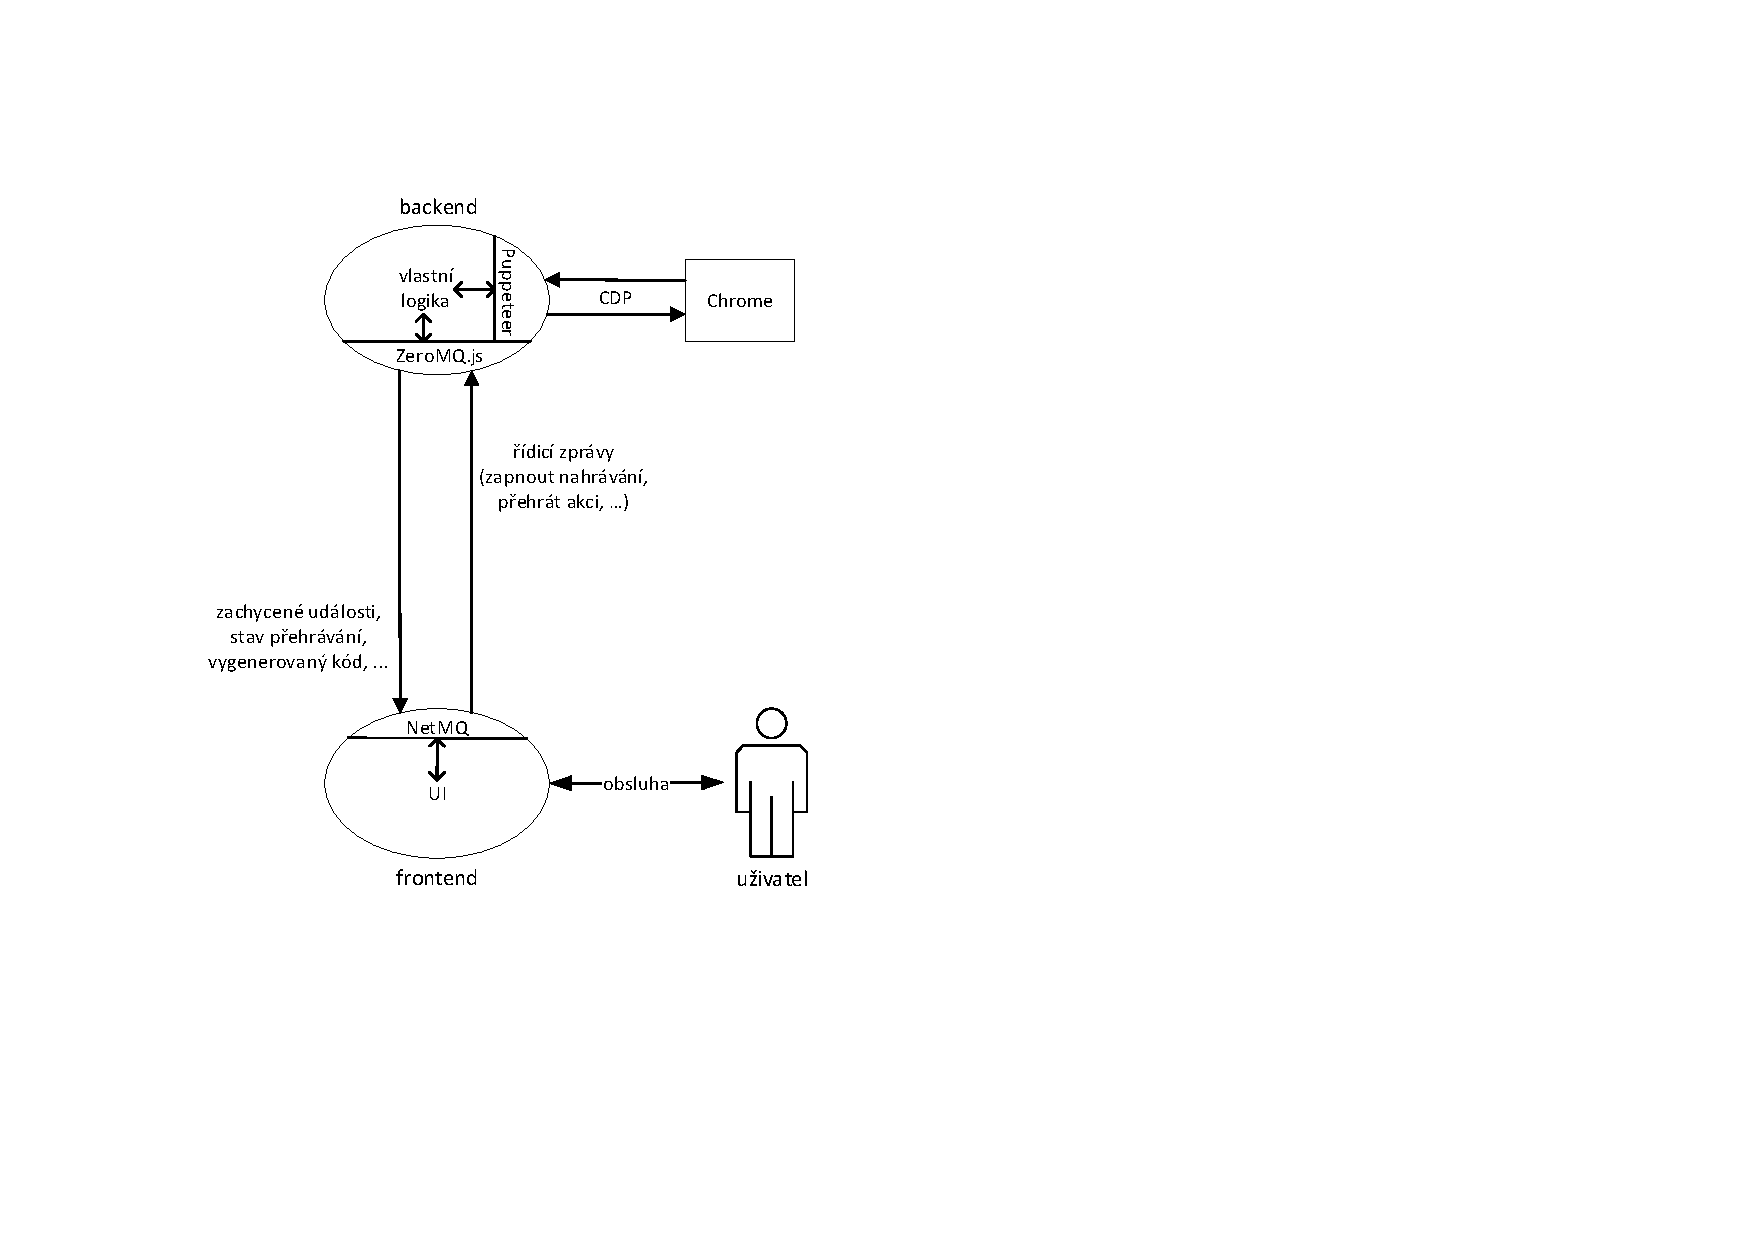
\includegraphics[width=0.8\textwidth]{design.pdf}
		\caption{Diagram řešení}
	\end{figure}
	\newpage
	\subsection{Scénáře použití}
	V~této části bude následovat několik diagramů, které ilustrují možnosti uživatelů pro využití řešení.
	\paragraph{Hlavní okno}
	Hlavní okno reprezentuje stav ihned po spuštění.
	\begin{figure}[H]
		\centering
		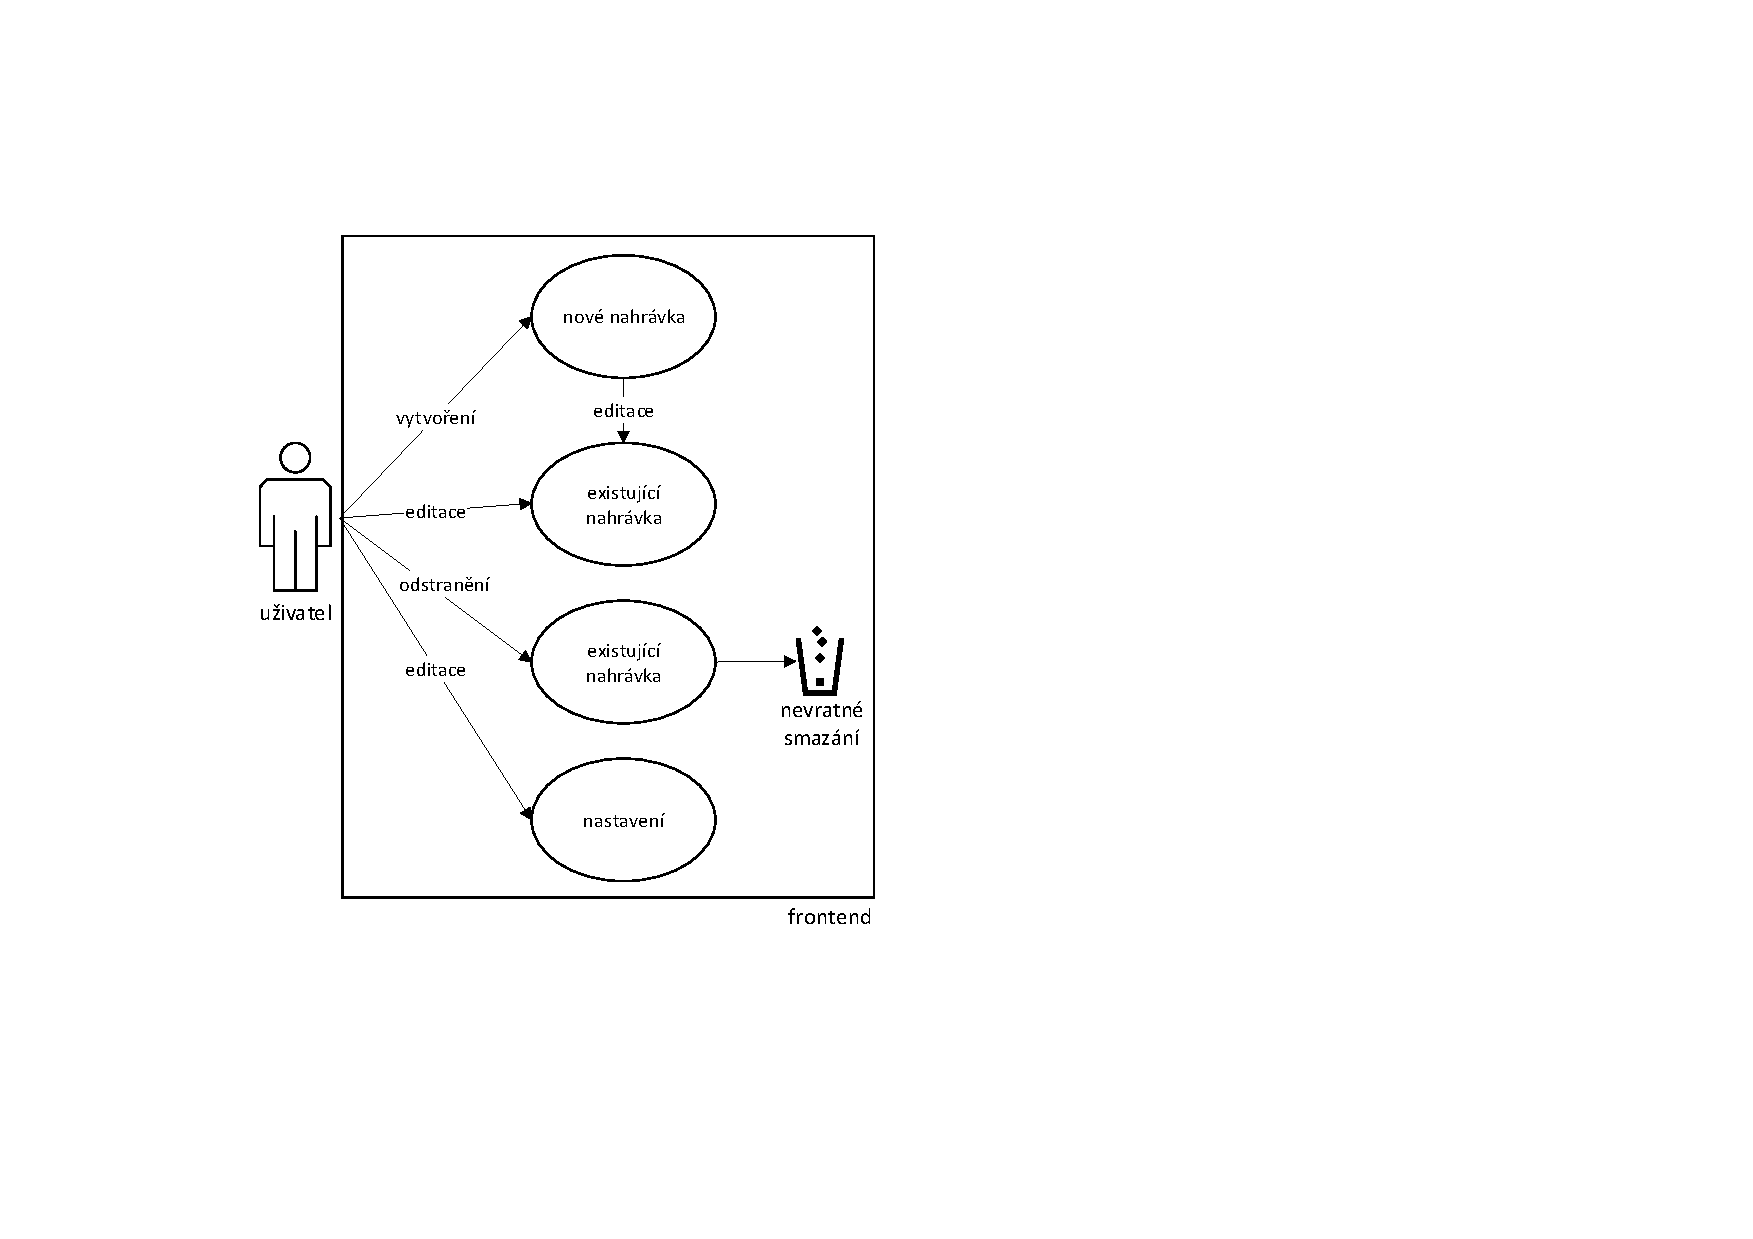
\includegraphics[width=0.8\textwidth]{mainWindowDiagram.pdf}
		\caption{Diagram hlavního okna}
	\end{figure}
	\paragraph{Editace existujícího nahrávky}
	Zde rozvedeme konkrétní možnosti pro editaci existující nahrávky.
	\nopagebreak
	\begin{figure}[H]
		\hspace{0.3cm}
		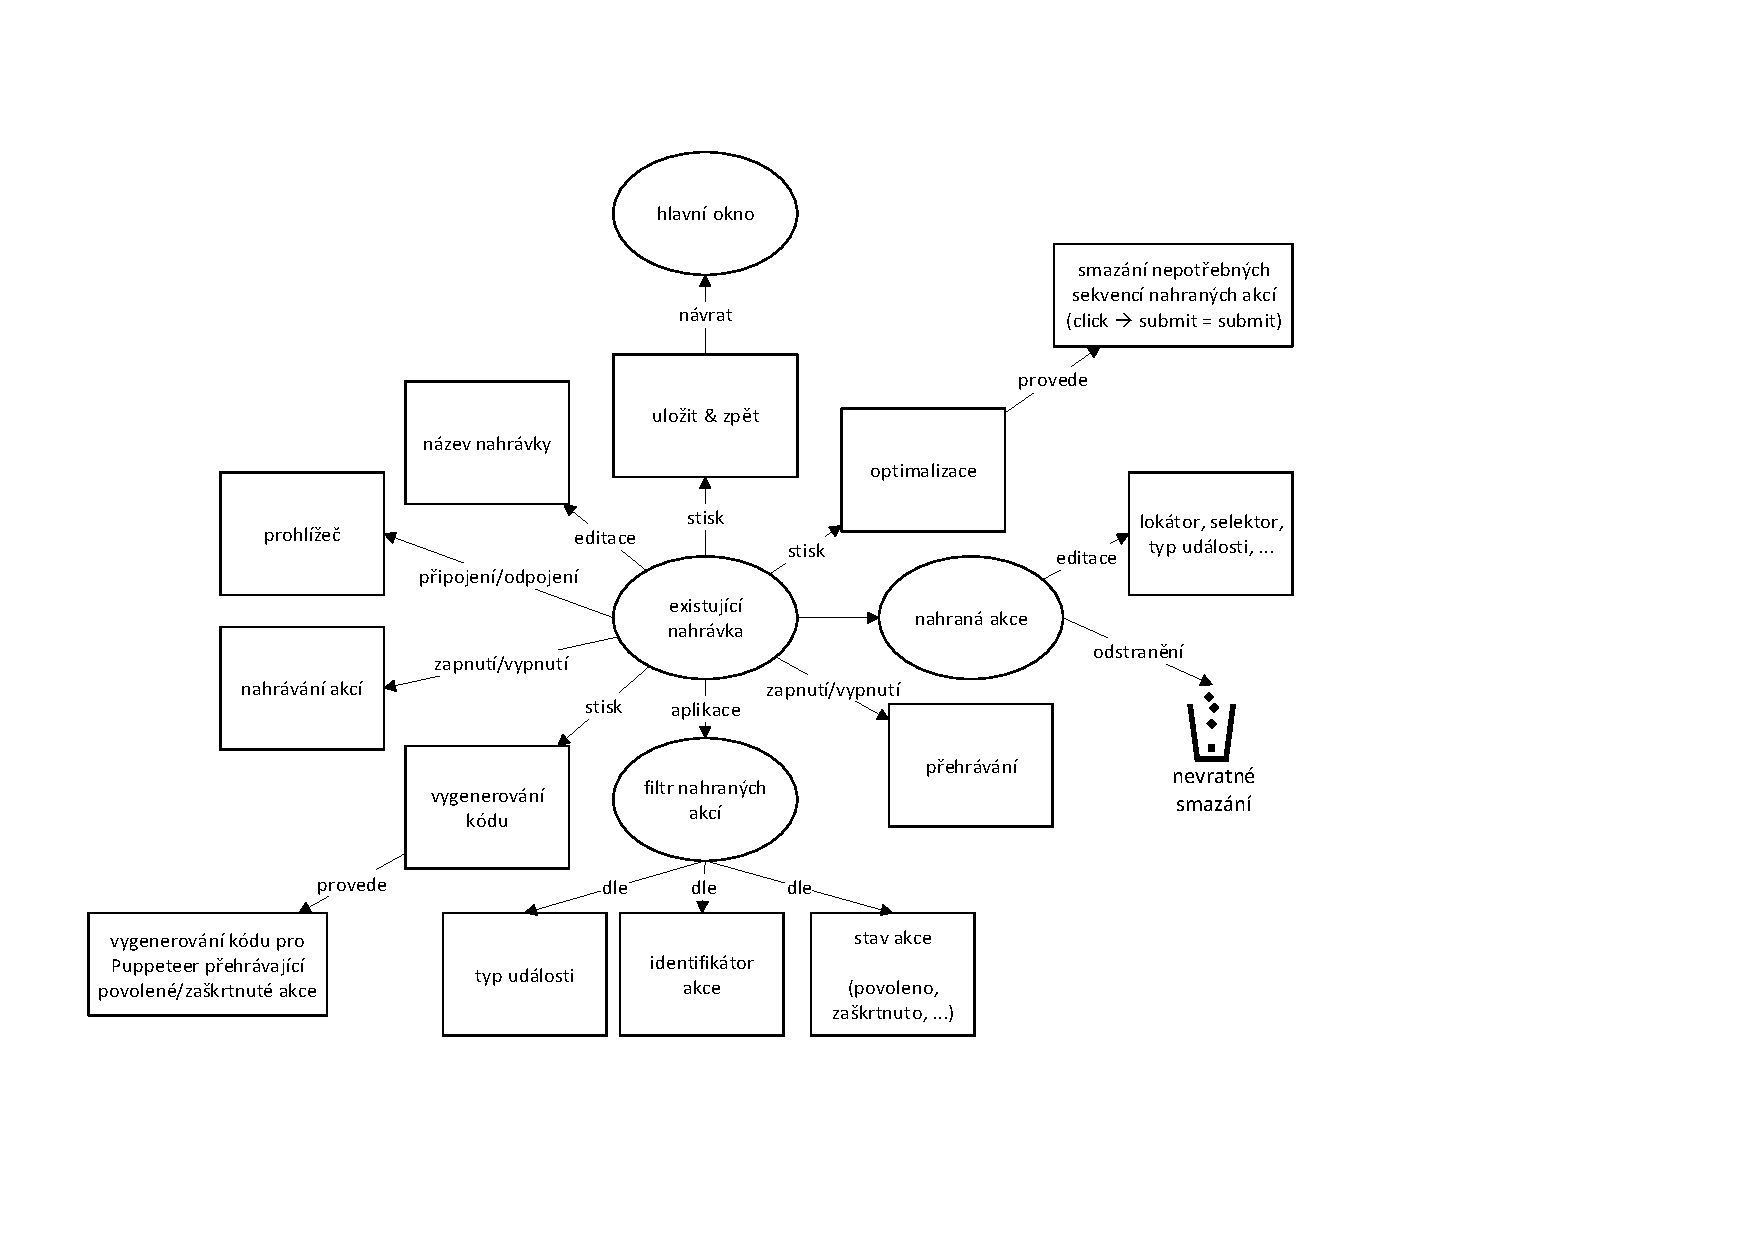
\includegraphics[width=1.3\textwidth, center]{recordingEditDiagram.pdf}
%	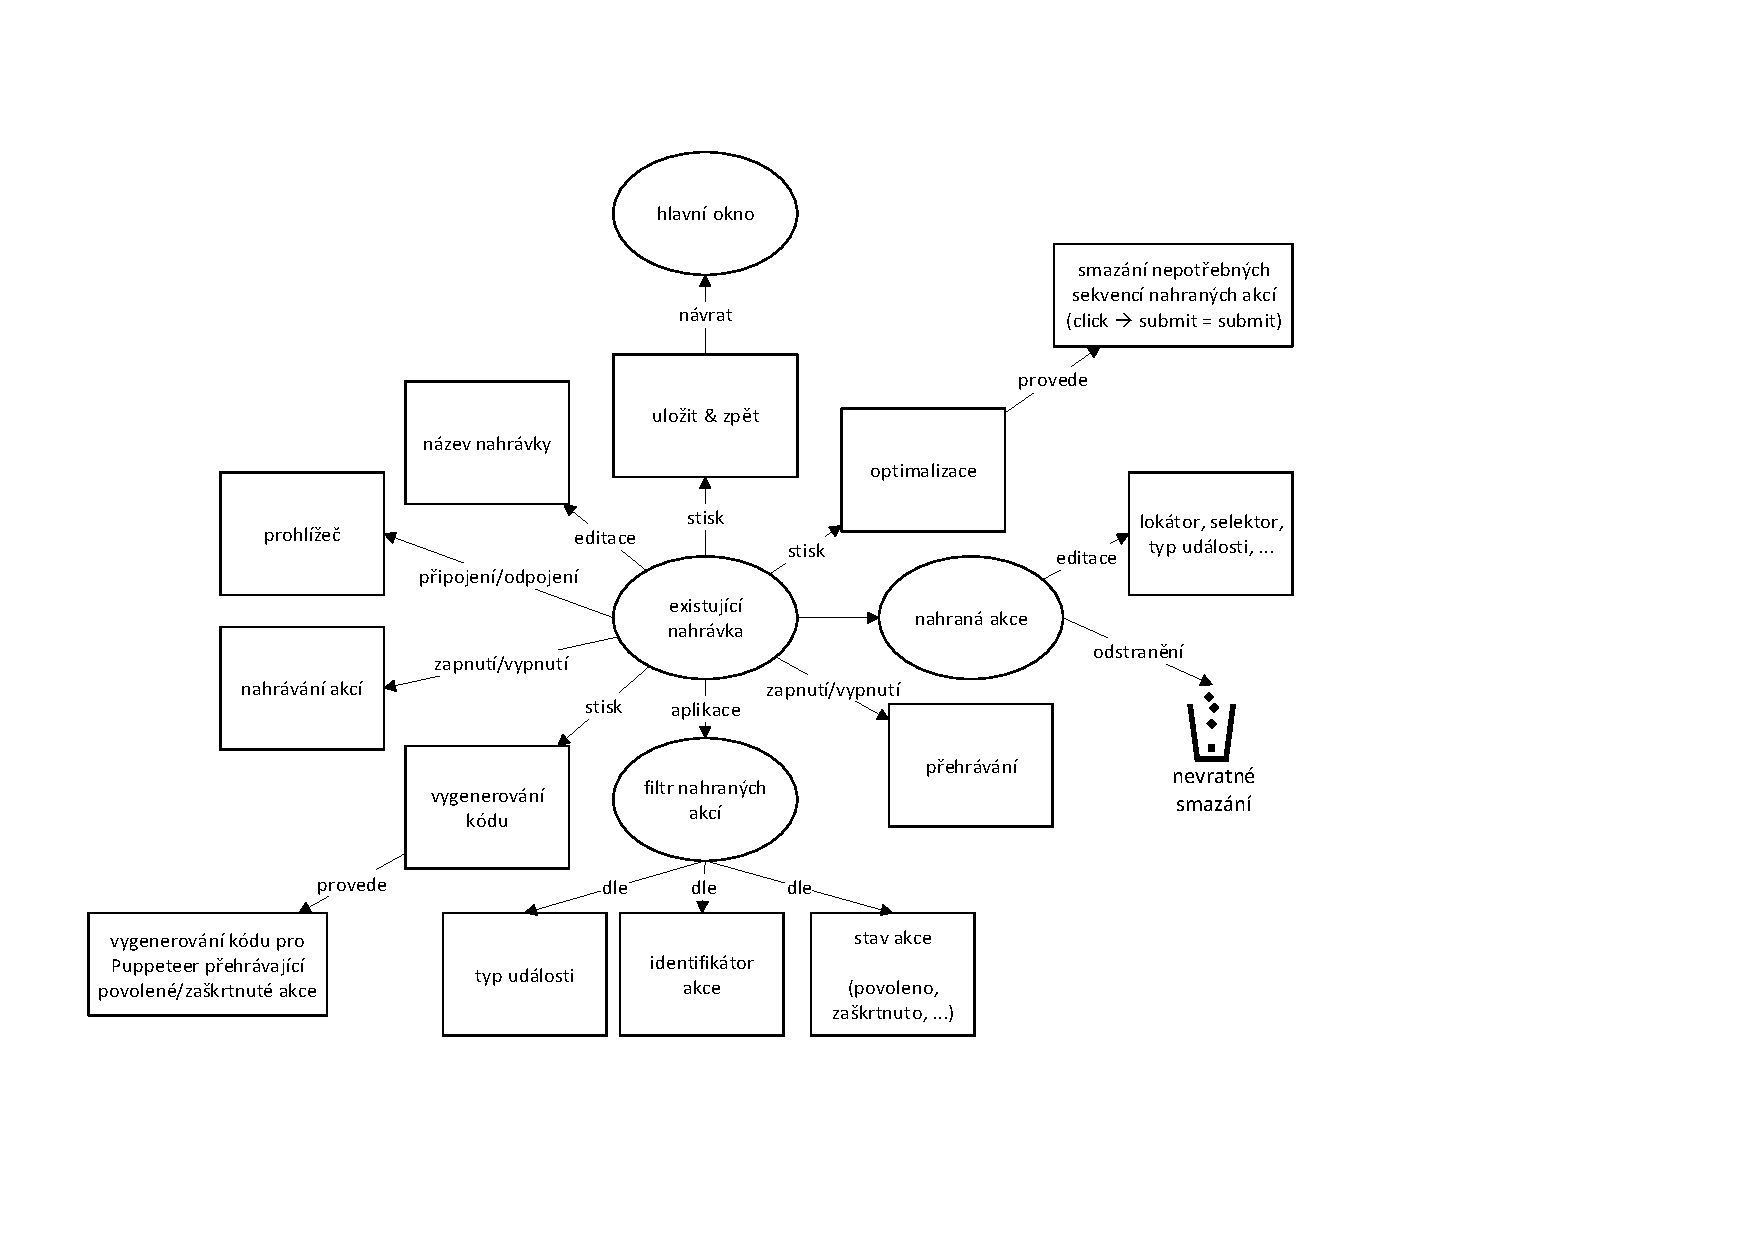
\includegraphics[angle=90, origin=c,width=1.0\textwidth]{recordingEditDiagram.pdf}
	\caption{Diagram editace existující nahrávky}
	\end{figure}
	\paragraph{Editace nastavení}
	Nyní si ukážeme některé konkrétní možnosti editace nastavení.
	\nopagebreak
	\begin{figure}[H]
		\centering
		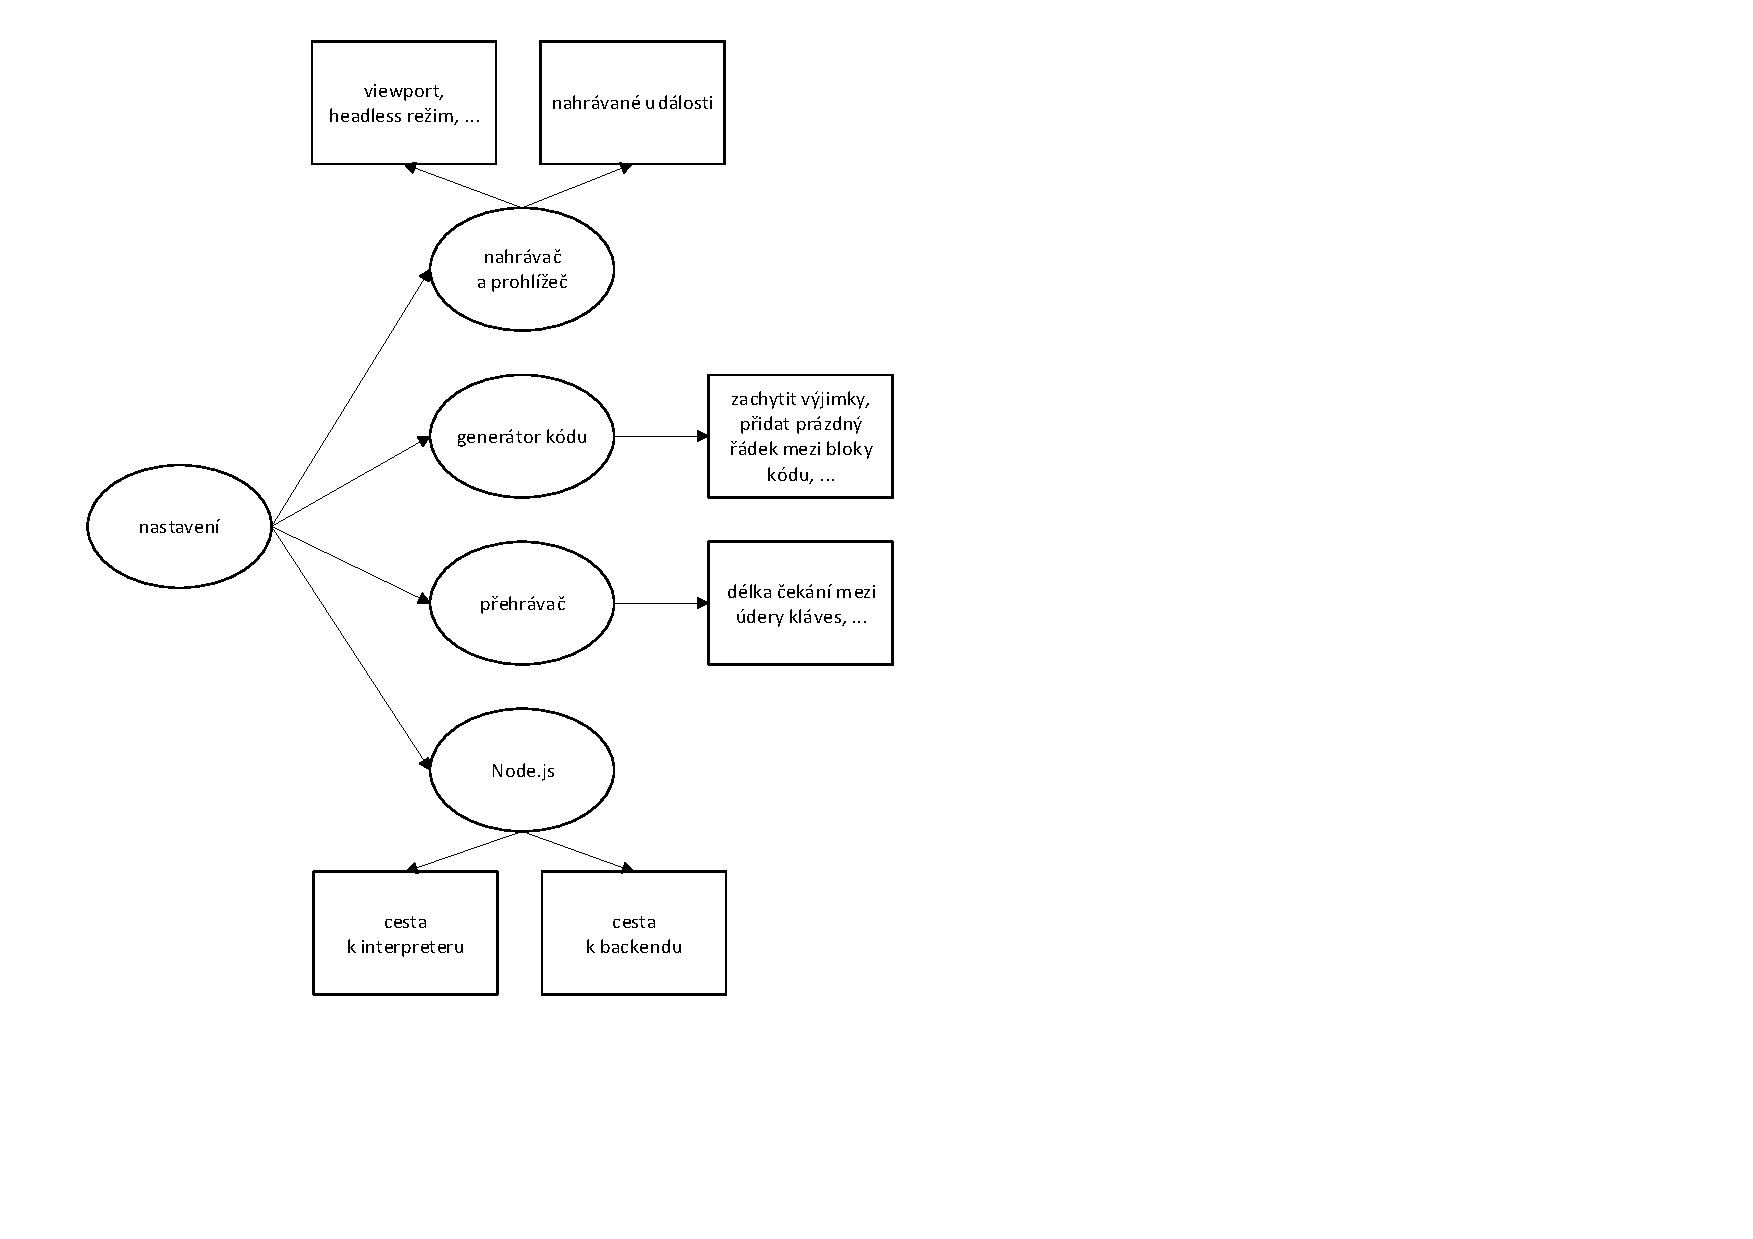
\includegraphics[width=1.0\textwidth]{settingsDiagram.pdf}
		\caption{Diagram editace nastavení}
	\end{figure}
	\newpage
	\subsection{Porovnání funkcionality oproti konkurenčním řešením}
	\label{sub_sec:functionalityComparison}
	Ještě předtím než začneme porovnávat bychom rádi upozornili na zásadní odlišující faktor vlastního řešení, a~sice využití Puppeteeru. Ostatní řešení zmíněná v~této práce využívala Selenium, případně byla proprietární. (Výjimkou je Headless Recorder, ten je postavený nad Puppeteerem, ale neumí přehrávání -- nepovažujeme ho za plnohodnotné řešení.)
	\paragraph{Události viewportu}
{
	\rowcolors{2}{alternatingRow}{white}  
%	\setlength\LTleft{-3cm}
%	\setlength\LTright{-3cm}
	\begin{longtable}{ l|C{2.0cm}|C{2.0cm}|C{2.0cm}|C{1.9cm}|C{1.7cm} } 
		\rowcolor{tableHeadingBackground} 
		\multicolumn{1}{l}{\textbf{Událost}} &
		\multicolumn{1}{p{2.0cm}}{\textbf{Selenium IDE}} & \multicolumn{1}{p{2.0cm}}{\textbf{Katalon Recorder}} & \multicolumn{1}{p{2.0cm}}{\textbf{Ranorex Recorder}} & \multicolumn{1}{p{1.9cm}}{\textbf{Headless Recorder}} & \multicolumn{1}{p{1.7cm}}{\textbf{Vlastní řešení}} \\
		 click & \cmark  & \cmark  & \cmark & \cmark & \cmark \\
		 dblclick & \cmark  & \cmark  & \cmark & vygeneruje kód pro 2x~click & \cmark \\
    	 input &  \cmark & \cmark & \cmark & \cmark & \cmark \\		 		 
    	 change  & \cmark & \cmark & \cmark & \cmark & \cmark \\
    	 select & \xmark  & \xmark  & provádí relativní pohyb kurzoru simulující výběr textu & \xmark & \cmark \\
    	 submit & \cmark  & \cmark & provede akci spouštějící submit & provede akci spouštějící submit & \cmark \\
    	 scroll & \cmark & \xmark & \cmark & \xmark & \cmark \\
    	 copy, paste & pracuje s~vlastní interní schránkou & pracuje s~vlastní interní schránkou & \cmark & \xmark & \cmark \\
    	 mouseover & pomocí kontextové nabídky & \xmark & simulace pohybu kurzoru & \xmark & podržením klávesy 'h' \\
    	 \rowcolor{white}
		\caption{Porovnání podporovaných událostí viewportu napříč řešeními}
	\end{longtable}
}
	\newpage
	\paragraph{Události okna prohlížeče}
	%otevření nového tabu, uzavření existujícího tabu, změna url adresy, změna aktivního tabu
{
	\rowcolors{2}{alternatingRow}{white}  
	%	\setlength\LTleft{-3cm}
	%	\setlength\LTright{-3cm}
	\begin{longtable}{ p{2.5cm}|C{2.0cm}|C{1.7cm}|C{1.7cm}|C{1.7cm}|C{2.0cm} } 
		\rowcolor{tableHeadingBackground} 
		\multicolumn{1}{p{2.5cm}}{\textbf{Událost}} &
		\multicolumn{1}{p{2.0cm}}{\textbf{Selenium IDE}} & \multicolumn{1}{p{1.7cm}}{\textbf{Katalon Recorder}} & \multicolumn{1}{p{1.7cm}}{\textbf{Ranorex Recorder}} & \multicolumn{1}{p{1.7cm}}{\textbf{Headless Recorder}} & \multicolumn{1}{p{2.0cm}}{\textbf{Vlastní\newline řešení}} \\
		otevření nového tabu & implicitně s~akcí elementu  & implicitně s~akcí elementu & \cmark & \xmark & \cmark \\
		uzavření existujícího tabu & \cmark  & \cmark & \cmark & \xmark & \xmark \\
		změna URL~adresy & ručním přidáním akce open  & ručním přidáním akce open  & \cmark & \xmark & \cmark \\
		změna\newline aktivního tabu & \cmark & \cmark & \cmark & \xmark & detekováno s~následující událostí \\
		\rowcolor{white}
		\caption{Porovnání podporovaných událostí okna prohlížeče napříč řešeními}
	\end{longtable}
}	
	\paragraph{Identifikátory elementů}
{
%	\rowcolors{2}{alternatingRow}{white}  
	%	\setlength\LTleft{-3cm}
	%	\setlength\LTright{-3cm}
	\begin{longtable}{ p{2.0cm}|C{1.5cm}|C{1.7cm}|C{3.0cm}|C{1.7cm}|C{1.7cm} } 
		\rowcolor{tableHeadingBackground} 
		\multicolumn{1}{p{2.0cm}}{\textbf{Typ identifikátoru}} &
		\multicolumn{1}{p{1.5cm}}{\textbf{Selenium IDE}} & \multicolumn{1}{p{1.7cm}}{\textbf{Katalon Recorder}} & \multicolumn{1}{p{3.0cm}}{\textbf{Ranorex\newline Recorder}} & \multicolumn{1}{p{1.7cm}}{\textbf{Headless Recorder}} & \multicolumn{1}{p{1.7cm}}{\textbf{Vlastní\newline řešení}} \\
		selektory & \cmark & \xmark & \newline \multirow{2}{3.0cm}{využivá proprietárně rozšířený xpath identifikující i~mimo viewport} & \cmark & \cmark \\
		& & & & & \\
		lokátory & \cmark & pouze id, name, xpath & & \xmark & \cmark \\
		\rowcolor{white}
		\caption{Porovnání podporovaných identifikátorů elementů napříč řešeními}
	\end{longtable}
}
	\newpage
	\paragraph{Čekání na}
{
		\rowcolors{2}{alternatingRow}{white}  
	%	\setlength\LTleft{-3cm}
	%	\setlength\LTright{-3cm}
	\begin{longtable}{ p{1.7cm}|C{1.7cm}|C{1.7cm}|C{1.7cm}|C{1.7cm}|C{1.7cm} } 
		\rowcolor{tableHeadingBackground} 
		\multicolumn{1}{p{1.7cm}}{\textbf{Čekání na}} &
		\multicolumn{1}{p{1.7cm}}{\textbf{Selenium IDE}} & \multicolumn{1}{p{1.7cm}}{\textbf{Katalon Recorder}} & \multicolumn{1}{p{1.7cm}}{\textbf{Ranorex\newline Recorder}} & \multicolumn{1}{p{1.7cm}}{\textbf{Headless Recorder}} & \multicolumn{1}{p{1.7cm}}{\textbf{Vlastní\newline řešení}} \\
		existenci elementu & \cmark & \cmark & \cmark & \cmark & \cmark \\
		hodnotu atributu elementu & \xmark & \cmark & \cmark & \xmark & \xmark \\
		možnost editace elementu & \cmark & \cmark & \cmark & \xmark & \xmark \\
		dokončení navigace & implicitní čekání na zavolání události 'load' & implicitní čekání na zavolání události 'load' & \cmark & implicitní čekání na zavolání události 'load' & \cmark \\
		viditelnost elementu & \cmark & \cmark & \cmark & \xmark & \xmark \\
		\rowcolor{white}
		\caption{Porovnání podporovaných druhů čekání napříč řešeními}
	\end{longtable}
}
	\paragraph{Možnosti exportu}
{
		\rowcolors{2}{alternatingRow}{white}  
	%	\setlength\LTleft{-3cm}
	%	\setlength\LTright{-3cm}
%	{\renewcommand*\arraystretch{2.7}} 
	\begin{longtable}{ C{2.7cm}|C{1.5cm}|C{1.7cm}|C{1.7cm}|C{1.7cm}|C{1.7cm} }
		\rowcolor{tableHeadingBackground} 
		\multicolumn{1}{p{2.7cm}}{\textbf{Technologie}} &
		\multicolumn{1}{p{1.5cm}}{\textbf{Selenium IDE}} & \multicolumn{1}{p{1.7cm}}{\textbf{Katalon Recorder}} & \multicolumn{1}{p{1.7cm}}{\textbf{Ranorex\newline Recorder}} & \multicolumn{1}{p{1.7cm}}{\textbf{Headless Recorder}} & \multicolumn{1}{p{1.7cm}}{\textbf{Vlastní\newline řešení}} \\
		C\# (MSTest) & \xmark & \cmark & \xmark & \xmark & \xmark \\
		C\# (NUnit) & \cmark & \cmark & \xmark & \xmark & \xmark \\
		C\# (xUnit) & \cmark & \xmark & \xmark & \xmark & \xmark \\
		Java (JUnit) & \cmark & \cmark & \xmark & \xmark & \xmark \\
		JavaScript (Mocha) & \cmark & \xmark & \xmark & \xmark & \xmark \\
		JavaScript (New Relic Synthetics) & \xmark & \cmark & \xmark & \xmark & \xmark \\
		JavaScript (Playwright) & \xmark & \xmark & \xmark & \cmark & \xmark \\
		JavaScript (Puppeteer) & \xmark & \xmark & \xmark & \cmark & \cmark \\
		JavaScript (WebDriver.io) & \xmark & \cmark & \xmark & \xmark & \xmark \\
		JSON & \xmark & \cmark & \xmark & \xmark & \xmark \\
		Katalon Studio & \xmark & \cmark & \xmark & \xmark & \xmark \\
		mezikód pro výrobu nových formáterů & \xmark & \cmark & \xmark & \xmark & \xmark \\
		Python (AppDynamics) & \xmark & \cmark & \xmark & \xmark & \xmark \\
		Python (pytest) & \cmark & \xmark & \xmark & \xmark & \xmark \\
		Python 2 (unittest) & \xmark & \cmark & \xmark & \xmark & \xmark \\
		Robot Framework & \xmark & \cmark & \xmark & \xmark & \xmark \\
		Ruby RSpec & \cmark & \cmark & \xmark & \xmark & \xmark \\
		samostatný spustitelný soubor & \xmark & \xmark & \cmark & \xmark & \xmark \\
		TypeScript (Protractor) & \xmark & \cmark & \xmark & \xmark & \xmark \\
		XML & \xmark & \cmark & \xmark & \xmark & \xmark \\
		\rowcolor{white}
		\caption{Porovnání podpory generování kódu napříč řešeními}
	\end{longtable}
}
\newpage
	\paragraph{Další pokročilé funkce}
{
	\rowcolors{2}{alternatingRow}{white}  
	%	\setlength\LTleft{-3cm}
	%	\setlength\LTright{-3cm}
	%	{\renewcommand*\arraystretch{2.7}} 
	\begin{longtable}{ C{2.7cm}|C{1.5cm}|C{1.7cm}|C{2.0cm}|C{1.7cm}|C{1.7cm} }
		\rowcolor{tableHeadingBackground} 
		\multicolumn{1}{p{2.7cm}}{\textbf{Funkce}} &
		\multicolumn{1}{p{1.5cm}}{\textbf{Selenium IDE}} & \multicolumn{1}{p{1.7cm}}{\textbf{Katalon Recorder}} & \multicolumn{1}{p{2.0cm}}{\textbf{Ranorex\newline Recorder}} & \multicolumn{1}{p{1.7cm}}{\textbf{Headless Recorder}} & \multicolumn{1}{p{1.7cm}}{\textbf{Vlastní\newline řešení}} \\
		větvení (podmínky) & if, else~if, else & if,\linebreak else~if, else & možnost propojení s~~C\# & \xmark & \xmark \\
		cykly & do, times, while, foreach & while & možnost propojení s~~C\# & \xmark & \xmark \\
		zvýraznění identifikovaného elementu uvnitř viewportu  & \cmark & \cmark & dokonce i~streamování aktuální podoby elementu & \xmark & \xmark \\
		změna elementu existující akce klikem uvnitř viewportu & \cmark & \cmark & pomocí sofistikované součásti Ranorex Spy & \xmark & ruční změna nebo nahrání nové akce \\
		ruční přidání akce & \cmark & \cmark & \cmark & \xmark & \xmark \\
		nastavení velikosti viewportu & \cmark & \xmark & \cmark & \xmark & bez dynamických změn během nahrávání \\
		volitelné zpomalení přehrávání & \cmark & \cmark & \cmark & \xmark & \cmark \\
		připojení na vzdálený prohlížeč & \xmark & \xmark & pouze přehrávání přes RDP  & \xmark & \cmark \\
		\rowcolor{white}
		\caption{Porovnání dalších pokročilých funkcí napříč řešeními}
	\end{longtable}
}
	\newpage
	\subsection{Tutoriály}
	\label{sub_sec:usersDocs}
	Nyní se podívame na UI frontendové části přes kterou se naše řešení ovládá. Využití uživatelského rozhraní bude demonstrováno několika tutoriály.
	
	Tutoriály jsou vytvořené tak, aby ukazovaly základní funkcionalitu řešení, případně vysvětlovali neintuitivní části UI. Velká část zřejmých komponent UI je vynechána pro přehlednost v~dokumentaci.
	 %Součástí uživatelské příručky je i podsekce chybových hlášek \ref{subsub_sec:troubleshooting} obsahující jejich důvod a řešení.
	\subsubsection{Prvotní spuštění}
	\label{subsub_sec:firstRun}
	
	Pro správnou funkci je nutné určit typ připojení ke~Chromu, nastavit cestu k~interpreteru Node.js pokud není umístěna v~proměnné Path proměnného prostředí. Jestliže byla změněna relativní cesta backendu vůči frontendu, tak je nutné nastavit novou cestu i~k~backendu. Začneme připojením Chromu.
	\begin{figure}[H]
		\centering
		\begin{minipage}{0.49\textwidth}
			\begin{subfigure}[t]{1.0\textwidth}
				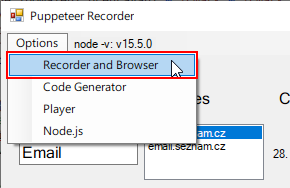
\includegraphics[width=1.0\textwidth]{recorderSettingsMenuItem.png}
			\end{subfigure}	
		\end{minipage}
		\hfill
		\textrightarrow
		\hfill
		\begin{minipage}{0.45\textwidth}
			\begin{subfigure}[t]{1.0\textwidth}
				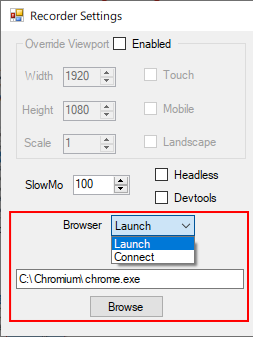
\includegraphics[width=1.0\textwidth, right]{chromeConnection.png}
			\end{subfigure}	
		\end{minipage}
		\caption{Nastavení připojení ke~Chromu}
		\label{fig:chromeConnection}
	\end{figure}
	Jak je patrné z~\cref{fig:chromeConnection}, na výběr máme ze dvou typů připojení. "Launch" spustí novou lokální instanci Chromu, volitelně vyžaduje zadání cesty ke spustitelnému souboru prohlížeče, její zadání je nutné pokud se spustitelný soubor Chromu nenachází ve standardním umístění. Druhý typ připojení označený jako "Connect" se připojí k~existující vzdálené instanci Chromu, více o~tomto druhu připojení viz \refFullAddedText{subsub_sec:remoteChrome}{tutoriál }{}.
	
	Poslední dvě zbývající cesty pro backend a~Node.js se nastavují ve společném dialogovém okně.
	\begin{figure}[H]
		\centering
		\begin{minipage}{0.47\textwidth}
			\begin{subfigure}[t]{1.0\textwidth}
				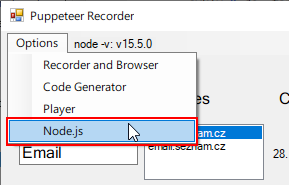
\includegraphics[width=1.0\textwidth]{nodejsSettings.png}
			\end{subfigure}	
		\end{minipage}
		\hfill
		\textrightarrow
		\hfill
		\begin{minipage}{0.47\textwidth}
			\begin{subfigure}[t]{1.0\textwidth}
				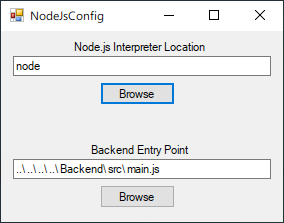
\includegraphics[width=1.0\textwidth, right]{nodejsSettings2.png}
			\end{subfigure}	
		\end{minipage}
		\caption{Nastavení cesty k~interpreteru Node.js a~backendu}
	\end{figure}
	Obě vyplněné cesty jsou výchozí hodnotou nastavení. Všimněme si, že jako cesta k~interpreteru Node.js stačí uvést pouze "node" pokud je jeho umístění v~proměnné Path proměnného prostředí. 
	
	Cesta k~backendu je popsána relativně vůči umístění spustitelného souboru frontendové části. Pokud nebyla upravena struktura projektu, cesta k~backendu je správná.
	\subsubsection{Nová nahrávka}
	Zkusíme si vytvořit jednoduchou nahrávku na~které si ukážeme základní součásti editačního UI pro nahrávky. 
	\begin{figure}[H]
		\centering
		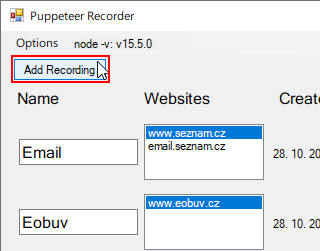
\includegraphics[width=0.58\textwidth]{addNewRecording.png}
		\caption{Vytvoření nové nahrávky}
		\label{fig:addNewRecording}
	\end{figure}
	\newpage
	Po stisknu zvýrazněného tlačítka na \cref{fig:addNewRecording} se změní podoba okna pro nahrávání a~přehrávání akcí, okno bude vypadat takto:
	\begin{figure}[H]
		\centering
		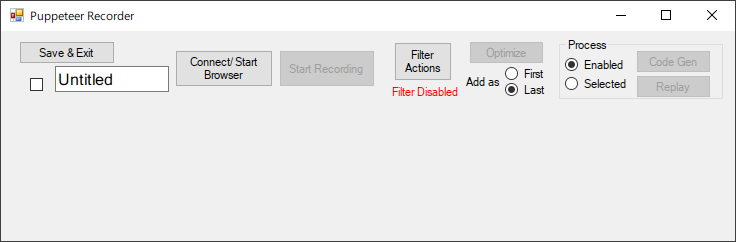
\includegraphics[width=1.0\textwidth]{emptyRecordingEdit.png}
		\caption{Editační UI pro nahrávky}
	\end{figure}
	Nyní máme prázdnou nahrávku, naším cílem bude nahrát několik akcí, přehrát je a~zobrazit si jejich kód pro Puppeteer. Předtím však však změníme jméno nahrávky z~"Untitled" na "První nahrávka".
	\begin{figure}[H]
		\centering
		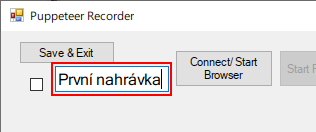
\includegraphics[width=0.57\textwidth]{recordingNameChange.png}
		\caption{Změna jména nahrávky}
	\end{figure}
	Pokud jsme prošli \refFullAddedText{subsub_sec:firstRun}{tutoriál }{}, měli bychom mít vše správně nastavené a~Chrome v~režimu spuštění lokální instance. Spustíme backend a~skrz něj i~Chrome tlačítkem "Connect/Start Browser".
	\begin{figure}[H]
		\centering
		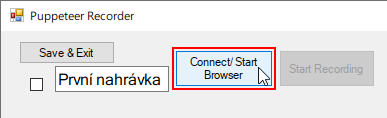
\includegraphics[width=0.7\textwidth]{connectToBrowser.png}
		\caption{Spouštění backendu a~Chromu}
	\end{figure}
	\newpage
	Měla by se nám otevřít nová instance Chromu s~jedním prázdným otevřeným oknem. UI by mělo povolit zakázané tlačítko "Start Recording" a~vypadat takto: 
	\begin{figure}[H]
		\centering
		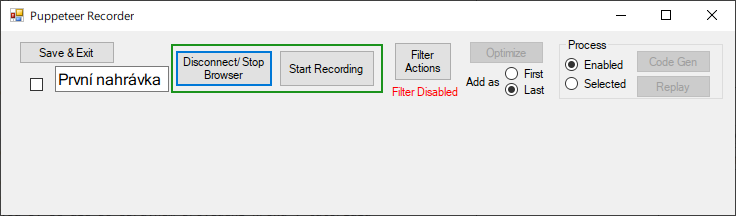
\includegraphics[width=1.0\textwidth]{emptyRecordingAfterConnection.png}
		\caption{Editační UI po spuštění backendu a~prohlížeče}
	\end{figure}
	Pokud UI tak nevypadá a~Chrome se neotevřel, objevila zpráva s~chybou, ta vždy popisuje konkrétní problém včetně kroků, které je nutné podniknou pro její odstranění, chyba by se ale po správném provedení kroků v~\refFullAddedText{subsub_sec:firstRun}{tutoriálu }{} objevit neměla.
	
	Stiskem tlačítka "Start Recording" spustíme nahrávání akcí provedených s~otevřenou instancí Chromu. Pro seznam podporovaných akcí odkážeme čtenáře do \fullNameref{sub_sec:functionalityComparison}.
	\begin{figure}[H]
		\centering
		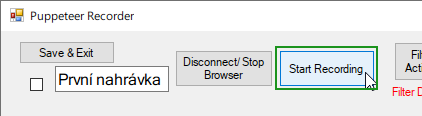
\includegraphics[width=0.76\textwidth]{startRecordingClick.png}
		\caption{Zapnutí nahrávání akcí}
	\end{figure}
	Nahrajme si libovolný počet akcí. Nahrání akce poznáme přidáním odpovídajícího řádku do UI.
	\begin{figure}[H]
		\centering
		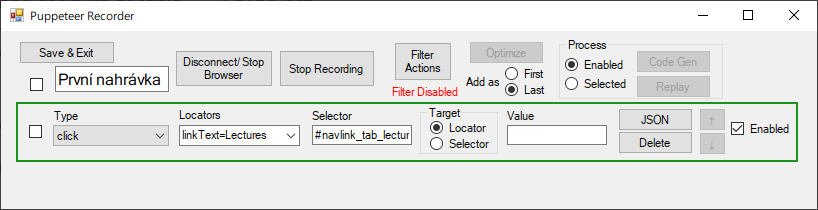
\includegraphics[width=1.0\textwidth, center]{oneActionRecorded.png}
		\caption{Nahrání první akce}
	\end{figure}
	Pro ukončení nahrávání akcí klikneme na tlačítko "Stop Recording".
	\nopagebreak
	\begin{figure}[H]
		\centering
		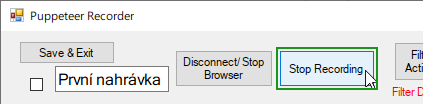
\includegraphics[width=0.76\textwidth, center]{stopRecordingClick.png}
		\caption{Vypnutí nahrávání akcí}
	\end{figure}
	Nyní nás již dělí jediný krok od generování kódu pro Puppeteer a~přehrávání akcí, tím krokem je optimalizace akcí. Při nahrávání akcí často nahrajeme spoustu akcí z~nichž značná část je pro přehrávání nepodstatná\footnote{Uvedeme příklad jednoduše popsatelné nepodstatné akce: Při vyplňování textového políčka se nahrají události "input", po vyplnění a~opuštění políčka se nahraje událost "change". Pro přehrávání nám stačí pouze událost "change". Optimalizace v~tomto případě odstraní všechny události "input". Uvědomme si však, že řešením není nahrávat pouze události "change" a~úplně ignorovat události "input". V~tomto případě by se mohlo stát, že uživatel vyplní textové políčko, neopustí ho, vypne nahrávání a~akce s~vyplněním políčka nebude nahrána.}. Pro smazání snadno popsatelných nadbytečných akcí je zde přítomno tlačítko "Optimize". Klikem na toto tlačítko nyní optimalizaci provedeme.
	\begin{figure}[H]
	\centering
	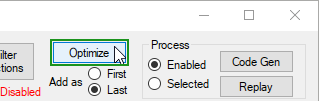
\includegraphics[width=0.57\textwidth, center]{optimizeClick.png}
	\caption{Optimalizace akcí}
	\end{figure}
	\newpage
	Aktuálně nám již nic nebrání vyzkoušet si vygenerovat kód a~přehrát akce. 
	\begin{figure}[H]
		\centering
		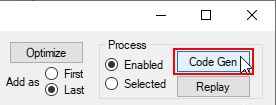
\includegraphics[width=0.50\textwidth]{codeGenButton.png}
	\end{figure}
	\vspace{-0.7cm}
	\begin{figure}[H]
		\centering
		\textdownarrow
	\end{figure}
	\vspace{-0.6cm}
	\begin{figure}[H]
		\centering
		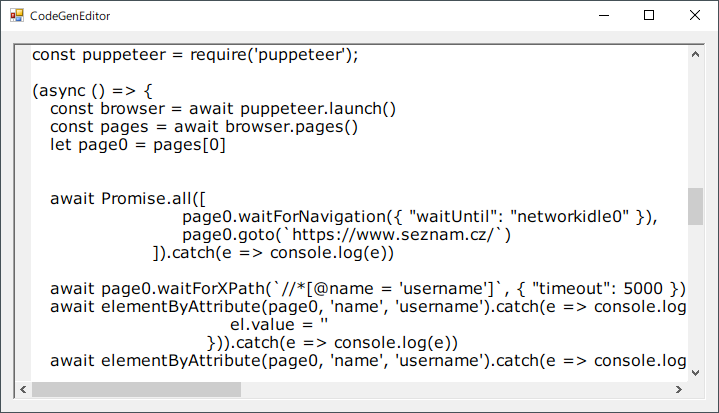
\includegraphics[width=1.0\textwidth]{codeGenEditor.png}
		\caption{Zobrazení kódu pro Puppeteer odpovídající nahraným akcím}
	\end{figure}
	Akce přehrajeme kliknutím na tlačítko "Replay". 
	\begin{figure}[H]
		\centering
		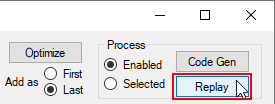
\includegraphics[width=0.50\textwidth]{replayButton.png}
		\caption{Zapnutí přehrávání akcí}
	\end{figure}
	Po kliku se nám zvýrazní právě přehrávaná akce. 
	\nopagebreak
	\begin{figure}[H]
		\centering
		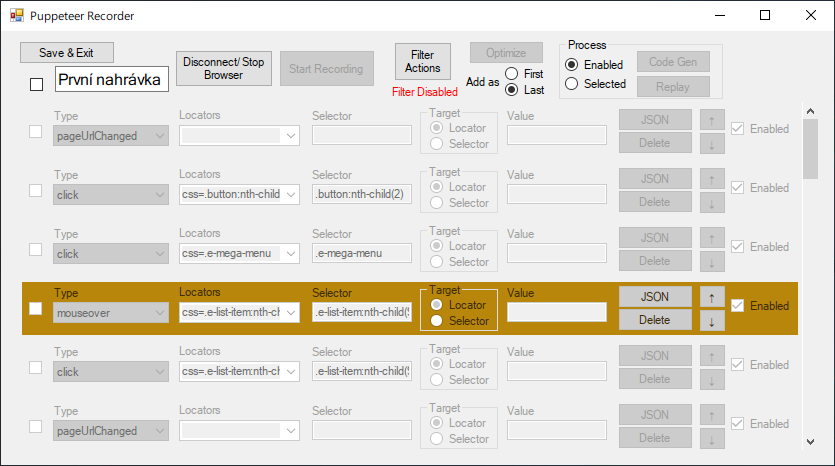
\includegraphics[width=1.0\textwidth]{replaying.png}
		\caption{Spuštění přehrávání akcí}
	\end{figure}
	Otevře se i~nové okno popisující stav probíhajícího přehrávání. Zde se zobrazí případné chyby\footnote{Chybami rozumíme neexistenci elementu a~existenci více elementů pro daný identifikátor.} při přehrávání akcí, probíhající přehrávání je možné tlačítkem "Stop Replaying" náhle ukončit. 
	\begin{figure}[H]
		\centering
		\includegraphics[width=1.0\textwidth]{replayView.png}
		\caption{Okno popisující stav spuštěného přehrávání}
	\end{figure}
	\newpage
	Při kliknutí na zprávu oznamující chybu se nám v~editačním UI zvýrazní akce, která chybu vyvolala.
	\begin{figure}[H]
		\centering
		\begin{subfigure}[t]{1.0\textwidth}
			\includegraphics[width=1.0\textwidth]{errorClick.png}
			\caption{}
			\label{subfig:errorClick}
		\end{subfigure}
	\end{figure}
	\vspace{-0.7cm}
	\begin{figure}[H]\ContinuedFloat
		\centering
		\textdownarrow
	\end{figure}
	\vspace{-0.6cm}
	\begin{figure}[H]\ContinuedFloat
		\centering
		\begin{subfigure}[t]{1.0\textwidth}
			\includegraphics[width=1.0\textwidth]{highlightedError.png}
%			\caption{}
		\end{subfigure}
		\caption{Zvýraznění akce, která vyvolala chybu}
	\end{figure}
	Po dokončení přehrávání se nám v~okně popisující přehrávání objeví zpráva "Replay Ended", ta je zvýrazněna zeleným rámečkem na \cref{subfig:errorClick}.
	
	Přesuneme se od přehrávání -- vraťme se nyní do hlavního spouštějícího okna frontendu. Okno popisující přehrávání zavřeme, odpojíme se od prohlížeče a~vypneme backend. 
	\begin{figure}[H]
		\centering
		\includegraphics[width=0.69\textwidth]{disconnectFromBrowser.png}
		\caption{Odpojení prohlížeče a~vypnutí backendu}
	\end{figure}
	\newpage
	Nakonec uložíme nahrávku a~vrátíme se do seznamu všech uložených nahrávek.
	\begin{figure}[H]
		\centering
		\begin{subfigure}[t]{1.0\textwidth}
			\centering
			\includegraphics[width=0.50\textwidth]{saveAndExit.png}
		\end{subfigure}
	\end{figure}
	\vspace{-0.7cm}
	\begin{figure}[H]\ContinuedFloat
		\centering
		\textdownarrow
	\end{figure}
	\vspace{-0.6cm}
	\begin{figure}[H]\ContinuedFloat
		\centering
		\begin{subfigure}[t]{1.0\textwidth}
			\centering
			\includegraphics[width=0.93\textwidth]{mainPage.png}
			%			\caption{}
		\end{subfigure}
		\caption{Uložení nahrávky a~návrat do seznamu všech uložených nahrávek}
	\end{figure}
	\subsubsection{Připojení ke vzdálenému Chromu}
	\label{subsub_sec:remoteChrome}
	Pro účely tohoto tutoriálu je nutné mít připravenou jednu nahrávku a~dva počítače. Předpokládejme následující schéma zapojení. 
	\begin{figure}[H]
		\centering
		\includegraphics[width=0.6\textwidth]{remoteConnectionSchema.pdf}
		\caption{Schéma zapojení počítačů}
	\end{figure}
	Na serveru spustíme Chrome s~parametrem \texttt{--remote-debugging-port=9222}, s~tímto parametrem běží ve Chromu CDP na portu 9222. Na CDP takto spuštěné instance Chromu je možné se připojit pouze z~localhost~\cite{devtoolsProtocol}, abychom CDP zpřístupnili vzdáleně, musíme přesměrovat nějaký jiný vzdáleně přístupný port na port 9222. Tohoto je možné docílit spuštěním následujícího příkazu na serveru~\cite{enableTrueRemoteDebuggingChrome}.
	\nopagebreak
	\begin{codefigure}[H]
		\renewcommand\baselinestretch{\codefigureSpacing}
		\begin{lstlisting}[style=MyHTML]
ssh -L 0.0.0.0:9223:localhost:9222 localhost -N
		\end{lstlisting}
		\caption{Přesměrování vzdáleně přístupného portu 9223 na port 9222}
	\end{codefigure}
	Nyní stačí nastavit ve frontendové části připojení ke Chromu na "Connect", zadat korektní IP adresu s~portem.
	\begin{figure}[H]
		\centering
		\begin{minipage}{0.45\textwidth}
			\begin{subfigure}[t]{1.0\textwidth}
				\includegraphics[width=1.0\textwidth]{browserConnectionChange.png}
			\end{subfigure}	
		\end{minipage}
		\hfill
		\textrightarrow
		\hfill
		\begin{minipage}{0.45\textwidth}
			\begin{subfigure}[t]{1.0\textwidth}
				\includegraphics[width=1.0\textwidth, right]{browserConnectFilled.png}
			\end{subfigure}	
		\end{minipage}
		\caption{Nastavení připojení na "Connect" s~vyplněním IP adresy a~portu}
	\end{figure}
	Můžeme si vyzkoušet přehrát připravenou nahrávku. Připojení ke Chromu a~spuštění backendu tlačítkem "Connect/Start Browser" nespustí novou instanci Chromu, ale připojí se k~již existující na serveru. Přehrávání nahrávky se odehraje na serveru.
	\subsubsection{Tlačítko JSON}
	\label{subsub_sec:jsonTutorial}
	Součástí každé nahrané akce je tlačítko "JSON". 
	\nopagebreak
	\begin{figure}[H]
		\centering
		\includegraphics[width=1.0\textwidth]{jsonButton.png}
		\caption{Tlačítko JSON jako součást každé akce}
		\label{fig:jsonButtonHighlight}
	\end{figure}
	Po kliku na toto tlačítko se zobrazí textová nezpracovaná data ve formátu JSON popisující nahranou akci.
	\begin{figure}[H]
		\centering
		\includegraphics[width=0.97\textwidth]{jsonEditor.png}
		\caption{Data ve formátu JSON popisující nahranou akci "pageUrlChanged"}
		\label{fig:jsonEditor}
	\end{figure}
	\Cref{fig:jsonEditor} popisuje podle parametru "type" událost "pageUrlChanged". Mezi další užitečné parametry patří "oldUrl" a~"newUrl", zřejmě z~jejich názvů: První parametr popisuje původní adresu URL, druhý pak novou adresu, která byla načtena. Ani jeden z~těchto parametrů nemá vlastní UI viz \cref{fig:jsonButtonHighlight}, a~proto jediná možnost nahlédnutí na~konkrétní hodnoty je přes data v~JSONu.
	
	\newpage
	Pokud bychom potřebovali nezpracovaná data v~JSONu měnit, např. chceme načíst jinou adresu URL, máme k~dispozici zaškrávací políčko s~popiskem "Modifications" (zvýrazněno zeleným rámečkem na \cref{fig:jsonEditor}), které při zaškrtnutí povolí modifikace. Dovolujeme si ale upozornit, že takto provedené modifikace jsou prováděny na vlastní nebezpečí a~při neplatné modifikaci je možné akci i~znefunkčnit.
	\begin{figure}[H]
		\centering
		\includegraphics[width=0.97\textwidth]{jsonModificationInProgress.png}
		\caption{Modifikace nezpracovaných dat v~JSONu}
	\end{figure}
	\subsubsection{Výběr akcí ke zpracování}
	Některé nahrávky mohou obsahovat spousty akcí, ne vždy budeme chtít všechny přehrát. Dokonce můžou nastat situace, kdy budeme chtít výhradně pro debuggovací účely přehrát jednu jedinou akci -- totéž platí kromě přehrávání i~pro generování kódu. V~tomto tutoriálu si ukážeme jak na to.
	
	Přesuňme se do editačního UI libovolné nahrávky. Jak již bylo naznačeno v~úvodním odstavci, výběr akcí je možný pro přehrávání i~pro generování kódu. 
	\begin{figure}[H]
		\centering
		\includegraphics[width=0.49\textwidth]{actionsToProcess.png}
		\caption{Přepínače pro výběr akcí ke zpracování}
		\label{fig:processType}
	\end{figure}	
	\Cref{fig:processType} nám ukazuje, že je možné zpracovat buďto akce povolené ("Enabled") nebo akce vybrané ("Selected").\newpage Na následujícím obrázku jsou odpovídající zaškrtávací políčka pro výběr a~povolení akcí zvýrazněna stejnou barvou jako na \cref{fig:processType}.
	\begin{figure}[H]
		\centering
		\begin{subfigure}[t]{0.48\textwidth}
			\includegraphics[width=1.0\textwidth, left]{selectActions.png}
			\caption{Výběr akce}
		\end{subfigure}	
		\hfill
		\begin{subfigure}[t]{0.46\textwidth}
			\includegraphics[width=1.0\textwidth, right]{enableActions.png}
			\caption{Povolení akce}
		\end{subfigure}	
		\caption{Zaškrtávací políčka pro výběr a~povolení akcí}
	\end{figure}
	Na závěr tohoto tutoriálu přikládáme ukázku vygenerování kódu jedné akce typu "pageUrlChanged". 
	\begin{figure}[H]
		\begin{minipage}{0.47\textwidth}
			\begin{subfigure}[t]{1.0\textwidth}
				\includegraphics[width=1.0\textwidth]{actionSelected.png}
			\end{subfigure}
		\end{minipage}
		\hfill
		\textrightarrow
		\hfill
		\begin{minipage}{0.47\textwidth}
			\begin{subfigure}[t]{1.0\textwidth}
				\includegraphics[width=1.0\textwidth, right]{codeGenSelected.png}
			\end{subfigure}
		\end{minipage}
	\end{figure}
	\vspace{-1.0cm}
	\begin{figure}[H]\ContinuedFloat
		\hfill
		\begin{minipage}{0.205\textwidth}
			\begin{turn}{45}
				\textleftarrow
			\end{turn}
		\end{minipage}
	\end{figure}
	\begin{figure}[H]\ContinuedFloat
		\centering
		\includegraphics[width=1.0\textwidth]{pageUrlChangedCodeGen.png}
		\caption{Vygenerování kódu jedné akce typu "pageUrlChanged"}
	\end{figure}
	\subsubsection{Filtr akcí}
	V~horní části editačního UI je ještě jedno tlačíko, na které jsme se zatím v~žádném tutoriálu nepodívali. Tlačítko má popisek "Filter Actions", který nám napodívá, že jedná se o~filtr. V~našem případě umožňuje dočasně skrýt akce dle různých kritérií\footnote{Kritéria, která můžeme použít pro filtrování i~současně:
		\begin{itemize}[noitemsep, topsep=1pt]
			\item[--] typ události (pageUrlChanged, click, scroll, ...)
			\item[--] typ identifikátoru (lokátor, selektor)
			\item[--] stav akce (povolená, vybraná)
		\end{itemize} 
	}.

	Přesunňme se do existující nahrávky a~klikněme na tlačítko pro filtraci.
	\begin{figure}[H]
		\centering
		\begin{subfigure}[t]{1.0\textwidth}
			\centering
			\includegraphics[width=1.0\textwidth]{filterActionsClick.png}
			\caption{Klik na tlačítko "Filter Actions"}
			\label{subfig:editFilterActions}
		\end{subfigure}
	\end{figure}
	\vspace{-0.7cm}
	\begin{figure}[H]\ContinuedFloat
		\centering
		\textdownarrow
	\end{figure}
	\vspace{-0.6cm}
	\begin{figure}[H]\ContinuedFloat
		\centering
		\begin{subfigure}[t]{1.0\textwidth}
			\centering
			\includegraphics[width=0.42\textwidth]{filterFormJustRun.png}
			\caption{Okno pro aplikaci filtrů}
			\label{subfig:filterForm}
		\end{subfigure}
		\caption{Otevření okna pro aplikaci filtrů}
	\end{figure}
	Všimněme si, že na \cref{subfig:editFilterActions} je pod stisknutým tlačítkem napsáno "Filter Disabled", což značí neaktivitu filtru. Dále se podívejme, že na stejném obrázku se mezi čtyřmi nahranými akcemi nachází nejprve dvakrát za sebou akce typu "pageUrlChanged" a~potom dvakrát za sebou akce typu "click". Filtr využijeme tak, že skryjeme poslední dvě akce.
	
	Pro použití filtru nejprve musíme aktivovat filtr odpovídající kategorie. To se provádí zaškrtnutím políčka s~popiskem "Enabled". Políčko pro aktivaci filtru dle typu akce je zvýrazněno červeným rámečkem na \cref{subfig:filterForm}.
	
	Tuto aktivaci filtru provedeme, poté zaškrtneme políčko s~popiskem "Browser App Events" a~"Viewport Events". První zmíněné políčko povolí filtrování akcí pocházejících z~okna prohlížeče, druhé povolí fitrování akcí z~viewportu. 
	\begin{figure}[H]
		\centering
		\begin{minipage}{0.47\textwidth}
			\begin{subfigure}[t]{1.0\textwidth}
				\includegraphics[width=1.0\textwidth]{filterForm2.png}
				\caption{Aktivace filtru dle typu akce}
			\end{subfigure}	
		\end{minipage}
		\hfill
		\textrightarrow
		\hfill
		\begin{minipage}{0.47\textwidth}
			\begin{subfigure}[t]{1.0\textwidth}
				\includegraphics[width=1.0\textwidth, right]{filterForm3.png}
				\caption{Povolení filtrování akcí pocházejících z~okna prohlížeče i~z~viewportu}
				\label{subfig:filterEnableForAllTypes}
			\end{subfigure}	
		\end{minipage}
		\caption{Aktivace filtru pro akce pocházející z~okna prohlížeče a~viewportu}
	\end{figure}
	Zaškrnutá políčka, která jsou obsažena v~červeném rámečku na \cref{subfig:filterEnableForAllTypes} značí typy akcí, které budou zobrazeny v~editačním UI.\newpage Pro skrytí posledních dvou akcí typu "click" stačí pouze odškrtnout políčko s~popiskem "Click".
	\begin{figure}[H]
		\centering
		\begin{subfigure}[t]{1.0\textwidth}
			\centering
			\includegraphics[width=0.51\textwidth]{filterForm4.png}
			\caption{Odškrtnutí políčka s~popiskem "Click"}
		\end{subfigure}
	\end{figure}
	\vspace{-0.7cm}
	\begin{figure}[H]\ContinuedFloat
		\centering
		\textdownarrow
	\end{figure}
	\vspace{-0.6cm}
	\begin{figure}[H]\ContinuedFloat
		\centering
		\begin{subfigure}[t]{1.0\textwidth}
			\centering
			\includegraphics[width=1.0\textwidth]{filtered.png}
			\caption{Editační UI se zapnutým filtrem}
			\label{subfig:editUiFiltered}
		\end{subfigure}
		\caption{Skrytí dvou akcí typu "click" pomocí filtru}
	\end{figure}
	Všimňeme si, že na \cref{subfig:editUiFiltered} se nyní pod tlačítkem s~popiskem "Filter Actions" nachází text zelené barvy "Filter Enabled" informující o~zapnutí filtru.
	\subsubsection{Změna identifikátoru akce}
	%jak upravit selektor, vyber z lokatoru, zminit jak si pridat vlastni lokator
	Akce pocházející z~viewportu prohlížeče jsou vždy vykonány nad elementem, který je potřeba identifikovat. K~tomu nám slouží vhodný selektor nebo lokátor. V~tomto tutoriálu si ukážeme jak pracovat se selektory a~lokátory.
	
	Přesuneme se opět do editačního UI existující nahrávky. Barvy rámečků na~následujícím obrázku zobrazují vztahy mezi přepínači a~políčky.
	\nopagebreak
	\begin{figure}[H]
		\centering
		\includegraphics[width=1.0\textwidth]{identifiers2.png}
		\caption{Vztahy mezi přepínači a~políčky}
		\label{fig:identifierRelationship}
	\end{figure}
	Na \cref{fig:identifierRelationship} je vybrán přepínač (3), jako identifikátor se bude brát v~potaz pouze hodnota selektoru (2).
	
	Pokud bychom naopak chtěli použít lokátor jako identifikátor, stačí aby byl vybrán přepínač (4). V~tomto případě se bude ignorovat hodnota (2) a~použije se vybraný lokátor (1), povšimněme si, že se jedná o~combo box -- obvykle totiž existuje více různých lokátorů identifikujících element.
	\begin{figure}[H]
		\centering
		\includegraphics[width=1.0\textwidth]{allLocators.png}
		\caption{Seznam dostupných lokátorů pro konkrétní akci typu "click"}
	\end{figure}
	\newpage
	Pokud bychom chtěli použít vlastní lokátor, který není v~seznamu mezi dostupnými, můžeme přepsat hodnotu combo boxu na libovolný vlastní lokátor.
	\nopagebreak
	\begin{figure}[H]
		\centering
		\includegraphics[width=0.69\textwidth]{customLocator.png}
		\caption{Vlastní lokátor}
	\end{figure}
	Seznam všech různých typů lokátorů je uveden
v~\hyperref[tab:locatorsList]{\cref{tab:locatorsList} na straně \pageref{tab:locatorsList}}.
	
	Čtenáře, který pečlivě četl \refFullAddedText{subsub_sec:firstRun}{tutoriál }{} jistě napadne, že další způsob přidání i~většího množství vlastních lokátorů je pomocí tlačítka "JSON". 
	
	Data ve formátu JSON popisující akci typu "click" vypadají takto:
	\begin{figure}[H]
		\centering
		\includegraphics[width=1.0\textwidth]{clickActionJson.png}
		\caption{Data ve formátu JSON akce typu "click"}
	\end{figure}
	Po povolení modifikací můžeme přidat další lokátory.
	\nopagebreak
	\begin{figure}[H]
		\centering
		\includegraphics[width=1.0\textwidth]{customLocatorJSON.png}
		\caption{Přidání nového lokátoru}
	\end{figure}
	\newpage
	\subsection{Detaily implementace}
	\label{sub_sec:programmerDocs}
	V~této podsekci se budeme zabývat podrobněji backendem a~frontendem. Nebudeme se zde zabývat návrhem celého řešení, ten je popsán v~\fullNameref{sub_sec:design}, kam odkážeme případné zájemce.
	
	Součástí nebudou detailní rozbory zdrojových kódu a~dalších jiných technických aspektů. Tato sekce slouží pouze jako rozcestník, zájemci po jejím přečtení budou schopni nalézt zdrojový soubor s~hledanou funkcionalitou. Pro hladší pochopení jsou zdrojové soubory komentovány vždy na úrovni tříd a~většiny metod, zejména pak těch netriviálních.
	%nazev souboru
	%obsazene tridy
	%letmy popis
	%nektere obsazene metody
	%okno formulare
	\subsubsection{Backend}
	\label{subsub_sec:backendProgrammersDocs}
	Backendová část se nachází v~adresáři \texttt{Backend\textbackslash}. Názvy podsekcí spadající pod tuto sekci odpovídají zdrojovým souborům, a~proto předpokládáme, že se nacházíme v~cestě \texttt{Backend\textbackslash src}. Zdrojové soubory jsou uvedeny v~abecedním pořadí počínaje soubory nacházejícími se v~podadresářích.
	%Pro backendovou část vytvoříme primárně rozcestník, který bude sloužit pro rychlou orientaci ve zdrojových souborech.
	\subsubsubsection{JsExtensions\textbackslash ArrayExtensions.js}
	Jednoduché metody rozšiřující \texttt{Array} objekt JavaScriptu.
	\paragraph{Třídy}
	\xmark
	\paragraph{Vybrané metody}
	\begin{lstlisting}[style=JSProgrammersDocs]
Object.assign(Array.prototype, {
	removeAt(index) { this.splice(index, 1) }
})
	\end{lstlisting}
	
	\subsubsubsection{JsExtensions\textbackslash ObjectExtensions.js}
	Jednoduché metody rozšiřující \texttt{Object} objekt JavaScriptu.
	\paragraph{Třídy}
	\xmark
	\paragraph{Vybrané metody}
	\begin{lstlisting}[style=JSProgrammersDocs]
Object.assign(Object.prototype, {
	empty() { return Object.keys(this).length === 0 }
})
	\end{lstlisting}
	
	\subsubsubsection{JsExtensions\textbackslash StringExtensions.js}
	Jednoduché metody rozšiřující \texttt{String} objekt JavaScriptu.
	\paragraph{Třídy}
	\xmark
	\paragraph{Vybrané metody}
	\begin{lstlisting}[style=JSProgrammersDocs]
Object.assign(String.prototype, {
	containsNumber() { return /^-?\d+$/.test(this) }
})
	\end{lstlisting}
	\subsubsubsection{PuppeteerExtensions\textbackslash BrowserExtensions.js}
	\label{docs:browserExtensions}
	Několik metod rozšiřujících standardní funkcionalitu \texttt{Browser} objektu Puppeteeru. Součástí je i~kód redefinující zejména událost "tabcreated". Toho je využíváno pro inicializaci rozšíření nově otevřených stránek viz. \ref{docs:pageExtensions}.
	\paragraph{Třídy}
	\xmark
	\paragraph{Vybrané metody}
	\begin{methods}
	\lstinline[style=JSProgrammersDocs]|async function addBrowserExtensions(browser)| přidá všechna rozšíření do prohlížeče \lstinline|browser|.
	
	\lstinline[style=JSProgrammersDocs]|async function _getActivePage(browser, timeoutMs)| vrátí aktuálně aktivní tab patřící prohlížeči \lstinline|browser|. Tato metoda nepoběží déle než \lstinline|timeoutMs|.
	\end{methods}
	\subsubsubsection{PuppeteerExtensions\textbackslash PageExtensions.js}
	\label{docs:pageExtensions}
	Několik metod rozšiřujících standardní funkcionalitu \texttt{Page} objektu Puppeteeru.
	\paragraph{Třídy}
	\xmark
	\paragraph{Vybrané metody}
	\begin{methods}
		\lstinline[style=JSProgrammersDocs]|async function addPageExtensions(page)| přidá všechna rozšíření do stránky \lstinline|page|.
		
		\lstinline[style=JSProgrammersDocs]|async function _cdpExecute(page, cmds)| odešle požadavek stránce \lstinline|page| na volání CDP funkce dané \lstinline|cmds|.
		
		\lstinline[style=JSProgrammersDocs]|function _clearExposedFunctionsBindings(page)| odstraní všechny funkce, které byly dříve zveřejněny na stránce \lstinline|page|.
		
		\lstinline[style=JSProgrammersDocs]|function _removeExposedFunctionByName(page, fName)| odstraní funkci, která byla dříve zveřejněna na stránce \lstinline|page| podle jména \lstinline|fName|.
	\end{methods}
	\subsubsubsection{selenium-ide-src\textbackslash LocatorPkg.js}
	\label{docs:locatorsFile}
	Funkcionalita lokátorů pochází ze zdrojového kódu projektu Selenium IDE~\cite{seleniumIdeGithub}. Na~tento kód se vztahuje licence Apache 2.0 v~souladu se~kterou je kód využit.
	\paragraph{Třídy}
	Jedná se sice o~velké množství kódu, většina ale pochází z~doby, kdy JavaScript neobsahoval klíčové slovo \texttt{class}. Pokud budeme brát v~potaz objekty vytvořené přes funkce, jak to bývalo tradiční v~JavaScriptu, pak do tohoto seznamu můžeme zahrnout \texttt{LocatorBuilders}.
	\paragraph{Vybrané metody}
	\begin{methods}
		\lstinline[style=JSProgrammersDocs]|LocatorBuilders.prototype.buildAll = function(el)| vrátí seznam lokátorů identifikující \lstinline|el|, což je objekt typu \lstinline|Element| odpovídající nějakému existujícímu elementu na stránce.
	\end{methods}
	\subsubsubsection{WindowFunctions\textbackslash LocatorTransformation.js}
	\label{docs:locatorTransformation}
	Metody pro transformaci nezpracovaných lokátorů získaných pomocí funkce \texttt{buildAll} viz \ref{docs:locatorsFile}.
	\paragraph{Třídy}
	\xmark
	\paragraph{Vybrané metody}
	\begin{methods}
	\lstinline[style=JSProgrammersDocs]|function transformLocators(locators)| vyextrahuje CSS lokátor z~pole\newline\lstinline|locators|, vrátí dvě hodnoty: pole zbylých lokátorů a~CSS lokátor.
	\end{methods}
	\subsubsubsection{BrowserConnectionLayer.js}
	\label{docs:browserConnectionLayer}
	Abstrakční vrstva pro inicializaci Puppeteeru umožňující propojení s~prohlížečem.
	\paragraph{Třídy}
	\texttt{BrowserConnectionLayer}
	\paragraph{Vybrané metody}
	\begin{methods}
		\lstinline[style=JSProgrammersDocs]|async cdpExecuteAllPages(cmds)| provede okamžitě volání CDP funkcí daných parametrem \lstinline|cmds| na všech otevřených stránkách.
		
		\lstinline[style=JSProgrammersDocs]|async initializeBrowser()| přidá do objektu prohlížeče rozšíření z~\ref{docs:browserExtensions}.
		
		\lstinline[style=JSProgrammersDocs]|async launch(options)| připojí Puppeteer k~prohlížeči voláním\newline \lstinline|puppeteer.launch(options)|. Následně přidá do objektu prohlížeče rozšíření z~\ref{docs:browserExtensions}.
		
		\lstinline[style=JSProgrammersDocs]|setNewPageCDPExecute(cmds)| nastaví volání CDP funkcí daných parametrem\linebreak\lstinline|cmds| pro každý nově otevřený tab.
	\end{methods}
	\subsubsubsection{CodeGenerator.js}
	Logika generování kódu pro Puppeteer.
	\paragraph{Třídy}
	\texttt{CodeGenerator}
	\paragraph{Vybrané metody}
	\begin{methods}
		\lstinline|codeGen(actions)| vygeneruje kód akce/akcí v~proměnné \lstinline|actions|.
		
		\lstinline|_addPermissionToCurrPage(permission)| přidá požadavek na oprávnění\newline\lstinline|permission| pro aktuální URL aktivní stránky.
		
		\lstinline|_catchAndLogErrors(code)| vygeneruje kód pro logování a~zachytávání výjimek podle hodnot v~\lstinline|this._options.catchErrors| a~\lstinline|this._options.logErrors|.
		
		\lstinline|_codeGenBlock(actions, i)| generuje blok kódu z~\lstinline|actions[i]|. Vygenerovaný blok se skládá ze tří částí: prologue, main a~epilogue.
		
		\lstinline|_genDOMEventFromIdentifier(id, eventName)| generuje volání \lstinline|Page.evaluate| nebo \lstinline|ElementHandle.evaluate| obsahující událost DOM. Typ volání a~element aktivující událost jsou určeny na základě identifikátoru \lstinline|id|, název události je dán parametrem \lstinline|eventName|.
		
		\lstinline|_genGivePermissions()| vygeneruje kód pro získání oprávnění na základě předchozích volání metody \lstinline|_addPermissionToCurrPage|.
		
		\lstinline|_genWaitForIdentifier(id)| vygeneruje volání \lstinline|Page.waitForXPath| nebo\newline\lstinline|Page.waitForSelector| dle typu identifikátoru \lstinline|id|.
		
		\lstinline|_genWaitForNavCall()| vygeneruje volání \lstinline|Page.waitForNavigation|.
		
		\lstinline|_identifier(action)| vrátí identifikátor akce \lstinline|action|, který byl vybrán ve frontendu.
		
		\lstinline|_plainCode(codeBlocks)| převede bloky kódu vygenerované metodou\newline\lstinline|_codeGenBlock| do kódu pro Puppeteer.
		
	%	\enlargethispage{\baselineskip}
		Mnoho dalších metod generujících volání:\newline \lstinline|_browserFuncCall|, \lstinline|_genExecRawCodeInsidePage|, \lstinline|_genIdentifierFuncCall|,\linebreak\lstinline|_pageFuncCall|, ... Více informací o~těchto a~dalších metodách je uvedeno v~komentářích ve zdrojovém souboru.
	\end{methods}
	\subsubsubsection{main.js}
	Spouštějící soubor backendové části, čeká na zprávy z~backendu, které předá ke~zpracování.
	\paragraph{Třídy}
	\xmark
	\paragraph{Vybrané metody}
	\begin{methods}
		\lstinline[style=JSProgrammersDocs]|function processCmd(cmd)| zpracuje příkaz \lstinline|cmd| pocházející z~frontendu.
	\end{methods}
	
	\subsubsubsection{Optimizer.js}
	\label{docs:optimizer}
	\paragraph{Třídy}
	\texttt{Optimizer}
	\paragraph{Vybrané metody}
	\begin{methods}
		\lstinline[style=JSProgrammersDocs]|optimizeRecordings(rec)| smaže nevýznamné, nadbytečné akce pole \lstinline|rec|, navrátí nové pole bez těchto akcí.
	\end{methods}
	\subsubsubsection{Recorder.js}
	Logika nahrávání akcí pocházejících z~okna prohlížeče i~viewportu.
	\paragraph{Třídy}
	\texttt{Recorder}, dědí od třídy \texttt{BrowserConnectionLayer} viz \ref{docs:browserConnectionLayer}.
	\paragraph{Vybrané metody}
	\begin{methods}
		\lstinline[style=JSProgrammersDocs]|async optimize()| provede optimalizaci nahraných akcí viz \ref{docs:optimizer}.
		
		\lstinline[style=JSProgrammersDocs]|setEventsToRecord(events)| nastaví události k~nahrávání podle \lstinline|events|.
		
		\lstinline[style=JSProgrammersDocs]|async start(cleanStart = true)| spustí nahrávání akcí, \lstinline|cleanStart| udává, jestli máme vyčistit pole již nahraných akcí.
		
		\lstinline[style=JSProgrammersDocs]|async stop()| zastaví probíhající nahrávání akcí.
		
		\lstinline[style=JSProgrammersDocs]|async _connectViewportEvents(page)| spustí na stránce \lstinline|page| kód pro zachytávání a~předávání akcí zpátky do backendové aplikace.
	\end{methods}
	
	\subsubsubsection{WindowFunctionsUtils.js}
	Metody umožňující zveřejnit obsah zdrojového souboru do proměnné \texttt{window} okna prohlížeče.
	\paragraph{Třídy}
	\xmark
	\paragraph{Vybrané metody}
	\begin{methods}
		\lstinline[style=JSProgrammersDocs]|async function addWindowFunctionsToPage(page)| přidá do proměnné \lstinline|window| stránky \lstinline|page| obsah souborů \ref{docs:locatorsFile} a~\ref{docs:locatorTransformation}.
	\end{methods}
	
	\subsubsubsection{ZeroMQUtils.js}
	Několik metod usnadňujících práci se~ZeroMQ.js.
	\paragraph{Třídy}
	\xmark
	\paragraph{Vybrané metody}
	\begin{lstlisting}[style=JSProgrammersDocs]
async function receiveMsg(sock) {
	return (await sock.receive()).toString('utf-8')
}
	\end{lstlisting}
	\newpage
	\subsubsection{Frontend}
	Visual Studio projekt frontendové části se nachází v~adresáři \texttt{Frontend\textbackslash}. Zdrojový kód pak v~adresáři \texttt{Frontend\textbackslash Frontend}, který považujeme nyní za aktuální cestu. Stejně jako v~předchozím \fullNameref{subsub_sec:backendProgrammersDocs}, i~zde názvy podsekcí odpovídají názvům zdrojových souborů, které jsou uvedeny v~abecedním pořadí.
	
	Upřesníme navíc ještě, že všechny formuláře se nachází v~adresáři \texttt{Forms\textbackslash} a~uživatelské komponenty (user control) využité ve formulářích pak v~\texttt{UserControls\textbackslash}.
	%Zde uvedeme strukturu a~význam celků frontendové části, oproti backendu tu navíc rozvedeme i~formuláře.
	\subsubsubsection{Forms\textbackslash CodeGenEditor.cs}
	\label{docs:codeGenEditor}
	Textový editor zobrazující vygenerovaný kód pro Puppeteer. Použitý textový editor je komponenta \texttt{ScintillaNET.Scintilla} projektu ScintillaNET~\cite{scintillaGithub} dostupného pod MIT licencí v~souladu se~kterou je komponenta využita. 
%	\paragraph{Formulář}
	\begin{figure}[H]
		\centering		\includegraphics[width=1.0\textwidth]{codeGenEditorDesc.png}
		\captionsetup{justification=centering}
		\caption[Formulář \texttt{CodeGenEditor} s~komponentou\newline \texttt{ScintillaNET.Scintilla}]{Formulář \texttt{CodeGenEditor} s~komponentou \texttt{ScintillaNET.Scintilla}}
	\end{figure}
	\paragraph{Třídy}
	\texttt{CodeGenEditor : Form}
	\paragraph{Vybrané metody}
	\lstinline[style=MyCSharpDocs]|public void SetEditorText(string txt)| nastaví textový řetězec \lstinline|txt| jako obsah textového editoru.
	\subsubsubsection{Forms\textbackslash CodeGenSettingsForm.cs}
	Nastavení parametrů pro generování kódu.
	\nopagebreak
%	\paragraph{Formulář}
%	\enlargethispage{\baselineskip}
	\begin{figure}[H]
		\centering
		\includegraphics[width=0.59\textwidth]{codeGeneratorSettingsForm.png}
		\caption{Formulář \texttt{CodeGenSettingsForm} s~komponentou \texttt{PropertyGrid}}
	\end{figure}
	\paragraph{Třídy}
	\texttt{CodeGenSettingsForm : Form}
	\paragraph{Vybrané metody}
	\begin{methods}
\lstinline[style=MyCSharpDocs]|public void BindCodeGeneratorOptions(CodeGenOptions c)| nastaví parametr~\lstinline|c| do komponenty property grid jako objekt k~úpravě.

\lstinline[style=MyCSharpDocs]|public CodeGenOptions ExportCodeGeneratorOptions()| vrátí objekt nastavený dle hodnot v~property gridu.
	\end{methods}
	\newpage
	\subsubsubsection{Forms\textbackslash FilterForm.cs}
	\label{docs:filterForm}
	Nastavení filtru.
	\nopagebreak
%	\paragraph{Formulář}
	\begin{figure}[H]
		\centering
		\includegraphics[width=0.51\textwidth]{filtrFormDocs.png}
		\caption{Formulář \texttt{FilterForm}}
	\end{figure}
	\paragraph{Třídy}
	\texttt{FilterForm : Form}
	\paragraph{Vybrané metody}
	\begin{methods}
		\lstinline[style=MyCSharpDocs]|public Filter ExportFilter()| vrátí objekt odpovídající aktuálnímu formuláři.
		
		\lstinline[style=MyCSharpDocs]|public void SetFilter(Filter f)| nastaví UI formuláře podle parametru \lstinline|f|.
	\end{methods}
	\newpage
	\subsubsubsection{Forms\textbackslash JsonEditor.cs}
	\label{docs:jsonEditor}
	Textový prohlížeč a~editor nezpracovaného JSONu odpovídající akci. Použitý textový editor je komponenta \texttt{ScintillaNET.Scintilla} projektu ScintillaNET~\cite{scintillaGithub} dostupného pod MIT licencí v~souladu se~kterou je komponenta využita. 
%	\paragraph{Formulář}
	\begin{figure}[H]
		\centering
		\includegraphics[width=0.97\textwidth]{jsonEditorDocs.png}
		\captionsetup{justification=centering}
		\caption[Formulář \texttt{JSONEditor} s~komponentou\newline\texttt{ScintillaNET.Scintilla}]{Formulář \texttt{JSONEditor} s~komponentou \texttt{ScintillaNET.Scintilla}}
	\end{figure}
	\paragraph{Třídy}
	\texttt{JsonEditor : Form}
	\paragraph{Vybrané metody}
	\begin{methods}
		\lstinline[style=MyCSharpDocs]|public string GetEditorText()| vrátí obsah textového editoru.
		
		\lstinline[style=MyCSharpDocs]|public void SetEditorText(string txt)| nastaví textový řetězec \lstinline|txt| jako obsah textového editoru. Hodnota vlastnosti \lstinline|ReadOnly| textového editoru zůstane zachována.
	\end{methods}
	\newpage
	\subsubsubsection{Forms\textbackslash MainForm.cs}
	\label{docs:mainForm}
	Hlavní spouštějící formulář frontendu, nachází se v~jednou ze dvou stavů~--~po spuštění je vždy ve stavu \texttt{AppMode.List}, kdy zobrazuje náhledy všech uložených nahrávek. Při vytvoření nové nahrávky nebo editaci existující se stav přepne do \texttt{AppMode.Edit}. Tyto dva stavy zobrazuje následující obrázek:
	\begin{figure}[H]
		\centering
		\begin{subfigure}[t]{1.0\textwidth}
			\includegraphics*[width=1.0\textwidth]{mainListState.png}
			\caption{\texttt{AppMode.List}}
		\end{subfigure}
	\end{figure}
	\begin{figure}[H]\ContinuedFloat
		\begin{subfigure}[t]{1.0\textwidth}
			\includegraphics*[width=1.0\textwidth]{mainEditState.png}
			\caption{\texttt{AppMode.Edit}}
			\label{fig:appModeEdit}
		\end{subfigure}
	\caption{Stavy \texttt{AppMode.List} a~\texttt{AppMode.Edit} formuláře \texttt{MainForm}}
	\end{figure}
	\paragraph{Třidy}
	\texttt{MainForm : Form}
	\paragraph{Vybrané metody}
	\begin{methods}
		\enlargethispage{\baselineskip}
		\lstinline[style=MyCSharpDocs]|private void MainForm_Load(object sender, EventArgs e)| spuštěna při načtení formuláře, načte uložené náhledy nahrávek a~zkontroluje existenci interpreteru Node.js.
		
		\lstinline[style=MyCSharpDocs]|protected override bool ProcessCmdKey(ref Message msg, Keys keyData)|\newline přetížení definující klávesovou zkratku Shift+Delete při editaci nahrávky. Tato zkratka odstraní akci s~vlastností \lstinline|Focus = true|.
		
		\lstinline[style=MyCSharpDocs]|public void SwitchToEditMode(Thumbnail t)| přepne formulář do stavu\linebreak\lstinline|AppMode.Edit| zobrazeném na \cref{fig:appModeEdit}. Parametr \lstinline|t| je náhled nahrávky, která je editována. V~případě, že \lstinline|t| není náhled nově vytvořené nahrávky, dříve uložené nahrané akce jsou načteny do formuláře.
		
		Další metody zpracovávající události UI:\newline \lstinline|addNewRecordingButton_Click|, \lstinline|MainForm_FormClosing|,\newline \lstinline|recorderToolStripMenuItem_Click|, ...
		
		A~metody upravující UI:\newline\lstinline|LoadThumbnailsUi|, \lstinline|NodeInterpterNotWorking|, \lstinline|PerformSettingsChecks|, \newline\lstinline|SetEditUiVisiblity|, \lstinline|SwitchToEditMode|, \lstinline|UiChange| ...
		
		Více informací o~všech těchto dalších metodách je uvedeno v~komentářích ve zdrojovém souboru.
	\end{methods}
	\subsubsubsection{Forms\textbackslash NodeJsConfig.cs}
	Nastavení cesty k~backendu a~interpreteru Node.js.
	\nopagebreak
%	\paragraph{Formulář}
	\begin{figure}[H]
		\centering
		\includegraphics[width=0.51\textwidth]{nodejsSettingsDocs.png}
		\caption{Formulář \texttt{NodeJsConfig}}
	\end{figure}
	\paragraph{Třidy}
	\texttt{NodeJsConfig : Form}
	\paragraph{Vybrané metody}
	\begin{methods}
		\lstinline[style=MyCSharpDocs]|public void BindNodeJsOptions(NodeJsOptions n)| nastaví UI formuláře podle parametru \lstinline|n|.
		
		\lstinline[style=MyCSharpDocs]|public NodeJsOptions ExportNodeJsOptions()| vrátí objekt odpovídající aktuálnímu formuláři.
	\end{methods}
	
	\subsubsubsection{Forms\textbackslash PlayerForm.cs}
	\label{docs:playerForm}
	Nastavení parametrů pro přehrávání akcí.
%	\paragraph{Formulář}
	\begin{figure}[H]
		\centering
		\includegraphics[width=0.52\textwidth]{playerFormDocs.png}
		\caption{Formulář \texttt{PlayerForm} s~komponentou \texttt{PropertyGrid}}
	\end{figure}
	\paragraph{Třidy}
	\texttt{PlayerForm : Form}
	\paragraph{Vybrané metody}
	\begin{methods}
		\lstinline[style=MyCSharpDocs]|public void BindNodeJsOptions(NodeJsOptions n)| nastaví parametr~\lstinline|n| do komponenty property grid jako objekt k~úpravě.
		
		\lstinline[style=MyCSharpDocs]|public NodeJsOptions ExportNodeJsOptions()| vrátí objekt nastavený dle hodnot v~property gridu.
	\end{methods}
	
	\subsubsubsection{Forms\textbackslash RecorderSettingsForm.cs}
	\label{docs:recorderSettings}
	Nastavení nahrávání a~prohlížeče.
%	\paragraph{Formulář}
	\nopagebreak
	\begin{figure}[H]
		\centering
		\includegraphics[width=0.90\textwidth]{recorderSettingsDocs.png}
		\captionsetup{justification=centering}
		\caption[Formulář \texttt{RecorderSettingsForm} s~uživatelskou komponentou\newline\texttt{PuppeteerOptionsUserControl}]{Formulář \texttt{RecorderSettingsForm} s~uživatelskou komponentou \texttt{PuppeteerOptionsUserControl}}
	\end{figure}
	\paragraph{Třidy}
	\texttt{RecorderSettingsForm : Form}
	\paragraph{Vybrané metody}
	\begin{methods}
		\lstinline[style=MyCSharpDocs]|public RecorderConfiguration ExportRecorderOptions()| vrátí objekt nastavený dle aktuálních hodnot formuláře.
		
		\lstinline[style=MyCSharpDocs]|private void RecorderSettings_Load(object sender, EventArgs e)| spuštěna při načtení formuláře, vyplní UI dle uloženého nastavení.
	\end{methods}

	\subsubsubsection{Forms\textbackslash ReplayViewForm.cs}
	Stav, informace a~chyby aktuálně probíhajícího přehrávání.
%	\paragraph{Formulář}
	\nopagebreak
	\begin{figure}[H]
		\centering
		\includegraphics[width=0.82\textwidth]{replayViewDocs.png}
		\caption{Formulář \texttt{ReplayView} ve stavu ukončeného přehrávání s~jednou chybou}
	\end{figure}
	\paragraph{Třidy}
	\texttt{ReplayViewForm : Form}
	\paragraph{Vybrané metody}
	\begin{methods}
		\lstinline[style=MyCSharpDocs]|public void AddError(string errorMsg, int id)| přidá chybu \lstinline|errorMsg| do data grid view a~spojí ji s~\lstinline|ActionUserControl| (\ref{docs:auc}) podle \lstinline|id|.
		
		\lstinline[style=MyCSharpDocs]|public void SetRecordingEnded(bool state)| podle parametru \lstinline|state| nastaví formulář do stavu probíhajícího přehrávání nebo ukončeného přehrávání. 
		
		Mnoho dalších metod zpracovávájících události UI: \lstinline|dataGridView_CellClick|, \lstinline|ReplayViewForm_FormClosing|, \lstinline|stopButton_Click|, ... Více informací o~těchto a~dalších metodách je uvedeno v~komentářích ve zdrojovém souboru.
	\end{methods}
	
	\subsubsubsection{Forms\textbackslash WaitingWindow.cs}
	Formulář vyzývající k~čekání.
%	\paragraph{Formulář}
	\nopagebreak
	\begin{figure}[H]
		\centering
		\includegraphics[width=0.57\textwidth]{waitingWindow.png}
		\caption{Formulář \texttt{WaitingWindow}}
	\end{figure}
	\paragraph{Třidy}
	\texttt{WaitingWindow : Form}
	\paragraph{Vybrané metody}
	\xmark
	\subsubsubsection{UserControls\textbackslash ActionUserControl.cs}
	\label{docs:auc}
	UI pro \ref{docs:recording} zobrazené v~jiné uživatelské komponentě \ref{docs:editUserControl}.
	\begin{figure}[H]
		\centering
		\includegraphics*[width=1.0\textwidth]{actionUserControl.png}
		\captionsetup{justification=centering}
		\caption{Uživatelská komponenta \texttt{ActionUserControl} pro akci typu "click"}
		\label{fig:actionUserControl}
	\end{figure}
	\paragraph{Třídy}
	\texttt{ActionUserControl : UserControl}
	\paragraph{Vybrané metody}
	\begin{methods}
		\lstinline[style=MyCSharpDocs]|public void BindAction(dynamic a, int id)| nastaví akci \lstinline|a| do uživatelské komponenty, kterou obnoví do výchozího stavu. Nastavenou akci bude možné identifikovat pomocí \lstinline|id|.
		
		\lstinline[style=MyCSharpDocs]|public void BindRecording(Recording r, int id)| nastaví akci a~UI z~parametru \lstinline|r|. Nastavenou akci bude možné identifikovat pomocí \lstinline|id|.
		
		\lstinline[style=MyCSharpDocs]|public dynamic ExportActionForOutput()| vrátí akci v~JSONu dle aktuální komponenty. Objekt v~JSONu bude navíc obsahovat parametr "target" definující vybraný identifikátor.
		
		\lstinline[style=MyCSharpDocs]|public Recording ExportRecordingForSave()| vrátí objekt odpovídající aktuální komponentě.
		
		Metody obsahující logiku prohazování pořadí akcí\footnote{Tyto metody jsou využity při stisku tlačítek \includegraphics{upArrow.png} a~\includegraphics{downArrow.png} nacházejících se na \cref{fig:actionUserControl}.}:\newline\lstinline|downButton_Click|, \lstinline|GetNextVisiblePosition|, \lstinline|GetPreviousVisiblePosition|,\linebreak\lstinline|UpdateUpDownButtons|, \lstinline|upButton_Click|.
		
		A~metody zpracovávající další události UI:\newline \lstinline|deleteButton_Click|, \lstinline|jsonEditButton_Click|, \lstinline|selectorTextBox_TextChanged|,\linebreak \lstinline|typeComboBox_SelectedValueChanged|, \lstinline|valueTextBox_TextChanged|, ...
		
		Více informací o~všech těchto dalších metodách je uvedeno v~komentářích ve~zdrojovém souboru.
		
		
	\end{methods}
	
	\subsubsubsection{UserControls\textbackslash EditUserControl.cs}
	\label{docs:editUserControl}
	Uživatelská komponenta pro práci s~nahrávkou: nahrávání, přehrávání, generování kódu,... Pokud se hlavní okno \ref{docs:mainForm} nachází ve stavu \texttt{AppMode.Edit}, tato uživatelská komponenta vyplňuje celé okno.
	\begin{figure}[H]
		\centering
		\includegraphics[width=1.0\textwidth]{editUserControl.png}
		\captionsetup{justification=centering}
		\caption{Uživatelská komponenta \texttt{EditUserControl} jako součást formuláře \texttt{MainWindow}}
	\end{figure}
	\paragraph{Třídy}
	\texttt{EditUserControl : UserControl}
	\paragraph{Vybrané metody}
	\begin{methods}
		\lstinline[style=MyCSharpDocs]|private void AddErrorToReplayViewForm(string msg, int id)| přidá chybu \lstinline|msg| do seznamu chyb, které nastaly při přehrávání. Přidaná chyba bude svázána s~\lstinline|ActionUserControl| viz \ref{docs:auc} pomocí parametru \lstinline|id|. Při kliku na chybu je \lstinline|ActionUserControl| zvýrazněn \begin{tikzpicture}\path [fill={rgb,255:red,206; green,32; blue,41}] (0,0) rectangle (0.7,0.3);
		\end{tikzpicture} barvou.
		
		\lstinline[style=MyCSharpDocs]|public void BindEdit(CurrentEdit ce)| naváže nahrávku \lstinline|ce| do uživatelské komponenty.
		
		\lstinline[style=MyCSharpDocs]|private void FinishReplay()| informuje backend o~odeslání poslední akce k~přehrání, poté čeká na potvrzení o~dokončení přehrávání poslední akce.
		
		\lstinline[style=MyCSharpDocs]|private List<Recording> GetAllActions()| vrátí všechny akce včetně jejich \lstinline|id| a~nastavení uživatelské komponenty \lstinline|ActionUserControl| viz \ref{docs:auc}.
		
		\lstinline[style=MyCSharpDocs]|private List<string> GetEventsToRecord()| vrátí jména událostí povolených k~nahrávání.
		
		\lstinline[style=MyCSharpDocs]|private List<Recording> GetRecordingsForOptimize()| vrátí akce určené k~následné optimalizaci.
		
		\lstinline[style=MyCSharpDocs]|private void LoadAction(dynamic action)| pro akci \lstinline|action| vytvoří uživatelskou komponentu \lstinline|ActionUserControl| (\ref{docs:auc}), kterou přidá do seznamu nahraných akcí. Nově přidaná komponenta má výchozí UI.
		
		\lstinline[style=MyCSharpDocs]|private void LoadRecording(Recording r)| pro akci \lstinline|r| vytvoří uživatelskou komponentu \lstinline|ActionUserControl| (\ref{docs:auc}), kterou přidá do seznamu nahraných akcí. Nově přidaná komponenta má UI nastavené podle vlastnosti \lstinline|r.UiConfig|.
		
		\lstinline[style=MyCSharpDocs]|private void RecordingTask()| naslouchá na informace z~backendu o~zaznamenaných akcích. Po obdržení akce ji přidá do seznamu akcí voláním metody \lstinline|LoadAction|.
		
		\lstinline[style=MyCSharpDocs]|private void ReplayTask()| postupně odesílá akce k~přehrání do backendu, \lstinline|ActionUserControl| (\ref{docs:auc}) aktuálně přehrávané akce je zvýrazněn \begin{tikzpicture}\path [fill={rgb,255:red,184; green,134; blue,11}] (0,0) rectangle (0.7,0.3);
		\end{tikzpicture} barvou.
		
		\lstinline[style=MyCSharpDocs]|private HashSet<string> ScrapeWebsitesFromRecordings(List<Recording> recordings)| vrátí seznam načtených adres URL z~akcí \lstinline|recordings|.
		
		\lstinline[style=MyCSharpDocs]|private void StartNodeJsProcess()| spustí backend.
		
		Další metody zpracovávající události UI: \lstinline|browserConnection_Click|,\newline \lstinline|processRadioButtons_CheckedChanged|, \lstinline|saveAndExitButton_Click|, ...
		
		A~metody upravující UI: \newline\lstinline|ActionUserControlCheckedChanged|, \lstinline|ClearErrorCustomColors|, \lstinline|FilterChanged|, \lstinline|HighlightActionUserControlById|, \lstinline|SetReplayEndedVisibility|,\newline \lstinline|SomeActionsSelectedForProcessing|,  \lstinline|UpdateAllActionUpDownButtons|, \newline\lstinline|UpdateUi|, ...
		
		Více informací o~všech těchto dalších metodách je uvedeno v~komentářích ve zdrojovém souboru.
	\end{methods}
	\subsubsubsection{UserControls\textbackslash PuppeteerOptionsUserControl.cs}
	\label{docs:puppeteerOptionsUserControl}
	Nastavení parametrů připojení k~prohlížeči, tato uživatelská komponenta je využitá ve formuláři \ref{docs:recorderSettings}.
	\nopagebreak
	\begin{figure}[H]
		\centering
		\includegraphics[width=0.44\textwidth]{puppeteerUserControl.png}
		\caption{Uživatelská komponenta \texttt{PuppeteerOptionsUserControl}}
	\end{figure}
	\paragraph{Třídy}
	\texttt{PuppeteerOptionsUserControl : UserControl}
	\paragraph{Vybrané metody}
	\begin{methods}
		\lstinline[style=MyCSharpDocs]|public void BindOptions(PuppeteerOptions opts)| nastaví UI komponenty podle parametru \lstinline|opts|.
		
		\lstinline[style=MyCSharpDocs]|public PuppeteerOptions ExportOptions()| vrátí objekt odpovídající aktuální komponentě.
		
		\lstinline[style=MyCSharpDocs]|private void SetBrowserMode(BrowserMode mode)| podle parametru \lstinline|mode| nabývající hodnotu \lstinline|Launch| nebo \lstinline|Connect| nastaví UI pro vyplnění cesty nebo IP adresy s~portem.
	\end{methods}

	\subsubsubsection{UserControls\textbackslash ThumbnailUserControl.cs}
	\label{docs:thumbnailUserControl}
	Náhled na uloženou nahrávku.
	\nopagebreak
	\begin{figure}[H]
		\centering
		\includegraphics[width=1.0\textwidth]{thumbnailUserControl.png}
		
		\captionsetup{justification=centering}
		\caption{Uživatelská komponenta \texttt{ThumbnailUserControl} zobrazující náhled nahrávky s~názvem "Webik" provedenou na stránce \href{https://webik.ms.mff.cuni.cz}{\nolinkurl{webik.ms.mff.cuni.cz}}}
	\end{figure}
	\paragraph{Třídy}
	\texttt{ThumbnailUserControl : UserControl}
	\paragraph{Vybrané metody}
	\begin{methods}
		\lstinline[style=MyCSharpDocs]|public void BindThumbnail(Thumbnail t)| nastaví UI komponenty podle parametru \lstinline|t|.
	\end{methods}
	
	\subsubsubsection{CodeGenOptions.cs}
	\label{docs:codeGenOptions}
	Parametry pro nastavení generátoru kódu.
	\paragraph{Třidy}
	\texttt{CodeGenOptions}
	\paragraph{Vybrané metody}
	\xmark
	
	\subsubsubsection{ConfigManager.cs}
	Nastavení, jeho načtení a~uložení, v~případě, že neexistuje i~generování výchozího.
	\paragraph{Třidy}
	\texttt{ConfigManager}
	\paragraph{Vybrané metody}
	\begin{methods}
		\lstinline[style=MyCSharpDocs]|public static CodeGenOptions GetCodeGeneratorOptions()| vrátí uložené nastavení (výchozí pokud neexistuje) generátoru kódu. 
		
		\lstinline[style=MyCSharpDocs]|public static NodeJsOptions GetNodeJsOptions()| vrátí uložené nastavení (výchozí pokud neexistuje) obsahující cestu k~backendu a~interpreteru Node.js.
		
		\lstinline[style=MyCSharpDocs]|public static PlayerOptions GetPlayerOptions()| vrátí uložené nastavení (výchozí pokud neexistuje) pro přehrávání akcí. 
		
		\lstinline[style=MyCSharpDocs]|public static PuppeteerOptions GetPuppeteerConfiguration()| vrátí uložené nastavení (výchozí pokud neexistuje) uživatelské komponenty \ref{docs:puppeteerOptionsUserControl}. 
		
		\lstinline[style=MyCSharpDocs]|public static RecordedEvents GetRecordedEventsOptions()| vrátí uložené nastavení (výchozí pokud neexistuje) obsahující typy akcí povolené k~nahrávání.
		
		\lstinline[style=MyCSharpDocs]|public static void SavePuppeteerConfiguration(PuppeteerOptions po)|\newline uloží nastavení uživatelské komponenty \ref{docs:puppeteerOptionsUserControl}.
	
		\lstinline[style=MyCSharpDocs]|public static void SaveCodeGeneratorOptions(CodeGenOptions cgo)| uloží nastavení generátoru kódu.
		
		\lstinline[style=MyCSharpDocs]|public static void SaveNodeJsOptions(NodeJsOptions no)| uloží nastavení obsahující cestu k~backendu a~interpreteru Node.js.
		
		\lstinline[style=MyCSharpDocs]|public static void SavePlayerOptions(PlayerOptions po)| uloží nastavení pro přehrávání akcí. 
		
		\lstinline[style=MyCSharpDocs]|public static void SaveRecordedEventsConfiguration(RecordedEvents po)|uloží nastavení obsahující typy akcí povolené k~nahrávání.
	\end{methods}
	
	\subsubsubsection{Configuration.cs}
	\label{docs:configuration}
	Reprezentace celkového nastavení frontendu.
	\paragraph{Třídy}
	\texttt{Configuration}
	\paragraph{Vybrané metody}
	\xmark
	
	\subsubsubsection{Constants.cs}
	Konstatní cesty k~souborům obsahujícím nastavení.
	\paragraph{Třídy}
	\texttt{Constants}
	\paragraph{Vybrané metody}
	\xmark
	
	\subsubsubsection{CurrentEdit.cs}
	Reprezentace nahrávky včetně náhledu (\ref{docs:thumbnail}) a~kompletního nastavení (\ref{docs:configuration}).
	
	\paragraph{Třídy}
	\texttt{CurrentEdit}
	\paragraph{Vybrané metody}
	\xmark
	
	\subsubsubsection{Filter.cs}
	Reprezentace filtru využitá v~kódu formuláře \ref{docs:filterForm}.
	\paragraph{Třídy}
	\texttt{Filter}
	\paragraph{Vybrané metody}
	\xmark
	
	\subsubsubsection{NodeJsOptions.cs}
	Reprezentace nastavení cesty k~backendu a~interpreteru Node.js.
	\paragraph{Třídy}
	\texttt{NodeJsOptions}
	\paragraph{Vybrané metody}
	\xmark
	\subsubsubsection{PairSocketExtensions.cs}
	Rozšíření objektu \texttt{PairSocket} knihovny NetMQ.
	\paragraph{Třídy}
	\texttt{PairSocketExtensions}
	\paragraph{Vybrané metody}
	\lstinline[style=MyCSharpDocs, mathescape]|public static bool ReceiveFrameStringTimeout(this PairSocket pair, out string result, int timeoutMs)| čeká na textová data socketu \lstinline|pair| maximálně \lstinline|timeoutMs| milisekund.
	
	\subsubsubsection{PlayerOptions.cs}
	Reprezentuje nastavení pro přehrávání akcí.
	\paragraph{Třídy}
	\texttt{PlayerOptions}
	\paragraph{Vybrané metody}
	\xmark
	\subsubsubsection{Program.cs}
	Spouštějící soubor frontendové části.
	\paragraph{Třídy}
	\texttt{Program}
	\paragraph{Vybrané metody}
	\begin{methods}
		\lstinline[style=MyCSharpDocs]|private static void Main()| spustí \texttt{MainForm} (\ref{docs:mainForm}).
	\end{methods}
	\subsubsubsection{PuppeteerOptions.cs}
	Reprezetace nastavení uživatelské komponenty \ref{docs:puppeteerOptionsUserControl}.
	\paragraph{Třídy}
	\begin{methods}
		\texttt{PuppeteerOptions} obsahuje pouze nastavení prohlížeče (headless režim, nastavit specifický viewport, zobrazit devtools, ...). Součástí není typ připojení k~prohlížeči.
		
		\texttt{ConnectPuppeteerOptions : PuppeteerOptions} definuje navíc vlastnost \texttt{Uri EndPoint} obsahující IP adresu a~port.
		
		\texttt{LaunchPuppeteerOptions : PuppeteerOptions} definuje navíc vlastnost \texttt{string ExecutablePath} obsahující cestu ke spustitelnému souboru prohlížeče.
		
		\texttt{Viewport} popisuje specifický viewport.
	\end{methods}
	\paragraph{Vybrané metody}
	\xmark
	\newpage
	\subsubsubsection{RecordedEvents.cs}
	Reprezentace nastavení typů akcí povolených k~nahrávání.
	\paragraph{Třídy}
	\texttt{RecordedEvents}
	\paragraph{Vybrané metody}
	\xmark
	
	\subsubsubsection{RecorderConfiguration.cs}
	Reprezentace nastavení formuláře \ref{docs:recorderSettings}.
	\paragraph{Třídy}
	\texttt{RecorderConfiguration}
	\paragraph{Vybrané metody}
	\xmark
	
	\subsubsubsection{Recording.cs}
	\label{docs:recording}
	Reprezentace nahrané akce s~nastavením její uživatelské komponenty\newline \texttt{ActionUserControl} (\ref{docs:auc}).
	\paragraph{Třídy}
	\begin{methods}
		\texttt{Recording}
		
		\texttt{UiConfig}
	\end{methods}
	\paragraph{Vybrané metody}
	\xmark
	
	\subsubsubsection{RecordingManager.cs}
	Uložení nových nahrávek a~změny v~existujících.
	\paragraph{Třídy}
	\texttt{RecordingManager}
	\paragraph{Vybrané metody}
	\begin{methods}
		\lstinline[style=MyCSharpDocs]|public static void SaveCurrentEdit(CurrentEdit edit)| uloží nahrávku reprezentovanou parametrem \lstinline|edit|.
	\end{methods}
	\subsubsubsection{Thumbnail.cs}
	\label{docs:thumbnail}
	Reprezentace náhledu na uloženou nahrávku, tyto náhledy se zobrazují pomocí uživatelské komponenty \ref{docs:thumbnailUserControl}.
	\paragraph{Třídy}
	\texttt{Thumbnail}
	\paragraph{Vybrané metody}
	\xmark
	
	\subsubsubsection{ThumbnailManager.cs}
	Správa náhledů nahrávek: vytváření nových, odstranění a~načítání existujících.
	\paragraph{Třídy}
	\texttt{ThumbnailManager}
	\paragraph{Vybrané metody}
	\begin{methods}
		\lstinline[style=MyCSharpDocs]|public static List<Thumbnail> Init()| načte uložené náhledy nahrávek, pokud soubor s~náhledy neexistuje, tak ho vytvoří.
		
		\lstinline[style=MyCSharpDocs]|public static List<Thumbnail> LoadThumbnails()| načte náhledy ze souboru, předpokládá, že existuje.
		
		\lstinline[style=MyCSharpDocs]|public static Thumbnail NewThumbnail()| vytvoří náhled nové nepojmenované nahrávky s~aktuálním datem vytvoření.
		
		\lstinline[style=MyCSharpDocs]|public static void SaveThumbnail(Thumbnail t)| uloží náhled \lstinline|t| do souboru všech náhledů.
		
		\lstinline[style=MyCSharpDocs]|public static void RemoveThumbnail(Thumbnail t)| odstraní náhled \lstinline|t| ze souboru všech náhledů.
	\end{methods}
	
	\newpage
	\subsubsubsection{WaitForNavigationEnum.cs}
	Součástí je pouze jeden výčtový typ:
	\begin{codefigure}[H]
		\begin{lstlisting}[style=MyCSharpDocs]
public enum WaitForNavigation {
	networkidle0, networkidle2, domcontentloaded, load
}
		\end{lstlisting}
	\end{codefigure}
	Přípustné hodnoty výčtového typu \texttt{WaitForNavigation} odpovídají odlišným podmínkám čekání na dokončení navigace, detailně jsou vysvětleny v~dokumentaci Puppeteeru~\cite{puppeteerApiPageWaitForNav}. 
	
	Tento výčtový typ je používán formulářem \ref{docs:playerForm} jak ukazuje následující obrázek:
	\begin{figure}[H]
		\centering
		\includegraphics[width=0.52\textwidth]{waitForNavVariants.png}
		
		\captionsetup{justification=centering}
		\caption{Výčtový typ \texttt{WaitForNavigation} jako rozbalovací seznam v~property gridu formuláře \texttt{PlayerForm}}
	\end{figure}
	\paragraph{Třídy}
	\xmark
	\paragraph{Vybrané metody}
	\xmark
	\section{Závěr}
	%TODO: zejmena vyhodnoceni miry splneni pozadavku
	\newpage
	\setcounter{secnumdepth}{2}
	\setcounter{section}{0}
	\appendix
	\section{Fragmenty kódu pro Puppeteer}
	\label{appx:puppeteerCode}
	Zde jsou umístěny části kódu pro Puppeteer, které nejsou považovány za nezbytné, případně jsou příliš dlouhé.
	\subsection{Zachycení událost z~viewportu}
	\label{sub_sec:captureViewportEvents}
	\begin{codefigure}[H]
		\renewcommand\baselinestretch{\codefigureSpacing}
	\begin{lstlisting}[style=MyJavaScript]
import puppeteer from 'puppeteer'

const eventsToRecord = ['click', 'dblclick', 'change', 'input', 
                                'select', 'submit', 'scroll', 'copy', 
                                'paste', 'keydown', 'keyup', 'mouseover']

(*@\llabel{line:connectEvents}@*)async function connectEvents(page) {
	await page.evaluate(viewportEvents, eventsToRecord)
(*@\llabel{line:evaluateNewDocument}@*)	await page.evaluateOnNewDocument(viewportEvents, eventsToRecord)
(*@\llabel{line:exposeFunction}@*)	await page.exposeFunction('captureViewportEvent', 
	                                   captureViewportEvent)
}

function viewportEvents(eventsToRecord) {
(*@\llabel{line:listener}@*)	const listener = event => 
                           window.captureViewportEvent({type: event.type})
	
	eventsToRecord.forEach(eventName =>
	                           window.addEventListener(eventName, listener))
}

(*@\llabel{line:captureViewportEvent}@*)const captureViewportEvent = eventInfo => console.log(eventInfo)

const browser = await puppeteer.launch({headless: false, 
	                                                  defaultViewport: null})

(*@\llabel{line:targetCreated}@*)browser.on('targetcreated', async target => {
	if(target.type() === 'page') {
		const page = await target.page()
		await connectEvents(page)
	}
})

const startingPage = (await browser.pages())[0]
await connectEvents(startingPage) (*@\label{line:lastLine}@*)
	\end{lstlisting}
	\caption{Zachytávání událostí z~viewportu}
	\end{codefigure}
	Puppeteer vždy spouští Chrome s~jedním již otevřeným tabem, vzhledem k~tomu, že se nejedná o~explicitně otevřený tab, jeho otevření nezpůsobí vykonání \ref{line:targetCreated}. To je důvodem, proč navíc voláme \ref{line:connectEvents} na \hyperref[line:lastLine]{posledním řádku}. Všechny ostatní vytvořené taby mají inicializované hlášení událostí pomocí kódu v~\ref{line:targetCreated}.
	
	Napojení JavaScriptu Chromu a~JavaScriptu, ve kterém běží Puppeteer se provede ve \ref{line:exposeFunction}. Druhý parametr udává metodu ke zveřejnění do \texttt{window} Chromu, první parametr je jméno uvnitř okna prohlížeče, které metodě odpovídá. 
	
	V~\ref{line:captureViewportEvent} se vypisují ohlášené události ze \ref{line:listener}. O~provedení těla \ref{line:listener} z~JavaScriptu prohlížeče bychom přišli při navigaci, pokud bychom nezavolali \ref{line:evaluateNewDocument} při inicializaci hlášení.
	\subsection{Momentálně aktivní tab}
	\label{sub_sec:getActivePage}
	\begin{codefigure}[H]
		\renewcommand\baselinestretch{\codefigureSpacing}
		\begin{lstlisting}[style=MyJavaScript]
async function getActivePage(browser) {
	const pages = await browser.pages();
	for (const p of pages) {
		const isVisible = await p.evaluate(() => { 
			return document.visibilityState === 'visible' 
		})
		if(isVisible)
			return p
	}
	throw new Error('No page is currently active.')
}
		\end{lstlisting}
		\caption{Metoda, která vrátí momentálně aktivní tab}
	\end{codefigure}
	\subsection{Oprávnění "push"}
	\label{sub_sec:pushException}
	\begin{codefigure}[H]
		\renewcommand\baselinestretch{\codefigureSpacing}
		\begin{lstlisting}[style=MyJavaScript]
import puppeteer from 'puppeteer'

(async () => {
	const browser = await puppeteer.launch({headless: false})
	const context = browser.defaultBrowserContext()
	await context.overridePermissions('https://seznam.cz', ['push'])(*@\label{line:pushPermissionException}@*)
	await browser.close()
})()
		\end{lstlisting}
		\caption{Pokus o~získání oprávnění "push"}
	\end{codefigure}
	\noindent Výjimka se objeví na \lineref{line:pushPermissionException}{řádku}.
	\subsection{Element podle lokátoru}
	\label{sub_sec:locators2xpath}
	\begin{codefigure}[H]
		\renewcommand\baselinestretch{\codefigureSpacing}
		\begin{lstlisting}[style=MyJavaScript]
async function elementByAttribute(page, attrName, attrValue) {
	const xpath = `//*[@${attrName} = '${attrValue}']`
	const found = await page.$x(xpath)
	if(found.length === 1)
		return found[0]
	else if (found.length === 0)
		throw new Error(`Element not found: ${xpath}`)
	else {
		console.log(`Warning Xpath: ${xpath} is ambiguous`)
		return found[0]
	}
}

async function elementByLinkText(page, linkText) {
	const xpath = `//*[text() = '${linkText}']`
	const found = await page.$x(xpath)
	if(found.length === 1)
		return found[0]
	else if (found.length === 0)
		throw new Error(`Element not found: ${xpath}`)
	else {
		console.log(`Warning Xpath: ${xpath} is ambiguous`)
		return found[0]
	}
}
		\end{lstlisting}
	\captionsetup{justification=centering}
	\caption{Metody převádějící vybrané lokátory na XPath s~návratovou hodnotu odpovídajících elementů}
	\end{codefigure}
	\subsection{Práce se schránkou}
	\label{sub_sec:accessClipboardWithoutPermission}
	\begin{codefigure}[H]
		\renewcommand\baselinestretch{\codefigureSpacing}
		\begin{lstlisting}[style=MyJavaScript]
(async () => {
	const browser = await puppeteer.launch({headless: false})(*@\label{line:browserLine}@*)
	const pages = await browser.pages()
	let page0 = pages[0](*@\label{line:firstPageLine}@*)
	
	await Promise.all([
		page0.waitForNavigation(),
		page0.goto(`https://www.seznam.cz/`)
	])
	
	await page0.waitForXPath(`//*[@name = 'username']`)
	await elementByAttribute(page0, 'name', 'username')
		.then(el => el.type(`uzivatel`, { "delay": 100 }))
	
	
	await elementByAttribute(page0, 'name', 'username')
		.then(el => el.evaluate((el) => {
			el.setSelectionRange(0, 5, 'backward') // 'uziv'
		}))
	
(*@\llabel{line:clipboardExceptionLine}@*)	await page0.evaluate(async () => {
		const currSelection = window.getSelection().toString()
		await navigator.clipboard.writeText(currSelection)
	})
	
	await page0.waitForSelector(`.search-form__input`)
	await page0.click(`.search-form__input`)
	
	await page0.$eval(`.search-form__input`, async el => {
		el.value = await navigator.clipboard.readText()
	})
})()
		\end{lstlisting}
	\caption{Pokus o~zápis a~čtení ze schránky bez jakéhokoliv oprávnění}
	\label{codefig:clipboardNoPermission}
	\end{codefigure}
	Kód z~\cref{codefig:clipboardNoPermission} je nutné doplnit o~metodu \texttt{elementByAttribute}, jejíž implementace je uvedena v~\ref{sub_sec:locators2xpath}.
	
	\newpage
	Zatímco zápis do schránky proběhne úspěšně, při čtení se zobrazí výzva k~udělení/zamítnutí oprávnění.	
	\begin{figure}[H]
		\centering
		\includegraphics[width=0.4\textwidth]{clipboardReadPermission.png}
		\caption{Výzva pro udělení/zamítnutí oprávnění pro čtení schránky}
	\end{figure}
	\subsection{Pokus o~získání oprávnění pro práci se schránkou}
	\label{sub_sec:permissionsProblems}
	Zkusíme-li rozšířit \cref{codefig:clipboardNoPermission} z~\ref{sub_sec:accessClipboardWithoutPermission} přidáním níže uvedené \cref{codefig:attemptToGetReadWritePerm} za \lineref{line:browserLine}{řádek}, program se ukončí na řádku označeném \ref{line:clipboardExceptionLine} (\cref{codefig:clipboardNoPermission}) a~ohlásí výjimku "Error: Evaluation failed: DOMException: Write permission denied.".
	\begin{codefigure}[H]
		\renewcommand\baselinestretch{\codefigureSpacing}
		\begin{lstlisting}[style=MyJavaScript]
const ctx = browser.defaultBrowserContext()
await ctx.overridePermissions(
	'https://www.seznam.cz', 
	['clipboard-read', 'clipboard-write']
)
		\end{lstlisting}
	\captionsetup{justification=centering}
	\caption{Pokus o~získání oprávnění pro čtení a~zápis schránky (nepřímý způsob)}
	\label{codefig:attemptToGetReadWritePerm}
	\end{codefigure}
	\noindent Stejný dopad bude mít i~následující rozšíření, které je ale nutné přidat až za \lineref{line:firstPageLine}{řádek}.
	\begin{codefigure}[H]
		\renewcommand\baselinestretch{\codefigureSpacing}
		\begin{lstlisting}[style=MyJavaScript]
const cdpClient = await page0.target().createCDPSession()
await cdpClient.send('Browser.grantPermissions', {
	origin: 'https://www.seznam.cz',
	permissions: ['clipboardReadWrite']
})
		\end{lstlisting}
	\captionsetup{justification=centering}
		\caption{Pokus o~získání oprávnění pro čtení a~zápis schránky (nativní způsob)}
	\end{codefigure}
	\subsection{Čtení ze schránky s~CDP oprávněním "clipboardReadWrite"}
	\label{sub_sec:readClipboardTest}
		\begin{codefigure}[H]
		\renewcommand\baselinestretch{\codefigureSpacing}
	\begin{lstlisting}[style=MyJavaScript]
(async () => {
	const browser = await puppeteer.launch({headless: false})
	
	/*
	const ctx = browser.defaultBrowserContext()
	await ctx.overridePermissions(
		'https://www.seznam.cz',
		['clipboard-read', 'clipboard-write']
	)
	*/
	
	const pages = await browser.pages()
	let page0 = pages[0]
	
	/* Tento úsek kódu je ekvivalentní s~výše zakomentovaným fragmentem */
	const cdpClient = await page0.target().createCDPSession()
	await cdpClient.send('Browser.grantPermissions', {
		origin: 'https://www.seznam.cz',
		permissions: ['clipboardReadWrite']
	})
	
	await Promise.all([
		page0.waitForNavigation(),
		page0.goto(`https://www.seznam.cz/`)
	])
	
	await page0.waitForSelector(`.search-form__input`)
	await page0.click(`.search-form__input`)
	
	await page0.$eval(`.search-form__input`, async el => {
		el.value = await navigator.clipboard.readText()
	})
})()
	\end{lstlisting}
	\caption{Test čtení ze schránky s~CDP oprávněním "clipboardReadWrite"}
	\label{codefig:readClipboardCheck}
	\end{codefigure}
 	\noindent Výše uvedený kód můžeme využít k~ověření funkčnosti čtení ze schránky takto:
 	\begin{figure}[H]
 		\centering
 	\begin{minipage}{0.3\textwidth}
 		\begin{subfigure}[t]{1.0\textwidth}
 			\includegraphics[width=1.0\textwidth]{textSelection.png}
 		\end{subfigure}	
 	\end{minipage}
 	\hfill
 	\textrightarrow
 	\hfill
 	\begin{minipage}{0.18\textwidth}
		\begin{adjustwidth}{0.2cm}{0.0cm}
			Spustíme kód
		\end{adjustwidth}
 	\end{minipage}
  	\hfill
	 \textrightarrow
	 \hfill
 	\begin{minipage}{0.3\textwidth}
 		\includegraphics[width=1.0\textwidth]{clipboardReadTest.png}
    \end{minipage}
	\caption{Využití \cref{codefig:readClipboardCheck} k~ověření funkčnosti čtení ze schránky}
  	\end{figure}
  
  	\subsection{Úspěšné čtení ze schránky i~zápis do schránky}
  	\label{sub_sec:readingWritingClipboard}
  	Fungující příklad vyrobíme rozšířením \cref{codefig:clipboardNoPermission} z~\ref{sub_sec:accessClipboardWithoutPermission} přidáním \cref{codefig:obtainPermission} za \lineref{line:firstPageLine}{řádek}.
  		\begin{codefigure}[H]
  		\renewcommand\baselinestretch{\codefigureSpacing}
  		\begin{lstlisting}[style=MyJavaScript]
const cdpClient = await page0.target().createCDPSession()
await cdpClient.send('Browser.grantPermissions', {
	origin: 'https://www.seznam.cz',
	permissions: ['clipboardReadWrite', 'clipboardSanitizedWrite']
})
  		\end{lstlisting}
  	\captionsetup{justification=centering}
  		\caption{Získání oprávnění "clipboardReadWrite" a~"clipboardSanitizedWrite"}
  		\label{codefig:obtainPermission}
  	\end{codefigure}
  
  \newpage
   \subsection{Využití NetMQ a~ZeroMQ.js}
   \label{sub_sec:zeromqDemo}
    Následují dvě ukázky, jedna pro C\#, druhá pro JavaScript s~Node.js. Při spuštění obou ukázek se navzájem pošle verze běhového prostředí. Povšimněme si, že nepotřebujeme message broker, a~navíc můžeme odesílat přímo textové řetězce.
\begin{codefigure}[H]
\renewcommand\baselinestretch{\codefigureSpacing}
	\begin{subfigure}[t]{\textwidth}
	\begin{lstlisting}[style=MyCSharp]
using System;
using NetMQ;
using NetMQ.Sockets;

class Program {
	static void Main(string[] args)	{
		using (PairSocket pair = 
						new PairSocket("@tcp://127.0.0.1:3333")) {
							
			pair.SendFrame(".NET Framework " + typeof(string).Assembly.ImageRuntimeVersion);
			
			string nodejsVersion = pair.ReceiveFrameString();
			Console.WriteLine(nodejsVersion);
		}
	}	
}
	\end{lstlisting}
	\caption{C\#}
	\end{subfigure}
\end{codefigure}
   	\begin{codefigure}[H] \ContinuedFloat
   	\renewcommand\baselinestretch{\codefigureSpacing}
   		\begin{subfigure}[t]{\textwidth}
	   	\begin{lstlisting}[style=MyJavaScript]
import zmq from 'zeromq'

let sock = new zmq.Pair
sock.connect('tcp://127.0.0.1:3333')

await sock.send('Node.js ' + process.version)
const dotnetVersion = (await sock.receive()).toString('utf-8')
console.log(dotnetVersion)
       \end{lstlisting}
   \caption{JavaScript}
   \end{subfigure}
	\caption{Demo zobrazující použití NetMQ a~ZeroMQ.js}
   	\end{codefigure}
	\setcounter{secnumdepth}{-2}
	\glsaddallunused
	\pagebreak
	\printglossary[title=Slovníček vybraných pojmů, toctitle=Slovníček vybraných pojmů]
	\label{glossary}
	\newpage
	
	\setstretch{1.2}
	\sectionfont{}
	\listoffigures
	\addcontentsline{toc}{section}{Seznam obrázků}
	\pagebreak
	\listoftables
	\addcontentsline{toc}{section}{Seznam tabulek}
	\pagebreak
	\listofcodefigures
	\addcontentsline{toc}{section}{Seznam ukázek kódu}
	\newpage
\setstretch{1.0}
\begin{thebibliography}{99}
\addcontentsline{toc}{section}{Reference}

\bibitem{dotnetApi} .NET API browser | Microsoft Docs. [online]. Copyright~©~Microsoft 2020 [cit.~19.12.2020]. Dostupné z: \url{https://docs.microsoft.com/en-us/dotnet/api/?view=netframework-4.8}

\bibitem{winformsObselote5} .net - When creating a new GUI, is WPF the preferred choice over Windows Forms? - Stack Overflow. Stack Overflow - Where Developers Learn, Share, \& Build Careers [online] [cit.~18.12.2020]. Dostupné z: \url{https://stackoverflow.com/questions/57909/when-creating-a-new-gui-is-wpf-the-preferred-choice-over-windows-forms}

\bibitem{seleniumWhyUse} 16 reasons why to use Selenium IDE in 2019 (and 2 why not) - Automated Visual Testing | Applitools. Automated Visual Testing with Visual AI [online]. Copyright~©~2020 Applitools. All Rights Reserved. [cit.~14.11.2020]. Dostupné z: \url{https://applitools.com/blog/why-selenium-ide-2019}

\bibitem{seleniumAbout} About Selenium. SeleniumHQ Browser Automation [online] [cit.~2.5.2020]. Dostupné z: \url{https://www.selenium.dev/about}

\bibitem{nodejs} About | Node.js. [online]. Copyright~©~OpenJS Foundation. All Rights Reserved. Portions of this site originally [cit.~30.10.2020]. Dostupné z: \url{https://nodejs.org/en/about}

\bibitem{phantomJsArchiving} Archiving the project: suspending the development · Issue \#15344 · ariya/phantomjs · GitHub. GitHub: Where the world builds software · GitHub [online]. Copyright~©~2020 GitHub, Inc. [cit.~7.11.2020]. Dostupné z: \url{https://github.com/ariya/phantomjs/issues/15344}

\bibitem{headless} Automated testing with Headless Chrome  |  Web  |  Google Developers. Google Developers [online] [cit.~2.5.2020]. Dostupné z: \url{https://developers.google.com/web/updates/2017/06/headless-karma-mocha-chai}

\bibitem{browsingContextMozillaDevs} Browsing context - MDN Web Docs Glossary: Definitions of Web-related terms | MDN. [online]. Copyright~©~2005 [cit.~7.11.2020]. Dostupné z: \url{https://developer.mozilla.org/en-US/docs/Glossary/Browsing_context}

\bibitem{uwpSupportedPlatforms} Choose your Windows app platform - Windows applications | Microsoft Docs. [online]. Copyright~©~Microsoft 2020 [cit.~19.12.2020]. Dostupné z: \url{https://docs.microsoft.com/en-us/windows/apps/desktop/choose-your-platform}

\bibitem{extensionAPI2} Chrome APIs - Google Chrome. [online] [cit.~2.5.2020]. Dostupné z: \url{https://developer.chrome.com/extensions/api_index}

\bibitem{devtools} Chrome DevTools  |  Google Developers. Google Developers [online] [cit.~	2.5.2020]. Dostupné z: 	\url{https://developers.google.com/web/tools/chrome-devtools}

\bibitem{devtoolsProtocol} Chrome DevTools Protocol [online] [cit.~2.11.2020]. Dostupné z: \url{https://chromedevtools.github.io/devtools-protocol}

\bibitem{ranorexAbout} Company Profile | About Ranorex. Test Automation for GUI Testing | Ranorex [online]. Copyright~©~2020 Ranorex GmbH. All Rights Reserved [cit.~9.12.2020]. Dostupné z: \url{https://www.ranorex.com/company}

\bibitem{monoCompatibility} Compatibility | Mono. Home | Mono [online]. Copyright~©~2020 Mono Project [cit.~19.12.2020]. Dostupné z: \url{https://www.mono-project.com/docs/about-mono/compatibility}

\bibitem{seleniumEcosystem} Ecosystem. SeleniumHQ Browser Automation [online] [cit.~31.10.2020]. Dostupné z: \url{https://www.selenium.dev/ecosystem}

\bibitem{electron} Electron | Build cross-platform desktop apps with JavaScript, HTML, and CSS. [online] [cit.~14.11.2020]. Dostupné z: \url{https://www.electronjs.org}

\bibitem{elementObject} Element - Web APIs | MDN. [online]. Copyright~©~2005 [cit.~13.12.2020]. Dostupné z: \url{https://developer.mozilla.org/en-US/docs/Web/API/Element}

\bibitem{firefoxReleaseCalendar} Firefox Release Calendar - MozillaWiki. [online] [cit.~8.11.2020]. Dostupné z: \url{https://wiki.mozilla.org/Release_Management/Calendar}

\bibitem{firefoxLegacyExtensions} Frequently asked questions - Firefox add-on technology is modernizing | Firefox Help [online]. Copyright ©1998 [cit.~14.11.2020]. Dostupné z: \url{https://support.mozilla.org/en-US/kb/frequently-asked-questions-firefox-addon}

\bibitem{headlessChromeGettingStarted} Getting Started with Headless Chrome  |  Web  |  Google Developers. Google Developers [online] [cit.~7.11.2020]. Dostupné z: \url{https://developers.google.com/web/updates/2017/04/headless-chrome}

\bibitem{seleniumIdeGithub} GitHub - SeleniumHQ/selenium-ide at v3. GitHub: Where the world builds software · GitHub [online]. Copyright~©~2020 GitHub, Inc. [cit.~14.11.2020]. Dostupné z: \url{https://github.com/SeleniumHQ/selenium-ide/tree/v3}

\bibitem{checkly} GitHub - checkly/headless-recorder: Headless recorder is a~Chrome extension that records your browser interactions and generates a~Puppeteer or Playwright script.. GitHub: Where the world builds software · GitHub [online]. Copyright~©~2020 GitHub, Inc. [cit.~30.10.2020]. Dostupné z: \url{https://github.com/checkly/headless-recorder}

\bibitem{scintillaGithub} GitHub - jacobslusser/ScintillaNET: A Windows Forms control, wrapper, and bindings for the Scintilla text editor.. GitHub: Where the world builds software · GitHub [online]. Copyright~©~2021 GitHub, Inc. [cit.~14.1.2021]. Dostupné z: \url{https://github.com/jacobslusser/ScintillaNET}

\bibitem{playwrightGithub} GitHub - microsoft/playwright: Node.js library to automate Chromium, Firefox and WebKit with a~single API. GitHub: Where the world builds software · GitHub [online]. Copyright~©~2020 GitHub, Inc. [cit.~5.11.2020]. Dostupné z: \url{https://github.com/microsoft/playwright}

\bibitem{crlzmq4} GitHub - zeromq/clrzmq4: ZeroMQ C\# namespace (.NET and mono, Windows, Linux and MacOSX, x86 and amd64). GitHub: Where the world builds software · GitHub [online]. Copyright~©~2020 GitHub, Inc. [cit.~19.12.2020]. Dostupné z: \url{https://github.com/zeromq/clrzmq4}

\bibitem{netmqGithub} GitHub - zeromq/netmq: A 100\% native C\# implementation of ZeroMQ for .NET. GitHub: Where the world builds software · GitHub [online]. Copyright~©~2020 GitHub, Inc. [cit.~19.12.2020]. Dostupné z: \url{https://github.com/zeromq/netmq}

\bibitem{zeromqJs} GitHub - zeromq/zeromq.js: Node.js bindings to the ØMQ library. GitHub: Where the world builds software · GitHub [online]. Copyright~©~2020 GitHub, Inc. [cit.~19.12.2020]. Dostupné z: \url{https://github.com/zeromq/zeromq.js}

\bibitem{googleChromeReleases} Google Chrome version history - Wikipedia. [online] [cit.~8.11.2020]. Dostupné z: \url{https://en.wikipedia.org/wiki/Google_Chrome_version_history}

\bibitem{htmlElementObject} HTMLElement - Web APIs | MDN. [online]. Copyright~©~2005 [cit.~13.12.2020]. Dostupné z: \url{https://developer.mozilla.org/en-US/docs/Web/API/HTMLElement}

\bibitem{formSubmit} HTMLFormElement.submit() - Web APIs | MDN. [online]. Copyright~©~2005 [cit.~13.12.2020]. Dostupné z: \url{https://developer.mozilla.org/en-US/docs/Web/API/HTMLFormElement/submit}

\bibitem{monoProject} Home | Mono. Home | Mono [online]. Copyright~©~2020 Mono Project [cit.~18.12.2020]. Dostupné z: \url{https://www.mono-project.com}

\bibitem{nodejsApi} Index | Node.js v15.4.0 Documentation. [online] [cit.~19.12.2020]. Dostupné z: \url{https://nodejs.org/api}

\bibitem{seleniumNodeJsDocs} Index. SeleniumHQ Browser Automation [online] [cit.~3.11.2020]. Dostupné z: \url{https://www.selenium.dev/selenium/docs/api/javascript}

\bibitem{winformsObselote4} Is WPF replacement of WinForms? - Stack Overflow. Stack Overflow - Where Developers Learn, Share, \& Build Careers [online] [cit.~18.12.2020]. Dostupné z: \url{https://stackoverflow.com/questions/4852407/is-wpf-replacement-of-winforms/4852581}

\bibitem{katalon} Katalon Recorder (Selenium tests generator) - Internetový obchod Chrome. [online] [cit.~2.5.2020]. Dostupné z: \url{https://chrome.google.com/webstore/detail/katalon-recorder-selenium/ljdobmomdgdljniojadhoplhkpialdid}

\bibitem{katalonRecorderVsStudio} Katalon Recorder vs Katalon Studio | Katalon Docs. Redirecting… [online]. Copyright~©~2020 Katalon LLC. All rights reserved. [cit.~17.11.2020]. Dostupné z: \url{https://docs.katalon.com/katalon-recorder/docs/katalon-recorder-vs-katalon-studio.html}

\bibitem{katalonRecorderMainPage} Katalon Solution. Katalon Solution [online]. Copyright~©~2020 Katalon LLC. All rights reserved. [cit.~16.11.2020]. Dostupné z: \url{https://www.katalon.com/katalon-recorder-ide}

\bibitem{katalonPricing} Katalon Solution. Katalon Solution [online]. Copyright~©~2020 Katalon LLC. All rights reserved. [cit.~16.11.2020]. Dostupné z: \url{https://www.katalon.com/pricing}

\bibitem{katalonRecorderWikipedia} Katalon Studio - Wikipedia. [online] [cit.~16.11.2020]. Dostupné z: \url{https://en.wikipedia.org/wiki/Katalon_Studio}

\bibitem{navigator.appName} NavigatorID.appName - Web APIs | MDN. [online]. Copyright~©~2005 [cit.~3.11.2020]. Dostupné z: \url{https://developer.mozilla.org/en-US/docs/Web/API/NavigatorID/appName}

\bibitem{phantomJsMainPage} PhantomJS - Scriptable Headless Browser. PhantomJS - Scriptable Headless Browser [online]. Copyright~©~2010 [cit.~7.11.2020]. Dostupné z: \url{https://phantomjs.org}

\bibitem{playwrightMainPage} Playwright. Playwright [online] [cit.~5.11.2020]. Dostupné z: \url{https://playwright.dev}

\bibitem{puppeteerMainPage} Puppeteer [online] [cit.~2.11.2020]. Dostupné z: \url{https://pptr.dev}

\bibitem{phantomJsFirstRelease} Release 1.0.0 · ariya/phantomjs · GitHub. GitHub: Where the world builds software · GitHub [online]. Copyright~©~2020 GitHub, Inc. [cit.~7.11.2020]. Dostupné z: \url{https://github.com/ariya/phantomjs/releases/tag/1.0.0}

\bibitem{seleniumIdeReleses} Releases · SeleniumHQ/selenium-ide · GitHub. GitHub: Where the world builds software · GitHub [online]. Copyright~©~2020 GitHub, Inc. [cit.~14.11.2020]. Dostupné z: \url{https://github.com/SeleniumHQ/selenium-ide/releases}

\bibitem{playwrightFirstRelease} Releases · microsoft/playwright · GitHub. GitHub: Where the world builds software · GitHub [online]. Copyright~©~2020 GitHub, Inc. [cit.~5.11.2020]. Dostupné z: \url{https://github.com/microsoft/playwright/releases?after=v0.13.0}

\bibitem{puppeteerFirstRelease} Releases · puppeteer/puppeteer · GitHub. GitHub: Where the world builds software · GitHub [online]. Copyright~©~2020 GitHub, Inc. [cit.~2.11.2020]. Dostupné z: \url{https://github.com/puppeteer/puppeteer/releases?after=v0.12.0}

\bibitem{firefoxRemoteProtocol} Remote - MozillaWiki. [online] [cit.~2.11.2020]. Dostupné z: \url{https://wiki.mozilla.org/Remote}

\bibitem{firefoxRemoteProtocol2} Remote Protocol — Firefox Source Docs documentation. Firefox Source Tree Documentation — Firefox Source Docs documentation [online] [cit.~2.11.2020]. Dostupné z: \url{https://firefox-source-docs.mozilla.org/remote/index.html}

\bibitem{getActivePagePupppeteer} Request: browser.currentPage() or similar way to access Pages · Issue \#443 · puppeteer/puppeteer · GitHub. GitHub: Where the world builds software · GitHub [online]. Copyright~©~2020 GitHub, Inc. [cit.~12.12.2020]. Dostupné z: \url{https://github.com/puppeteer/puppeteer/issues/443}

\bibitem{selectors3W3c} Selectors Level 3. World Wide Web Consortium (W3C) [online]. Copyright~©~2018 [cit.~9.11.2020]. Dostupné z: \url{https://www.w3.org/TR/selectors-3}

\bibitem{selectors4W3c} Selectors Level 4. World Wide Web Consortium (W3C) [online]. Copyright~©~2018 [cit.~9.11.2020]. Dostupné z: \url{https://www.w3.org/TR/selectors-4}

\bibitem{seleniumWiki} Selenium (software) - Wikipedia. [online] [cit.~2.11.2020]. Dostupné z: \url{https://en.wikipedia.org/wiki/Selenium_(software)}

\bibitem{seleniumHistory} Selenium History. SeleniumHQ Browser Automation [online] [cit.~14.11.2020]. Dostupné z: \url{https://www.selenium.dev/history}

\bibitem{selenium-ide} Selenium IDE · Open source record and playback test automation for the web. SeleniumHQ Browser Automation [online]. Copyright~©~2019 Software Freedom Conservancy [cit.~30.10.2020]. Dostupné z: \url{https://www.selenium.dev/selenium-ide}

\bibitem{monoSupported} Supported Platforms | Mono. Home | Mono [online]. Copyright © 2021 Mono Project [cit.~21.1.2021]. Dostupné z: \url{https://www.mono-project.com/docs/about-mono/supported-platforms}

\bibitem{browsingContextW3C} Terminology - HTML5. W3C on GitHub [online] [cit.~7.11.2020]. Dostupné z: \url{https://w3c.github.io/html-reference/terminology.html}

\bibitem{seleniumDocs} The Selenium Browser Automation Project :: Documentation for Selenium [online] [cit.~2.11.2020]. Dostupné z: \url{https://www.selenium.dev/documentation/en}

\bibitem{csharpHistory} The history of C\# - C\# Guide | Microsoft Docs. [online]. Copyright~©~Microsoft 2020 [cit.~18.12.2020]. Dostupné z: \url{https://docs.microsoft.com/en-us/dotnet/csharp/whats-new/csharp-version-history}

\bibitem{typeScript} TypeScript: Typed JavaScript at Any Scale.. TypeScript: Typed JavaScript at Any Scale. [online]. Copyright~©~2012 [cit.~17.12.2020]. Dostupné z: \url{https://www.typescriptlang.org}

\bibitem{uwpDocs} UWP Documentation - UWP app developer - UWP applications | Microsoft Docs. [online]. Copyright~©~Microsoft 2020 [cit.~19.12.2020]. Dostupné z: \url{https://docs.microsoft.com/en-us/windows/uwp}

\bibitem{headlessFirefox} Using Headless Mode in Firefox - Mozilla Hacks - the Web developer blog. Home - Mozilla Hacks - the Web developer blog [online] [cit.~7.11.2020]. Dostupné z: \url{https://hacks.mozilla.org/2017/12/using-headless-mode-in-firefox}

\bibitem{viewport} Viewport concepts - CSS: Cascading Style Sheets | MDN. [online]. Copyright~©~2005 [cit.~7.5.2020]. Dostupné z: \url{https://developer.mozilla.org/en-US/docs/Web/CSS/Viewport_concepts}

\bibitem{visualStudioMainPage} Visual Studio IDE, Code Editor, Azure DevOps, \& App Center - Visual Studio. [online] [cit.~18.12.2020]. Dostupné z: \url{https://visualstudio.microsoft.com}

\bibitem{messageBroker} What are Message Brokers? | IBM. [online]. Copyright~©~Copyright IBM Corporation 2020 [cit.~28.12.2020]. Dostupné z: \url{https://www.ibm.com/cloud/learn/message-brokers}

\bibitem{extensionAPI1} What are extensions? - Google Chrome. [online] [cit.~2.5.2020]. Dostupné z: \url{https://developer.chrome.com/extensions}

\bibitem{wpfDocs} What is WPF? - Visual Studio | Microsoft Docs. [online]. Copyright~©~Microsoft 2020 [cit.~19.12.2020]. Dostupné z: \url{https://docs.microsoft.com/en-us/visualstudio/designers/getting-started-with-wpf?view=vs-2019}

\bibitem{windowObject} Window - Web APIs | MDN. [online]. Copyright~©~2005 [cit.~13.12.2020]. Dostupné z: \url{https://developer.mozilla.org/en-US/docs/Web/API/Window}

\bibitem{loadEvent} Window: load event - Web APIs | MDN. [online]. Copyright~©~2005 [cit.~5.11.2020]. Dostupné z: \url{https://developer.mozilla.org/en-US/docs/Web/API/Window/load_event}

\bibitem{zeromq} ZeroMQ [online]. Copyright~©~2020 The ZeroMQ authors [cit.~19.12.2020]. Dostupné z: \url{https://zeromq.org}

\bibitem{zeromqCSharp} ZeroMQ | C\# [online]. Copyright~©~2020 The ZeroMQ authors [cit.~19.12.2020]. Dostupné z: \url{https://zeromq.org/languages/csharp}

\bibitem{zeromqDocs} ZeroMQ | Get started [online]. Copyright~©~2020 The ZeroMQ authors [cit.~19.12.2020]. Dostupné z: \url{https://zeromq.org/get-started}

\bibitem{enableTrueRemoteDebuggingChrome} google chrome - Using Chromium Remote Debugging from External Device - Stack Overflow. Stack Overflow - Where Developers Learn, Share, \& Build Careers [online] [cit.~4.1.2021]. Dostupné z: \url{https://stackoverflow.com/questions/18506233/using-chromium-remote-debugging-from-external-device}

\bibitem{playwrightApi} playwright/api.md at master · microsoft/playwright · GitHub. GitHub: Where the world builds software · GitHub [online]. Copyright~©~2020 GitHub, Inc. [cit.~5.11.2020]. Dostupné z: \url{https://github.com/microsoft/playwright/blob/master/docs/api.md}

\bibitem{playwrightBrowserPatches} playwright/browser\_patches at master · microsoft/playwright · GitHub. GitHub: Where the world builds software · GitHub [online]. Copyright~©~2020 GitHub, Inc. [cit.~5.11.2020]. Dostupné z: \url{https://github.com/microsoft/playwright/tree/master/browser_patches}

\bibitem{puppeteerApi} puppeteer/api.md at main · puppeteer/puppeteer · GitHub. GitHub: Where the world builds software · GitHub [online]. Copyright~©~2020 GitHub, Inc. [cit.~3.11.2020]. Dostupné z: \url{https://github.com/puppeteer/puppeteer/blob/main/docs/api.md}

\bibitem{puppeteerApiPageWaitForNav} puppeteer/api.md at v5.5.0 · puppeteer/puppeteer · GitHub. GitHub: Where the world builds software · GitHub [online]. Copyright~©~2021 GitHub, Inc. [cit.~16.1.2021]. Dostupné z: \url{https://github.com/puppeteer/puppeteer/blob/v5.5.0/docs/api.md#pagewaitfornavigationoptions}

\bibitem{winformsObselote2} winforms - Will Windows Forms be deprecated in favor of WPF? - Stack Overflow. Stack Overflow - Where Developers Learn, Share, \& Build Careers [online] [cit.~18.12.2020]. Dostupné z: \url{https://stackoverflow.com/questions/913417/will-windows-forms-be-deprecated-in-favor-of-wpf}

\bibitem{winformObselote1} winforms - Windows Forms Dead. Long life to WPF - Stack Overflow. Stack Overflow - Where Developers Learn, Share, \& Build Careers [online] [cit.~18.12.2020]. Dostupné z: \url{https://stackoverflow.com/questions/2632118/windows-forms-dead-long-life-to-wpf}

\bibitem{winformsObselote3} wpf - Are Windows Forms old tech? - Stack Overflow. Stack Overflow - Where Developers Learn, Share, \& Build Careers [online] [cit.~18.12.2020]. Dostupné z: \url{https://stackoverflow.com/questions/1916510/are-windows-forms-old-tech}


\end{thebibliography}
\setstretch{1.2}
\newpage
	
	
%	\setcounter{secnumdepth}{2}
%	\setcounter{section}{0}
%	\renewcommand{\thesection}{Appendix \Alph{section}}	
%	\titlecontents{section}
%	[6.5em]
%	{\vspace*{0.9em}}
%	{\bfseries\textbf{\contentslabel{6.5em}}}
%	{}
%	{\hfill\bfseries\contentspage}
%	\renewcommand{\thesubsection}{\Alph{section}.\arabic{subsection}}
	
\end{document}	